\documentclass[fontsize=12pt,paper=a4,twoside]{scrartcl}

\newcommand{\grad}{\ensuremath{^{\circ}} }
\renewcommand{\strut}{\vrule width 0pt height5mm depth2mm}

\usepackage[utf8]{inputenc}
\usepackage[final]{pdfpages}
% obere Seitenränder gestalten können
\usepackage{fancyhdr}
\usepackage{moreverb}
% Graphiken als jpg, png etc. einbinden können
\usepackage{graphicx}
\usepackage{stmaryrd}
% Floats Objekte mit [H] festsetzen
\usepackage{float}
% setzt URL's schön mit \url{http://bla.laber.com/~mypage}
\usepackage{url}
% Externe PDF's einbinden können
\usepackage{pdflscape}
% Verweise innerhalb des Dokuments schick mit " ... auf Seite ... "
% automatisch versehen. Dazu \vref{labelname} benutzen
\usepackage[ngerman]{varioref}
\usepackage[ngerman]{babel}
\usepackage{ngerman}
% Bibliographie
\usepackage{bibgerm}
% Tabellen
\usepackage{tabularx}
\usepackage{supertabular}
\usepackage[colorlinks=true, pdfstartview=FitV, linkcolor=blue,
            citecolor=blue, urlcolor=blue, hyperfigures=true,
            pdftex=true]{hyperref}
\usepackage{bookmark}
\usepackage{enumitem}

\hyphenation{Arbeits-paket}

\newboolean{langversion} %Deklaration
\setboolean{langversion}{true} %Zuweisung ist 'false' für Blockkurs
\newcommand{\highlight}[1]{\textcolor{blue}{\textbf{#1}}}
\newcommand{\nurlangversion}[0]{%
\ifthenelse{\boolean{langversion}}{\highlight{Muss in SWP-2 ausgefüllt werden}}{\highlight{Entfällt in SWP-1}}}


\newcommand{\swp}[0]{\ifthenelse{\boolean{langversion}}%
{Software--Projekt 2}{Software--Projekt 1}}
\newcommand{\jahr}[0]{2014}
\newcommand{\semester}[0]{\ifthenelse{\boolean{langversion}}{WiSe}{SoSe}}

% erstes Argument: SWP-2, zweites SWP-1
\newcommand{\variante}[2]{\ifthenelse{\boolean{langversion}}{#1}{#2}}

% Damit Latex nicht zu lange Zeilen produziert:
\sloppy
%Uneinheitlicher unterer Seitenrand:
%\raggedbottom

% Kein Erstzeileneinzug beim Absatzanfang
% Sieht aber nur gut aus, wenn man zwischen Absätzen viel Platz einbaut
\setlength{\parindent}{0ex}

% Abstand zwischen zwei Absätzen
\setlength{\parskip}{1ex}

% Seitenränder für Korrekturen verändern
\addtolength{\evensidemargin}{-1cm}
\addtolength{\oddsidemargin}{1cm}

\bibliographystyle{gerapali}

% Lustige Header auf den Seiten
  \pagestyle{fancy}
  \setlength{\headheight}{70.55003pt}
  \fancyhead{}
  \fancyhead[LO,RE]{\swp\\ \semester \jahr
  \\Architekturbeschreibung}
  \fancyhead[LE,RO]{Seite \thepage\\\slshape \leftmark\\\slshape \rightmark}

%Etwas größere Zeilenabstände in Tabellen
\renewcommand{\arraystretch}{1.2}

%
% Und jetzt geht das Dokument los....
%

\begin{document}

% Lustige Header nur auf dieser Seite
  \thispagestyle{fancy}
  \fancyhead[LO,RE]{ }
  \fancyhead[LE,RO]{Universität Bremen\\FB 3 -- Informatik\\
  Prof. Dr. Rainer Koschke \\TutorIn: Karsten Hölscher}
  \fancyfoot[C]{}

% Start Titelseite
  \vspace{3cm}

  \begin{minipage}[H]{\textwidth}
  \begin{center}
  \bf
  \Large
  Software--Projekt 2 2014\\
  \smallskip
  \small
  VAK 03-BA-901.02\\
  \vspace{3cm}
  \end{center}
  \end{minipage}
  \begin{minipage}[H]{\textwidth}
  \begin{center}
  \vspace{1cm}
  \bf
  \Large Architekturbeschreibung\\
  \vspace{3ex}
   	  \begin{figure}[H]
      \centering
      
\includegraphics[width=0.25\textwidth]{../WOYM.png}
      \end{figure}
  \vfill
  \end{center}
  \end{minipage}
  \vfill
  \begin{minipage}[H]{\textwidth}
  \begin{center}
  \sf
  \begin{tabular}{l}
  Tim Hansen \\
  Adrian Lück \\
  Jurij Schmidt\\
  \end{tabular}
  \\ ~
  \vspace{2cm}
  \\
  \it Version 1.3\\ ~
  \end{center}
  \end{minipage}

% Ende Titelseite

% Start Leerseite

\newpage

  \thispagestyle{fancy}
  \fancyhead{}
  \fancyhead[LO,RE]{\swp{} \\  \semester{} \jahr{}
  \\Architekturbeschreibung}
  \fancyhead[LE,RO]{Seite \thepage\\\slshape \leftmark\\~}
  \fancyfoot{}
  \renewcommand{\headrulewidth}{0.4pt}
  \tableofcontents

\newpage

  \fancyhead[LE,RO]{Seite \thepage\\\slshape \leftmark\\\slshape \rightmark}


%%%%%%%%%%%%%%%%%%%%%%%%%%%%%%%%%%%%%%%%%%%%%%%%%%%%%%%%%%%%%%%%%%%%%%%%
\section*{Version und Änderungsgeschichte}

\begin{tabular}{ccl}
Version & Datum & Änderungen \\
\hline
1.0 & 29.10.2014 & Dokumentvorlage als initiale Fassung kopiert  \\
1.1 & 22.11.2014 & Erste vollständige Fassung der konzeptionellen und Datensicht\\
1.2 & 17.01.2015 & Paketdiagramm hinzugefügt. Datenmodell aktualisiert \\
1.3 & 01.02.2015 & Kapitel 7 hinzugefügt\\
\end{tabular}


%%%%%%%%%%%%%%%%%%%%%%%%%%%%%%%%%%%%%%%%%%%%%%%%%%%%%%%%%%%%%%%%%%%%%%%%
\section{Einführung}

\subsection{Zweck}
  
Diese Architekturbeschreibung soll es anderen Entwicklern ermöglichen, den Aufbau der Software und Intentionen hinter bestimmten Design-Entscheidungen zu verstehen. Dadurch sollen Fremdentwickler in die Lage versetzt werden, die Software zu überarbeiten und Bugs zu beheben.

\subsection{Status}
Dieses Dokument gibt die Software-Architektur des finalen Produktes wieder.


  
\subsection{Definitionen, Akronyme und Abkürzungen}
\label{subsec:definitionen}
\renewcommand{\arraystretch}{2}
\begin{tabularx}{\textwidth}{Xp{1cm}p{9.5cm}}
\textbf{Bandunterricht} 	&  	& 	Ein Bandunterricht ist eine Aktivität, welche mehrere Personen des Personals, mehrere Schulklassen, mehrere Räume (alle am selben Standort) und ggf. mehrere Unterrichtsfächer umfasst. Der Bandunterricht stellt eine Art Förderunterricht dar. \\ 
\end{tabularx} 
\renewcommand{\arraystretch}{1.4}

\subsection{Referenzen}
Die folgenden Kapitel stützen sich im Wesentlichen auf die Vorlesungsfolien "`Software-Architektur 1"' der Veranstaltung "`Software-Projekt 1"' im Sommersemester 2014 an der Universität Bremen von Prof. Dr. Rainer Koschke.


\subsection{Übersicht über das Dokument}
In Kapitel \ref{sec:globale_analyse} wird zunächst eine globale Analyse durchgeführt. Dazu werden in Kapitel \ref{sec:einflussfaktoren} zuerst Einflussfaktoren identifiziert und deren Auswirkungen spezifiziert. Anschließend werden in Kapitel \ref{sec:strategien} aus den Einflussfaktoren Probleme abgeleitet und Strategien für diese entwickelt. \\
In Kapitel \ref{sec:konzeptionell} wird der grundsätzliche Aufbau der Software in der konzeptionellen Sicht beschrieben. In Kapitel \ref{sec:modulsicht} werden die einzelnen Komponenten der konzeptionellen Sicht in ihre Module aufgeteilt und diese näher beschrieben. Kapitel \ref{sec:datensicht} zeigt das der Architekturplanung zugrunde liegende Datenmodell. Anschließend wird in Kapitel \ref{sec:ausfuehrung} die Ausführungssicht auf die Software beschrieben, also erläutert, welche Module zur Ausführung instanziiert sind. 
\\
In Kapitel \ref{sec:anwendungsfaelle} werden zwei Anwendungsfälle als Sequendzdiagramme dargestellt und beschrieben, um die Zusammenhänge zwischen der vorher beschriebenen Architektur und diesen Anwendungsfällen darzustellen.\\
Schließlich wird Kapitel \ref{sec:evolution} erläutert, welche Änderungen bei Änderung der Anforderungen vorgenommen werden müssten.

\section{Globale Analyse}
\label{sec:globale_analyse}

\subsection{Einflussfaktoren}
\label{sec:einflussfaktoren}

\subsubsection{Organisatorische Faktoren}
\begin{tabularx}{\textwidth}{|l|X|}
\hline
\multicolumn{2}{|l|}{\textbf{O1: Management}}\\\hline
% O1.1
\multicolumn{2}{|l|}{\textbf{O1.1: Zeitplan vs. Funktionsumfang}}\\\hline
 Faktor & Der Zeitplan ist in jedem Fall einzuhalten. Ggf. muss dafür in Kauf genommen werden, dass gewisse Funktionen fehlen. \\\hline
 Flexibilität & Dieser Faktor ist nicht flexibel.\\\hline
 Veränderlichkeit & Dieser Faktor ist nicht veränderlich.\\\hline
 Auswirkungen & Nicht alle geplanten Funktionen können implementiert werden. Zunächst Beschränkung auf die Funktionen, die notwendig sind, um die Mindestanforderungen zu erfüllen.\\\hline
\end{tabularx}

\newpage

\begin{tabularx}{\textwidth}{|l|X|}
\hline
\multicolumn{2}{|l|}{\textbf{O2: Personal: Fähigkeiten, Interessen, Stärken, Schwächen}}\\\hline
% O2.1
\multicolumn{2}{|l|}{\textbf{O2.1: Erstes größeres, selbständig auszuführendes Projekt}}\\\hline
 Faktor & Für alle beteiligten Entwickler handelt es sich um das erste größere selbstständig auszuführende Projekt.\\\hline
 Flexibilität & Dieser Faktor ist nicht flexibel.\\\hline
 Veränderlichkeit & Dieser Faktor ist nicht veränderlich.\\\hline
 Auswirkungen & \begin{itemize} \item[-] Entwickler schätzen Fähigkeiten und zeitlichen Aufwand falsch ein, was zu Verzögerungen im Projektablauf \textbf{O1.1} führen kann. \item[-] Schlechtere Kommunikation in der Gruppe, es handelt sich bei den Entwicklern nicht um ein eingespieltes Team, kann zu Verzögerungen im Projektablauf \textbf{O1.1} oder fehlerhafter, bzw. unvollständiger Implementierung von Features führen.  \end{itemize}
 \\\hline
% O2.2
\multicolumn{2}{|l|}{\textbf{O2.2: Unerfahrenheit mit Technologie}}\\\hline
 Faktor & Unter den Entwicklern existieren allgemein nur Grundkenntnise im Umgang mit der verwendeten Technologie.\\\hline
 Flexibilität & Da die verwendeten Technologien bereits im Vorfeld festehen, können sich die Entwickler vor dem offiziellen Projektbeginn ihre Fähigkeiten im Umgang mit der Technologie verbesssern.\\\hline
 Veränderlichkeit & Es können durch Unkenntnis Problemstellungen auftreten, die nur unter ernormem Aufwand oder umfangreichen Änderungen an bereits vorhandenem Quellcode gelöst werden können.\\\hline
 Auswirkungen & \begin{itemize} \item[-] Es können Verzögerungen im Projektablauf \textbf{O1.1} durch unvorhergesehene technologische Schwierigkeiten auftreten, die bis zum Projektabbruch führen können. \item[-] Komponenten und Programmteile können durch das Verfehlen von technologischen Anforderungen unbrauchbar werden, was zu Verzögerungen im Projektablauf \textbf{O1.1} oder sogar dem Projektabbruch führen kann. \end{itemize} \\\hline
\end{tabularx} 

\newpage

\begin{tabularx}{\textwidth}{|l|X|}
\hline
\multicolumn{2}{|l|}{\textbf{O3: Prozesse und Werkzeuge für die Entwicklungsschritte}}\\\hline

\multicolumn{2}{|l|}{\textbf{O4: Entwicklungszeitplan}}\\\hline
% O4.1
\multicolumn{2}{|l|}{\textbf{O4.1: Auslieferung der Produktfunktionen}}\\\hline
 Faktor & Es werden die absolut notwendigen Produktfunktionen (Mindestanforderungen) priorisiert. \\\hline
 Flexibilität & Die Mindestanforderungen müssen zu Beginn des Projektes in Prioritätsgruppen unterteilt werden (Evolutionär) \\\hline
 Veränderlichkeit &  Die Mindestanforderungen und damit die Prioritätensetzung können sich im Zeitverlauf verändern (inbes. abhängig von O5.1). \\\hline
 Auswirkungen & Kann O1.1 beeinflussen.\\\hline
\multicolumn{2}{|l|}{\textbf{O5: Entwicklungsbudget}}\\\hline
% O5.1
\multicolumn{2}{|l|}{\textbf{O5.1: Anzahl der Entwickler}}\\\hline
 Faktor & Es sind maximal sechs Entwickler am Projekt beteiligt. \\\hline
 Flexibilität & Es können keine weitere Entwickler hinzugezogen werden.  \\\hline
 Veränderlichkeit & Teilnehmende Entwickler können temporär oder komplett ausfallen.\\\hline
 Auswirkungen & Ein temporärer Ausfall kann Faktor O1.1 leicht beeinflussen. Bei komplettem Ausfall eines Entwicklers werden die Mindestanforderungen verändert und damit O4.1 und O1.1 beeinflusst.\\\hline
\end{tabularx}\\
\clearpage

\subsubsection{Technische Faktoren}

\begin{tabularx}{\textwidth}{|l|X|}
\hline
\multicolumn{2}{|l|}{\textbf{T1: Hardware}}\\\hline
% T1.1
\multicolumn{2}{|l|}{\textbf{T1.1: Hardwarelandschaft des Kunden ist zu berücksichtigen}}\\\hline
Faktor & Die Software muss auf einem Rechner mit 4 GB RAM, 70 GB Festplattenspeicher, einer Dual-Core-CPU mit 2,9 GHz Takt lauffähig sein und auf einem Monitor mit einer Auflösung von 1280 x 1024 korrekt dargestellt werden.  \\\hline
 Flexibilität & Dieser Faktor ist nicht flexibel. \\\hline
 Veränderlichkeit & In Zukunft könnte sich die Hardwarelandschaft des Kunden jedoch verändern, wobei davon auszugehen ist, dass höchstens ein Up- und kein Downgrade stattfindet. \\\hline
 Auswirkungen & Gewisse Technische Standards können damit angenommen werden, was die Arbeit mit neueren Technologien ermöglicht.\\\hline
\multicolumn{2}{|l|}{\textbf{T2: Software}}\\\hline
% T2.1
\multicolumn{2}{|l|}{\textbf{T2.1: Betriebssystem}}\\\hline
Faktor & Die Software soll auf allen gängigen Betriebssystemen (Microsoft Windows, Linux, Mac-OS) lauffähig sein.  \\\hline
 Flexibilität & Dieser Faktor ist nicht flexibel. \\\hline
 Veränderlichkeit & Veränderlich, da neue Betriebssystem erscheinen könnten. Es ist jedoch unwahrscheinlich, dass dies während des Projektverlaufes geschieht.\\\hline
 Auswirkungen & Bei der Entwicklung muss darauf geachtet werden, betriebssystemunabhängige Komponenten zu verwenden.\\\hline
 \end{tabularx} \newpage
 
\begin{tabularx}{\textwidth}{|l|X|}
\hline
% T2.2
\multicolumn{2}{|l|}{\textbf{T2.2: Ausschließliche Verwendung von freien Frameworks}}\\\hline
Faktor & Verwendete Frameworks dürfen für den Einsatz in Forschung und Lehre keine Beschränkungen (Geld, Benutzung, ...) aufweisen. \\\hline
 Flexibilität & Dieser Faktor ist nicht flexibel. \\\hline
 Veränderlichkeit & Dieser Faktor ist auch nicht veränderlich.\\\hline
 Auswirkungen & Nimmt Einfluss auf die Auswahl der verwendeten Frameworks und der daraus resultierenden Architekturveränderungen.\\\hline
% T2.3
\multicolumn{2}{|l|}{\textbf{T2.3: Implementierungssprachen}}\\\hline
Faktor & Die Implementierungssprache ist Java 5 oder höher (weitere zulässige Sprachen in geringem Umfang sind: HTML, XML und JavaScript). \\\hline
 Flexibilität & Dieser Faktor ist nicht flexibel. \\\hline
 Veränderlichkeit & Die Veränderung sehr unwahrscheinlich \\\hline
 Auswirkungen & Dieser Faktor gibt vor in welcher Sprache das System geschrieben werden darf, was sehr großen Einfluss auf die Architektur hat.\\\hline
\multicolumn{2}{|l|}{\textbf{T3: Architekturtechnologie}}\\\hline
\multicolumn{2}{|l|}{\textbf{T4: Standards}}\\\hline
\multicolumn{2}{|l|}{\textbf{T4.1: Leichtgewichtiges eingebettetes relationales Datenbanksystem}}\\\hline
Faktor & Die Verwendung einer leichtgewichtigen, eingebetteten relationalen Datenbank ist vorgeschrieben. \\\hline
 Flexibilität & Dieser Faktor ist nicht flexibel. \\\hline
 Veränderlichkeit & Bei wachsendem Datenbestand kann eine leichtgewichtige Datenbank die Performanz des Systems negativ beeinflussen. In diesem Fall kann auf ein Datenbank-System mit  einer Server-Installation gewechselt werden. Die Wahrscheinlichkeit dafür ist gering. \\\hline
 Auswirkungen & Es muss die Möglichkeit für Datenbankzugriffe innerhalb des Systems geben. \\\hline
\end{tabularx}
\newpage


\newpage

\subsubsection{Produktfaktoren}
\begin{tabularx}{\textwidth}{|l|X|}
\hline
\multicolumn{2}{|l|}{\textbf{P1: Produktfunktionen}}\\\hline
% P1.1
\multicolumn{2}{|l|}{\textbf{P1.1: Mehrstufiges Rückgängigmachen von Aktionen}}\\\hline
Faktor & Um die Lernförderlichkeit zu unterstützen, soll es den Benutzern möglich sein, Aktionen mehrstufig rückgängig zu machen. \\\hline
Flexibilität & Dieser Faktor ist nicht flexibel. \\\hline
Veränderlichkeit & Kann im Zuge von O4.1 jedoch ggf. wegfallen. oder angepasst werden.  Die Wahrscheinlichkeit ist nicht abschätzbar. \\\hline
Auswirkungen & Bei der Planung und Implementierung der Geschäftslogik muss darauf geachtet werden, diesen Faktor geeignet zu berücksichtigen. \\\hline
% P1.2
\multicolumn{2}{|l|}{\textbf{P1.2: Systemeinstellungen}}\\\hline
Faktor & Die Software soll verschiedene Systemeinstellungen bieten, die etwa erlauben, zu verplanende Wochentage, Start- und Ende eines Wochentages, Backup-Einstellungen usw. festzulegen.  \\\hline
Flexibilität & Dieser Faktor ist nicht flexibel. \\\hline
Veränderlichkeit & Kann im Zuge von O4.1 jedoch ggf. wegfallen. oder angepasst werden.  Die Wahrscheinlichkeit ist nicht abschätzbar. \\\hline
Auswirkungen & Es muss eine Möglichkeit geben, solcherlei Einstellungen zu verändern und sie über einen Systemstart hinaus zu speichern. \\\hline
% P1.3
\multicolumn{2}{|l|}{\textbf{P1.3: Erstellung und Wiederherstellung von Backups}}\\\hline
Faktor & Das Programm muss Backups aller Daten und die Wiederherstellung dieser Backups unterstützen. Die Zeiten, zu denen ein Backup durchgeführt wird, sowie ihre Regelmäßigkeit soll einstellbar sein. \\\hline
Flexibilität & Dieser Faktor ist nicht flexibel. \\\hline
Veränderlichkeit & Kann im Zuge von O4.1 jedoch ggf. wegfallen. oder angepasst werden.  Wahrscheinlichkeit nicht abschätzbar \\\hline
Auswirkungen &  Es muss eine Möglichkeit geben, solcherlei Einstellungen in P1.2 setzen zu können, weiterhin muss bei der Erstellung der GUI Möglichkeiten eingebaut werden diese Einstellungen zu verwalten. \\\hline
\end{tabularx} \newpage

\begin{tabularx}{\textwidth}{|l|X|}
\hline
% P1.4
\multicolumn{2}{|l|}{\textbf{P1.4: Festlegen des Zeitrasters für die Planung}}\\\hline
Faktor & Festlegen des Zeitrasters für die Planung: Wochentage, die verplant werden sollen, Beginn und Ende eines Wochentags, übliche Dauer einer Planungseinheit, Granularität des Zeitpunkts, zu dem eine Planungseinheit stattfindet - das ist der zeitliche Detaillierungsgrad einer Planungseinheit - können eingestellt und jederzeit verändert werden. Die Planung eines jeden Schulhalbjahres soll diese Parameter wieder beliebig neu setzen können. Auch eine nachträgliche Änderung dieser Parameter im laufenden Schuljahr soll möglich sein. Das Zeitraster, inklusive des Anfangs der Schulstunde, bleibt für alle Wochentage gleich. Die Start- und Endzeit einer Planungseinheit sollten an das Zeitraster angepasst sein, das heißt, eine Planungseinheit startet oder endet im Raster des Zeitrasters.  \\\hline
Flexibilität & Dieser Faktor ist nicht flexibel. \\\hline
Veränderlichkeit & Kann im Zuge von O4.1 jedoch ggf. wegfallen. oder angepasst werden.  Wahrscheinlichkeit nicht abschätzbar \\\hline
Auswirkungen &  Es muss eine Möglichkeit geben, solcherlei Einstellungen in P1.2 setzen zu können, weiterhin muss bei der Erstellung der GUI Möglichkeiten eingebaut werden diese Einstellungen zu verwalten. Die Modellierung der GUI Oberfläche hängt auch stark davon ab, da es das Aussehen der GUI definiert. \\\hline
% P1.5
\multicolumn{2}{|l|}{\textbf{P1.5: Hinzufügen, Löschen und Ändern von Planungsobjekten}}\\\hline
Faktor & Planungsobjekte wie Personal, Stundeninhalte, Klassen, etc. müssen hinzugefügt, gelöscht und editiert werden können. \\\hline
Flexibilität & Dieser Faktor ist nicht flexibel. \\\hline
Veränderlichkeit & Kann im Zuge von O4.1 jedoch ggf. wegfallen. oder angepasst werden.  Die Wahrscheinlichkeit ist nicht abschätzbar. \\\hline
Auswirkungen &  Dieser Faktor hat großen Einfluss auf die Geschäftslogik. Es muss sichergestellt werden das keine der drei Operationen die Konsistenz der vorhanden Daten gefährden. Weiterhin muss überprüft werden, ob die Daten an sich valide sind. Alle Ergebnisse der Vorgänge müssen dem Nutzer optisch mitgeteilt werden, was wiederum Einfluss auf die GUI hat. \\\hline
\end{tabularx} \newpage

\begin{tabularx}{\textwidth}{|l|X|}
\hline
% P1.6
\multicolumn{2}{|l|}{\textbf{P1.6: Dokumentengenerierung}}\\\hline
Faktor & Die Pläne sollen als PDF, textuell (z.B. zur Weiterverarbeitung in Textverarbeitungssystemen) sowie strukturiert in CSV exportiert werden können. \\\hline
Flexibilität & Dieser Faktor ist nicht flexibel. \\\hline
Veränderlichkeit & Kann im Zuge von O4.1 jedoch ggf. wegfallen. oder angepasst werden.  Wahrscheinlichkeit nicht abschätzbar \\\hline
Auswirkungen & Dieser Faktor hat einen mittleren Einfluss auf die Architektur, es ist lediglich eine Erweiterung, sollte es also entfernt werden hat es kein negativen Einfluss auf das System. \\\hline
% P1.7
\multicolumn{2}{|p{\dimexpr\textwidth-2\tabcolsep\relax}|}{\textbf{P1.7: Mehrere Personen in unterschiedlichen Zeitpunkten in einer Planungseinheit}}\\\hline
Faktor & Das Personal kann in einer Planungseinheit später dazustoßen, nachdem die Planungseinheit bereits begonnen hat, oder sie verlassen, bevor sie endet. \\\hline
Flexibilität & Dieser Faktor ist nicht flexibel. \\\hline
Veränderlichkeit & Kann im Zuge von O4.1 jedoch ggf. wegfallen. oder angepasst werden.  Wahrscheinlichkeit nicht abschätzbar \\\hline
Auswirkungen & Dieser Faktor hat einen mittleren Einfluss auf die Architektur, dieser Faktor muss in der Geschäftslogik beachtet werden. \\\hline
% P1.8
\multicolumn{2}{|l|}{\textbf{P1.8: Explizite individuelle Zeitwünsche des Personals}}\\\hline
Faktor & Explizite individuelle Zeitwünsche des Personals sollen erfasst, geändert und gelöscht werden können. Sie sollen bei der Planung als weiche Kriterien dienen - also Kriterien, die nach Möglichkeit eingehalten werden sollen, jedoch im Bedarfsfall auch ignoriert werden können. Eine entsprechende Diagnose und Nachricht an die Planerinnen ist zu realisieren. \\\hline
Flexibilität & Dieser Faktor ist nicht flexibel. \\\hline
Veränderlichkeit & Kann im Zuge von O4.1 jedoch ggf. wegfallen. oder angepasst werden.  Wahrscheinlichkeit nicht abschätzbar \\\hline
Auswirkungen & Dieser Faktor hat einen großen Einfluss auf die Architektur, dieser Faktor muss in der Geschäftslogik beachtet, sowie Möglichkeit zum setzten an der GUI erstellt werden.  \\\hline
\end{tabularx} \newpage

\begin{tabularx}{\textwidth}{|l|X|}
\hline
% P1.9
\multicolumn{2}{|l|}{\textbf{P1.9: Zeiteinheiten des Personals}}\\\hline
Faktor & Eine Stunde einer Lehrerin beträgt gegenwärtig 45 Minuten und die einer pädagogischen Kraft 60 Minuten. Diese Tatsache muss im Zeitkontingent des Personals berücksichtigt werden. Diese Zeiten sollen eingestellt werden können. Die Einstellungen wirken sich nur auf die laufende Planung aus, kann aber in neue Planungen übernommen werden. \\\hline
Flexibilität & Dieser Faktor ist nicht flexibel. \\\hline
Veränderlichkeit & Kann im Zuge von O4.1 jedoch ggf. wegfallen. oder angepasst werden.  Die Wahrscheinlichkeit ist nicht abschätzbar. \\\hline
Auswirkungen & Dieser Faktor hat einen großen Einfluss auf die Architektur, dieser Faktor muss in der Geschäftslogik beachtet und es muss eine Möglichkeit zum Setzen an der GUI erstellt werden. \\\hline
% P1.10
\multicolumn{2}{|l|}{\textbf{P1.10: Mehrere Standorte}}\\\hline
Faktor & Unterricht findet an zwei voneinander getrennten Standorten statt. Es ist notwendig, Wegzeiten beim Standortwechsel zu berücksichtigen.\\\hline
Flexibilität & Dieser Faktor ist nicht flexibel.\\\hline
Veränderlichkeit & Dieser Faktor kann im Zuge von O4.1 ggf. wegfallen oder angepasst werden. Die Wahrscheinlichkeit dafür ist nicht abschätzbar.\\\hline
Auswirkungen & Dieser Faktor ist im Datenmodell, in der Geschäftslogik und der GUI zu berücksichtigen.\\\hline
\multicolumn{2}{|l|}{\textbf{P1.11: Verwaltung von Lehrern und päd. Mitarbeitern}}\\\hline
Faktor & Es sind nicht nur einfach Mitarbeiter zu verwalten, sondern es ist zwischen Lehrern und päd. Mitarbeitern zu trennen. \\\hline
Flexibilität & Dieser Faktor ist nicht flexibel.\\\hline
Veränderlichkeit & Dieser Faktor kann im Zuge von O4.1 ggf. wegfallen oder angepasst werden. Die Wahrscheinlichkeit dafür ist jedoch sehr gering.\\\hline
Auswirkungen & Dieser Faktor ist im Datenmodell, in der Geschäftslogik und der GUI zu berücksichtigen.\\\hline
\multicolumn{2}{|l|}{\textbf{P1.12: Bandunterricht}}\\\hline
Faktor & Es soll möglich sein eine Aktivität "`Bandunterricht"' (s. \ref{subsec:definitionen}) zu verwalten.\\\hline
Flexibilität & Dieser Faktor ist nicht flexibel.\\\hline
Veränderlichkeit & Dieser Faktor kann im Zuge von O4.1 ggf. wegfallen oder angepasst werden. Die Wahrscheinlichkeit dafür ist nicht abschätzbar.\\\hline
Auswirkungen & Dieser Faktor ist im Datenmodell, in der Geschäftslogik und der GUI zu berücksichtigen.\\\hline
\end{tabularx}

\newpage

\begin{tabularx}{\textwidth}{|l|X|}
\hline
\multicolumn{2}{|l|}{\textbf{P2: Benutzerschnittstelle}}\\\hline
\multicolumn{2}{|l|}{\textbf{P2.1: Erstellen und Bearbeiten der auszugebenden individuellen
 Pläne}}\\\hline
 Faktor & \begin{itemize}[topsep=0cm, leftmargin=0.5cm, itemsep=0pt]
 \item Stundenplan für jede Klasse
 \item Stundenplan für jede Person des Personals
 \item Belegungsplan für jeden Raum
 \item Personaleinsatzplan 
 \item Wochentagplan
 \end{itemize} \\\hline
 Flexibilität & Dieser Faktor ist nicht flexibel. \\\hline
 Veränderlichkeit & Kann im Zuge von O4.1 jedoch ggf. wegfallen. oder angepasst werden.  Wahrscheinlichkeit nicht abschätzbar \\\hline
 Auswirkungen & Beeinflusst die Architektur sehr, weil es die eigentlichen Funktionalitäten der GUI definiert.  \\\hline
\multicolumn{2}{|l|}{\textbf{P2.2: Vorwissen des Benutzers}}\\\hline
Faktor & Das Programm muss von Planerinnen, die hauptberuflich Lehrerinnen und keine Informatikerinnen sind, leicht zu bedienen sein. \\\hline
Flexibilität & Dieser Faktor ist nicht flexibel. \\\hline
Veränderlichkeit & Dieser Faktor ist auch nicht veränderlich. \\\hline
Auswirkungen & Beeinflusst die Architektur sehr, weil es das Aussehen und Benutzbarkeit der GUI definiert.  \\\hline
\end{tabularx}\\

\newpage
\subsection{Probleme und Strategien}
\label{sec:strategien}

\subsubsection{Problem 1: Enger Zeitplan}
% Problem 1 %
\begin{tabularx}{\textwidth}{|p{6cm}|X|}
 \hline
 \textbf{Problem} & 1 \\\hline
 \textbf{Name} & Enger Zeitplan \\\hline 
 \textbf{Beschreibung} & Der Abgabetermin ist fix und die Anzahl der Entwickler ist auf sechs beschränkt. Gegebenenfalls ist es nicht möglich, alle Produktfunktionen zu realisieren.\\\hline
 \textbf{Einflussfaktoren} &
 \begin{itemize}
 \item[O1.1] Zeitplan vs. Funktionsumfang
 \item[O4.1] Auslieferung der Produktfunktionen
 \item[O5.1] Anzahl der Entwickler
 \end{itemize}\\\hline
\multicolumn{2}{|l|}{\textbf{Lösungen}} \\\hline
\textbf{S1 Schrittweiser Aufbau} & Das System wird nach Prioritäten aufgebaut. Die für die Grundfunktionalität wichtigsten Funktionen werden am Anfang die weniger wichtigen gegen Ende oder gar nicht implementiert. So ist es zwar ggf. der Fall, dass nicht alle zu Beginn des Projektes geplanten Funktionen umgesetzt werden, aber die wesentlichen und relevanten Funktionalitäten sind vorhanden. \\

\textbf{S2 Regelmäßige Reevaluierung} & In wöchentliche Treffen werden die verschiedenen Aufgaben und ihre Prioritäten besprochen und gepflegt, um einen evolutionären Prozess gemäß der momentanen Gewichtungen einhalten zu können. \\\hline
 
\multicolumn{2}{|l|}{\textbf{Verwendete Strategie(n)}} \\\hline
  %TODO: ausfüllen
    & \\\hline
\end{tabularx}
\newpage

\subsubsection{Problem 2: Inkonsistente Anforderungen}
%Problem 2%
\huge
Dies ist ggf. eher dem Projektmanagament zuzuordnen und wird daher noch entfernt
\normalsize
\begin{tabularx}{\textwidth}{|p{6cm}|X|}
 \hline
 \textbf{Problem} & 2 \\\hline
 \textbf{Name} & Inkonsistente Anforderungen\\\hline 
 \textbf{Beschreibung} & Eventuell werden Anforderungen missverstanden oder falsch kommuniziert.\\\hline
 \textbf{Einflussfaktoren} &
 \begin{itemize}
 \item[O2.1] Erstes größeres, selbständig auszuführendes Projekt
 \item[O4.1] Auslieferung der Produktfunktionen
 \end{itemize}\\\hline
\multicolumn{2}{|l|}{\textbf{Lösungen}} \\\hline

\textbf{S2 Regelmäßige Reevaluierung} & Vorlage des aktuellen Prototypen zur Überprüfung durch Auftraggeber. \\
\textbf{S3 Kommunikation} & Problemstellungen frühzeitig mit dem Kunden kommunizieren. \\\hline
 
\multicolumn{2}{|l|}{\textbf{Verwendete Strategie(n)}} \\\hline
    & \\\hline

\end{tabularx}
\newpage


\subsubsection{Problem 3: Technologische Anforderungen übersteigen logischen Aufwand}
\huge
Dies ist ggf. eher dem Projektmanagament zuzuordnen und wird daher noch entfernt
\normalsize
%Problem 3%
%TODO: Überarbeiten
\begin{tabularx}{\textwidth}{|p{6cm}|X|}
 \hline
 \textbf{Problem} & 3 \\\hline
 \textbf{Name} & Technologische Anforderungen übersteigen logischen Aufwand\\\hline 
 \textbf{Beschreibung} & Der Aufwand, das Projekt auf technologischer Basis zu realisieren wird deutlich größer, als die logischen Ansprüche an das System umzusetzen\\\hline
 \textbf{Einflussfaktoren} &
 \begin{itemize}
 \item[O2.1] Erstes größeres, selbständig auszuführendes Projekt
 \item[O2.2] Unerfahrenheit mit Technologie
 \end{itemize}\\\hline
\multicolumn{2}{|l|}{\textbf{Lösungen}} \\\hline

\textbf{S2 Regelmäßige Reevaluierung} & Vorlage des aktuellen Prototypen zur Überprüfung durch Auftraggeber. \\
\textbf{S4 Vorbereitung} & Die Entwickler müssen sich bereits vor dem Projektstart mit der Thematik befassen. \\\hline
\multicolumn{2}{|l|}{\textbf{Verwendete Strategie(n)}} \\\hline
    & \\\hline

\end{tabularx}
\newpage


\subsubsection{Problem 4: Notwendigkeit einer Datenbankanbindung}

%Problem 4%
\begin{tabularx}{\textwidth}{|p{6cm}|X|}
 \hline
 \textbf{Problem} & 4\\\hline
 \textbf{Name} & Notwendigkeit einer Datenbankanbindung\\\hline 
 \textbf{Beschreibung} & Da die Verwendung einer leichtgewichtigen relationalen Datenbank vorgeschrieben ist, besteht auch die Notwendigkeit eine Anbindung an diese herzustellen, um Objekte zu persistieren oder allgemeine Datenbankanfragen auszuführen. Dazu können vorhanden Frameworks unter Berücksichtigung von Faktor T2.2 verwendet werden.\\\hline
 \textbf{Einflussfaktoren} &
 \begin{itemize}
\item[T2.2] Ausschließliche Verwendung von freien Frameworks
\item[T4.1] Leichtgewichtiges eingebettetes relationales Datenbanksystem
\item[P1.3] Erstellung und Wiederherstellung von Backups
\item[P1.5] Hinzufügen, Löschen und Ändern von Planungsobjekten
 \end{itemize}\\\hline
\multicolumn{2}{|l|}{\textbf{Lösungen}} \\\hline
\textbf{S5 JDBC-API} & Für die Anbindung an die Datenbank kann die JDBC-API verwendet werden. Damit müssen alle Tabellen selbst erstellt und SQL-Queries direkt an die Datenbank gestellt werden. \\

\textbf{S6 JPA} & Für die Anbindung an die Datenbank kann die Java Persistence API (JPA) benutzt werden. Diese ist eine Object Relational Mapping (ORM) Standard, mit welchem der Java-Code der Datenobjekte direkt auf Datenbanktabellen abgebildet werden kann. Mit JPA müssen damit entsprechend keine Tabellen selbst erstellt werden und es ist nicht notwendig direkte SQL-Anfragen zu stellen. Stattdessen kann die Java Persistence Query Language (JPQL) oder die JPA Criteria API verwendet werden. \\\hline
\end{tabularx}\\

\begin{tabularx}{\textwidth}{|p{6cm}|X|}
 \hline
\multicolumn{2}{|l|}{\textbf{Verwendete Strategie(n)}} \\\hline
 \textbf{S6 JPA}   & Für die Lösung dieses Problems wurde die Strategie 6 JPA ausgewählt. JPA erleichtert den Umgang mit der Datenbank gegenüber JDBC deutlich, da es beispielsweise nicht notwendig ist SQL-Queries zu schreiben, welche die Tabellen erzeugen. Außerdem werden SELECT-Abfragen durch die JPQL deutlich erleichtert und es ist nicht notwendig, Objekte selbst aus erhaltenen Parametern einer SQL-Query zu erstellen. Stattdessen liefern die JPA-Queries direkt die gefragten Objekte zurück. Als konkrete JPA-Implementierung wurde Eclipselink verwendet.\\\hline
\end{tabularx}


\subsubsection{Problem 5: Verwaltung von Planungsobjekten}
%Problem 5%
\begin{tabularx}{\textwidth}{|p{6cm}|X|}
 \hline
 \textbf{Problem} & 5\\\hline
 \textbf{Name} & Verwaltung von Planungsobjekten\\\hline 
 \textbf{Beschreibung} & Planungsobjekte wie Mitarbeiter, Standtorte, Aktivitäten, etc. müssen verwaltet werden. Es geht also um das Erstellen, Editieren und Löschen von diesen Objekten. Alle Aktionen müssen mehrstufig rückgängig gemacht werden können. Der Vorgang darf keine beliebig hohe Komplexität besitzen (T1.1).\\\hline
 \textbf{Einflussfaktoren} &
 \begin{itemize}
\item[O1.1] Zeitplan vs. Funktionsumfang
\item[T1.1] Hardwarelandschaft des Kunden ist zu berücksichtigen
\item[T4.1] Leichtgewichtiges eingebettetes relationales Datenbanksystem
\item[P1.1] Mehrstufiges Rückgängigmachen von Aktionen
\item[P1.5] Hinzufügen, Löschen und Ändern von Planungsobjekten
\item[P1.10] Mehrere Standorte
\item[P1.11] Verwaltung von Lehrern und päd. Mitarbeitern
\item[P1.12] Bandunterricht
 \end{itemize}\\\hline
\end{tabularx}

\begin{tabularx}{\textwidth}{|p{6cm}|X|}
\hline
\multicolumn{2}{|l|}{\textbf{Lösungen}} \\\hline

\textbf{S7 Command- mit Composite-Pattern} & Für das Erstellen, Editieren und Löschen von Objekten kann das Command-Enfwursmuster verwendet werden, um -- mit Voraussetzung einer gewissen Generik der Objekte -- den minimalsten Aufwand  bei der Verwaltung zu erreichen. Das mehrstufige Rückgängigmachen wird durch eine Erweiterung der Commands um eine undo- / redo-Methode erreicht. Zusätzlich wird das Composite-Pattern verwendet, um MacroCommands zu ermöglichen. Dies kann für das Löschen von Objekten Relevanz besitzen, da dort Referenzen aufzulösen sind. Das Löschen besteht also aus einer Abfolge von Aktionen.\\\hline
\textbf{S8 Datenkapselung} & Damit die UpdateCommands für das Rückgängigmachen des Editierens nach dem Information Hiding Principle keine Informationen über das enthaltene Objekt und veränderte Parameter besitzen, bietet sich die Verwendung des Memento-Patterns an. UpdateCommands kennen dann nur die Memento-Objekte, aber nicht deren internen Zustand.\\
\textbf{S9 CommandHandler} & Diese Strategie ist nur in Kombination mit Strategie S7 möglich. Für die Realisierung eines mehrstufigen Undos bzw. Redos, kann ein CommandHandler verwendet werden. Dieser besitzt dieselben Methoden wie die Commands selbst und übernimmt für alle anderen Klassen die Aufrufe dieser Methoden. Die ausgeführten Commands werden bis zu einer gewissen Anzahl im CommandHandler gespeichert, so dass das Rückgängigmachen oder Wiederholen der vorher ausgeführten Operationen möglich ist.\\\hline
 
\multicolumn{2}{|l|}{\textbf{Verwendete Strategie(n)}} \\\hline
\textbf{S7 Command- mit Composite-Pattern}\newline

\textbf{S8 Datenkapselung}\newline

\textbf{S9 CommandHandler}   & Es wurden aller der aufgeführte Strategien gewählt. Die Verwendung von Strategie S7 und S9 in Kombination kann sich positiv auf Faktor O1.1 auswirken, da kein eigener Entwurf für eine Undo- / Redo-Funktionalität erstellt werden muss. S8 ermöglicht es, eine gewisse Generik aufrecht zu erhalten.\\\hline
\end{tabularx}

\subsubsection{Problem 6: Auflösung aller Referenzen beim Löschen eines Objektes}
%Problem 6%
\begin{tabularx}{\textwidth}{|p{6cm}|X|}
 \hline
 \textbf{Problem} & 6\\\hline
 \textbf{Name} & Auflösung aller Referenzen beim Löschen eins Objektes\\\hline 
 \textbf{Beschreibung} & 
Beim Löschen von Planungsobjekten müssen zunächst alle Referenzen des Objektes bei anderen Objekten aufgelöst werden, bevor es aus der Datenbank gelöscht werden kann. Es ist dementsprechend enorm wichtig, dass dabei auf die korrekte Reihenfolge der benötigten Aktionen geachtet wird. Der Vorgang darf keine beliebig hohe Komplexität besitzen (T1.1).\\\hline
 \textbf{Einflussfaktoren} &
 \begin{itemize}
\item[T1.1] Hardwarelandschaft des Kunden ist zu berücksichtigen
\item[P1.1] Mehrstufiges Rückgängigmachen von Aktionen
\item[P1.5] Hinzufügen, Löschen und Ändern von Planungsobjekten
 \end{itemize}\\\hline
\multicolumn{2}{|l|}{\textbf{Lösungen}} \\\hline
\textbf{S10 Verwendung des Factory-Patterns zur Erstellung von Macro-DeleteCommands} & Zur Lösung dieses Problems kann eine Klasse nach dem Factory-Pattern entworfen werden, welche eine Methode besitzt, für ein übergebenes Datenobjekt -- je nach dessen Zustand -- ein MacroCommand zum Löschen dieses Objekte zurückgibt. Dabei wird auf die korrekte Reihenfolge bei der Auflösung der Referenzen geachtet. Dies setzt voraus, dass S7 gewählt wurde. \\\hline
\multicolumn{2}{|l|}{\textbf{Verwendete Strategie(n)}} \\\hline
 \textbf{S10 Verwendung des Factory-Patterns zur Erstellung von Macro-DeleteCommands}   & Zur Lösung dieses Problems wird die einzige vorhandene Strategie S9 verwendet. Dadurch muss nicht an allen Stellen, wo ein Objekt vom Benutzer gelöscht werden kann, selbst ein solches MacroCommand erstellt werden, sondern die Aufgabe wird an die dafür nach dem Factory-Pattern entwickelte Klasse delegiert. \\\hline
\end{tabularx}
\newpage

\subsubsection{Problem 7: Dokumentengenerierung}

Aufgrund der Reduzierung der Mindestanforderungen ist dieses Problem nicht mehr präsent.\\

%Problem 7%
\begin{tabularx}{\textwidth}{|p{6cm}|X|}
 \hline
 \textbf{Problem} & 7\\\hline
 \textbf{Name} & Dokumentengenerierung\\\hline 
 \textbf{Beschreibung} & 
Die Pläne sollen als PDF, textuell (z.B. zur Weiterverarbeitung in Textverarbeitungssystemen) sowie strukturiert in CSV exportiert werden können. \\\hline
 \textbf{Einflussfaktoren} &
 \begin{itemize}
\item[P1.6] Dokumentengenerierung
 \end{itemize}\\\hline
\multicolumn{2}{|l|}{\textbf{Lösungen}} \\\hline
\textbf{S11 Verwendung eines Frameworks} & Zur Lösung dieses Problems kann das vorhandene Framework Flying Saucer benutzt und gegebenenfalls erweitert werden. \\\hline
\textbf{S12 Entwicklung einer eigenständigen Lösung} & Es ist möglich eine eigenständige Lösung für die Generierung der Dokumente zu entwickeln. \\\hline
\multicolumn{2}{|l|}{\textbf{Verwendete Strategie(n)}} \\\hline
 \textbf{S11 Verwendung eines Frameworks}   & In Anbetracht des Aufwands und der vorhanden Lösung von Flying Saucer, wäre es vorteilhafter vorhandene Funktionalitäten zu benutzen und diese gegebenenfalls anzupassen. \\\hline
\end{tabularx}

\newpage

\subsubsection{Problem 8: Verwaltung und Speicherung von Systemeinstellungen}
%Problem 8%
\begin{tabularx}{\textwidth}{|p{6cm}|X|}
 \hline
 \textbf{Problem} & 8\\\hline
 \textbf{Name} & Verwaltung und Speicherung von Systemeinstellungen\\\hline 
 \textbf{Beschreibung} & 
Es soll den Benutzern möglich sein, verschiedene Systemeinstellungen zu ändern. Diese Änderungen müssen über das Beenden der Software hinaus gespeichert werden. Die Speicherung der Einstellungen muss betriebssystemunabhängig sein (T2.1). Bei Verwendung eines Frameworks ist Faktor T2.2 zu beachten. Die Lösung muss außerdem mit den in T2.3 vorgegebenen Implementierungssprachen umsetzbar sein. Faktor P2.2 ist geeignet zu berücksichtigen, so dass nicht etwa Einstellungen manuell in einer Textdatei geändert werden müssen. \\\hline
 \textbf{Einflussfaktoren} &
 \begin{itemize}
\item[T2.1] Betriebssystem
\item[T2.2] Ausschließliche Verwendung von freien Frameworks
\item[T2.3] Implementierungssprachen
\item[P1.2] Systemeinstellungen
\item[P1.4] Festlegen des Zeitrasters für die Planung
\item[P1.9] Zeiteinheiten des Personals
\item[P2.2] Vorwissen des Benutzers
 \end{itemize}\\\hline
\multicolumn{2}{|l|}{\textbf{Lösungen}} \\\hline
\textbf{S11 Verwendung eines Frameworks} & Es kann ein vorhandenes Framework, für Java beispielsweise die Apache Commons Configuration, für die Lösung dieses Problems gewählt werden. Damit können Systemeinstellungen automatisch in eine Textdatei geschrieben und daraus geladen werden.\\\hline
\end{tabularx}
\newpage

\subsubsection{Problem 9: Umsetzung der Anzeige}
%Problem 8%
\begin{tabularx}{\textwidth}{|p{6cm}|X|}
 \hline
 \textbf{Problem} & 8\\\hline
 \textbf{Name} & Verwaltung und Speicherung von Systemeinstellungen\\\hline 
 \textbf{Beschreibung} & 
Es muss eine Benutzerschnittstelle geschaffen werden die ein ungeübter Benutzer in der Informatik bedienen kann. Es werden Schnittstellen zur Geschäftslogik sowie zur Persistenz benötigt. \\\hline
 \textbf{Einflussfaktoren} &
 \begin{itemize}
\item[T2.1] Betriebssystem
\item[T2.2] Ausschließliche Verwendung von freien Frameworks
\item[T2.3] Implementierungssprachen
\item[P1.2] Systemeinstellungen
\item[P1.4] Festlegen des Zeitrasters für die Planung
\item[P1.7] Mehrere Personen in unterschiedlichen Zeitpunkten in einer Planungseinheit
\item[P1.8] Explizite individuelle Zeitwünsche des Personals
\item[P1.9] Zeiteinheiten des Personals
\item[P2.1] Erstellen und Bearbeiten der auszugebenden individuellen Pläne
\item[P2.2] Vorwissen des Benutzers
 \end{itemize}\\\hline
\multicolumn{2}{|l|}{\textbf{Lösungen}} \\\hline
\textbf{S11 Verwendung eines Frameworks} & Es kann ein vorhandenes Framework, für Java beispielsweise die JavaServer Faces bzw. Primefaces, für die Lösung dieses Problems gewählt werden. Damit können viele Probleme der Anzeige gelöst werden.\\\hline
\end{tabularx}
\newpage

\begin{tabularx}{\textwidth}{|p{6cm}|X|}
\hline
\textbf{S12 Entwicklung einer eigenständigen Lösung} & Es wäre möglich, eine eigenständige Lösung zu entwickeln, mit welcher man beispielsweise Einträge in einer Textdatei speichert und sie daraus wieder lädt. \\
\textbf{S13 Verwendung einer vorhanden Klasse} & Unter der Voraussetzung, dass die Implementierungssprache Java bleibt, kann die Java-Properties-Klasse für die Umsetzung dieser Funktionalität gewählt werden. \\\hline
\multicolumn{2}{|l|}{\textbf{Verwendete Strategie(n)}} \\\hline
\textbf{S11 Verwendung eines Framesworks} & Zur Lösung dieses Problems wurde Strategie S11 gewählt. Es wird die Apache Commons Configuration verwendet. Diese bietet im Gegensatz zur Java-Properties-Klasse einige zusätzliche Funktionen und ist relativ einfach in das Projekt einzubinden. Zudem ist kein großer Lernaufwand vorhanden. Die Verwendung dieser Strategie bietet einen deutlichen Vorteil gegenüber Strategie S12, da bereits alle nötigen Funktionen abrufbar vorhanden sind.\\\hline
\end{tabularx}
\newpage


\section{Konzeptionelle Sicht}
\label{sec:konzeptionell}

\begin{figure}[H]
\centering
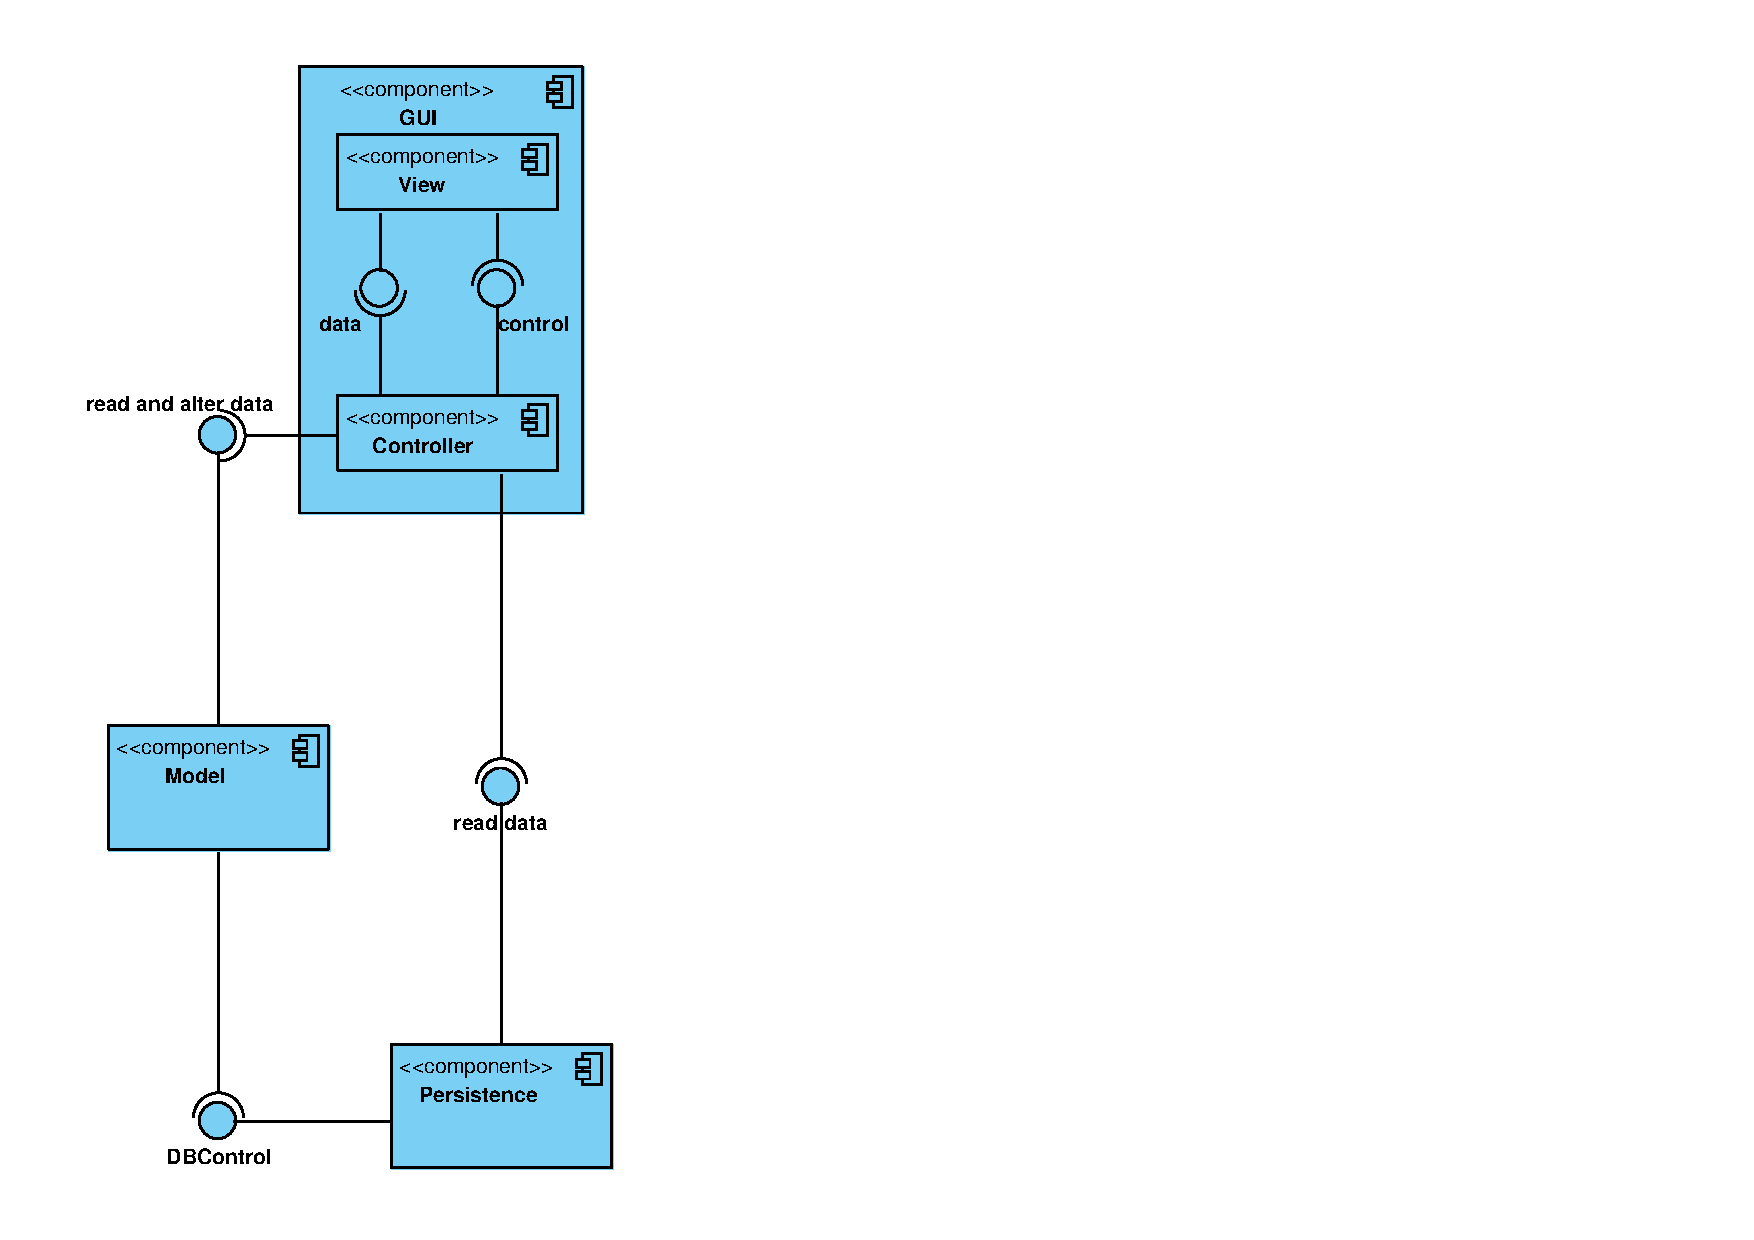
\includegraphics[width=0.45\textwidth]{konzeptsicht.pdf}
\end{figure}


Der Client besteht aus der GUI-, Model- und Persistence-Komponente. Die GUI-Komponente ist wiederum unterteilt in View und Controller. Die View-Komponente stellt Daten (in Form von Eingaben des Nutzers) für die Controller-Komponente bereit. Die Controller-Komponente kontrolliert die Darstellung der View-Komponente und nutzt durch die Model-Komponente bereitgestellte Möglichkeiten, Daten zu modifizieren oder bestimmte verarbeitete Daten zu erhalten. Auch nutzt die Controller-Komponente die von der Persistence-Komponente bereitgestellten Operationen um Daten aus der Datenbank zu lesen. Die Model-Komponente enthält die gesamte Geschäftslogik und die Datenobjekte. Sie nutzt durch die Persistence-Komponente bereitgestellte Operationen, greift jedoch nicht nur auf lesende Operationen, sondern auch auf schreibende Methoden zu. Die Persistence-Komponente ist unabhängig von den anderen Komponenten.\\

Die Software ist grundsätzlich nach der hier aufgeführten Schichtenarchitektur aufgebaut:

\begin{figure}[H]
\centering
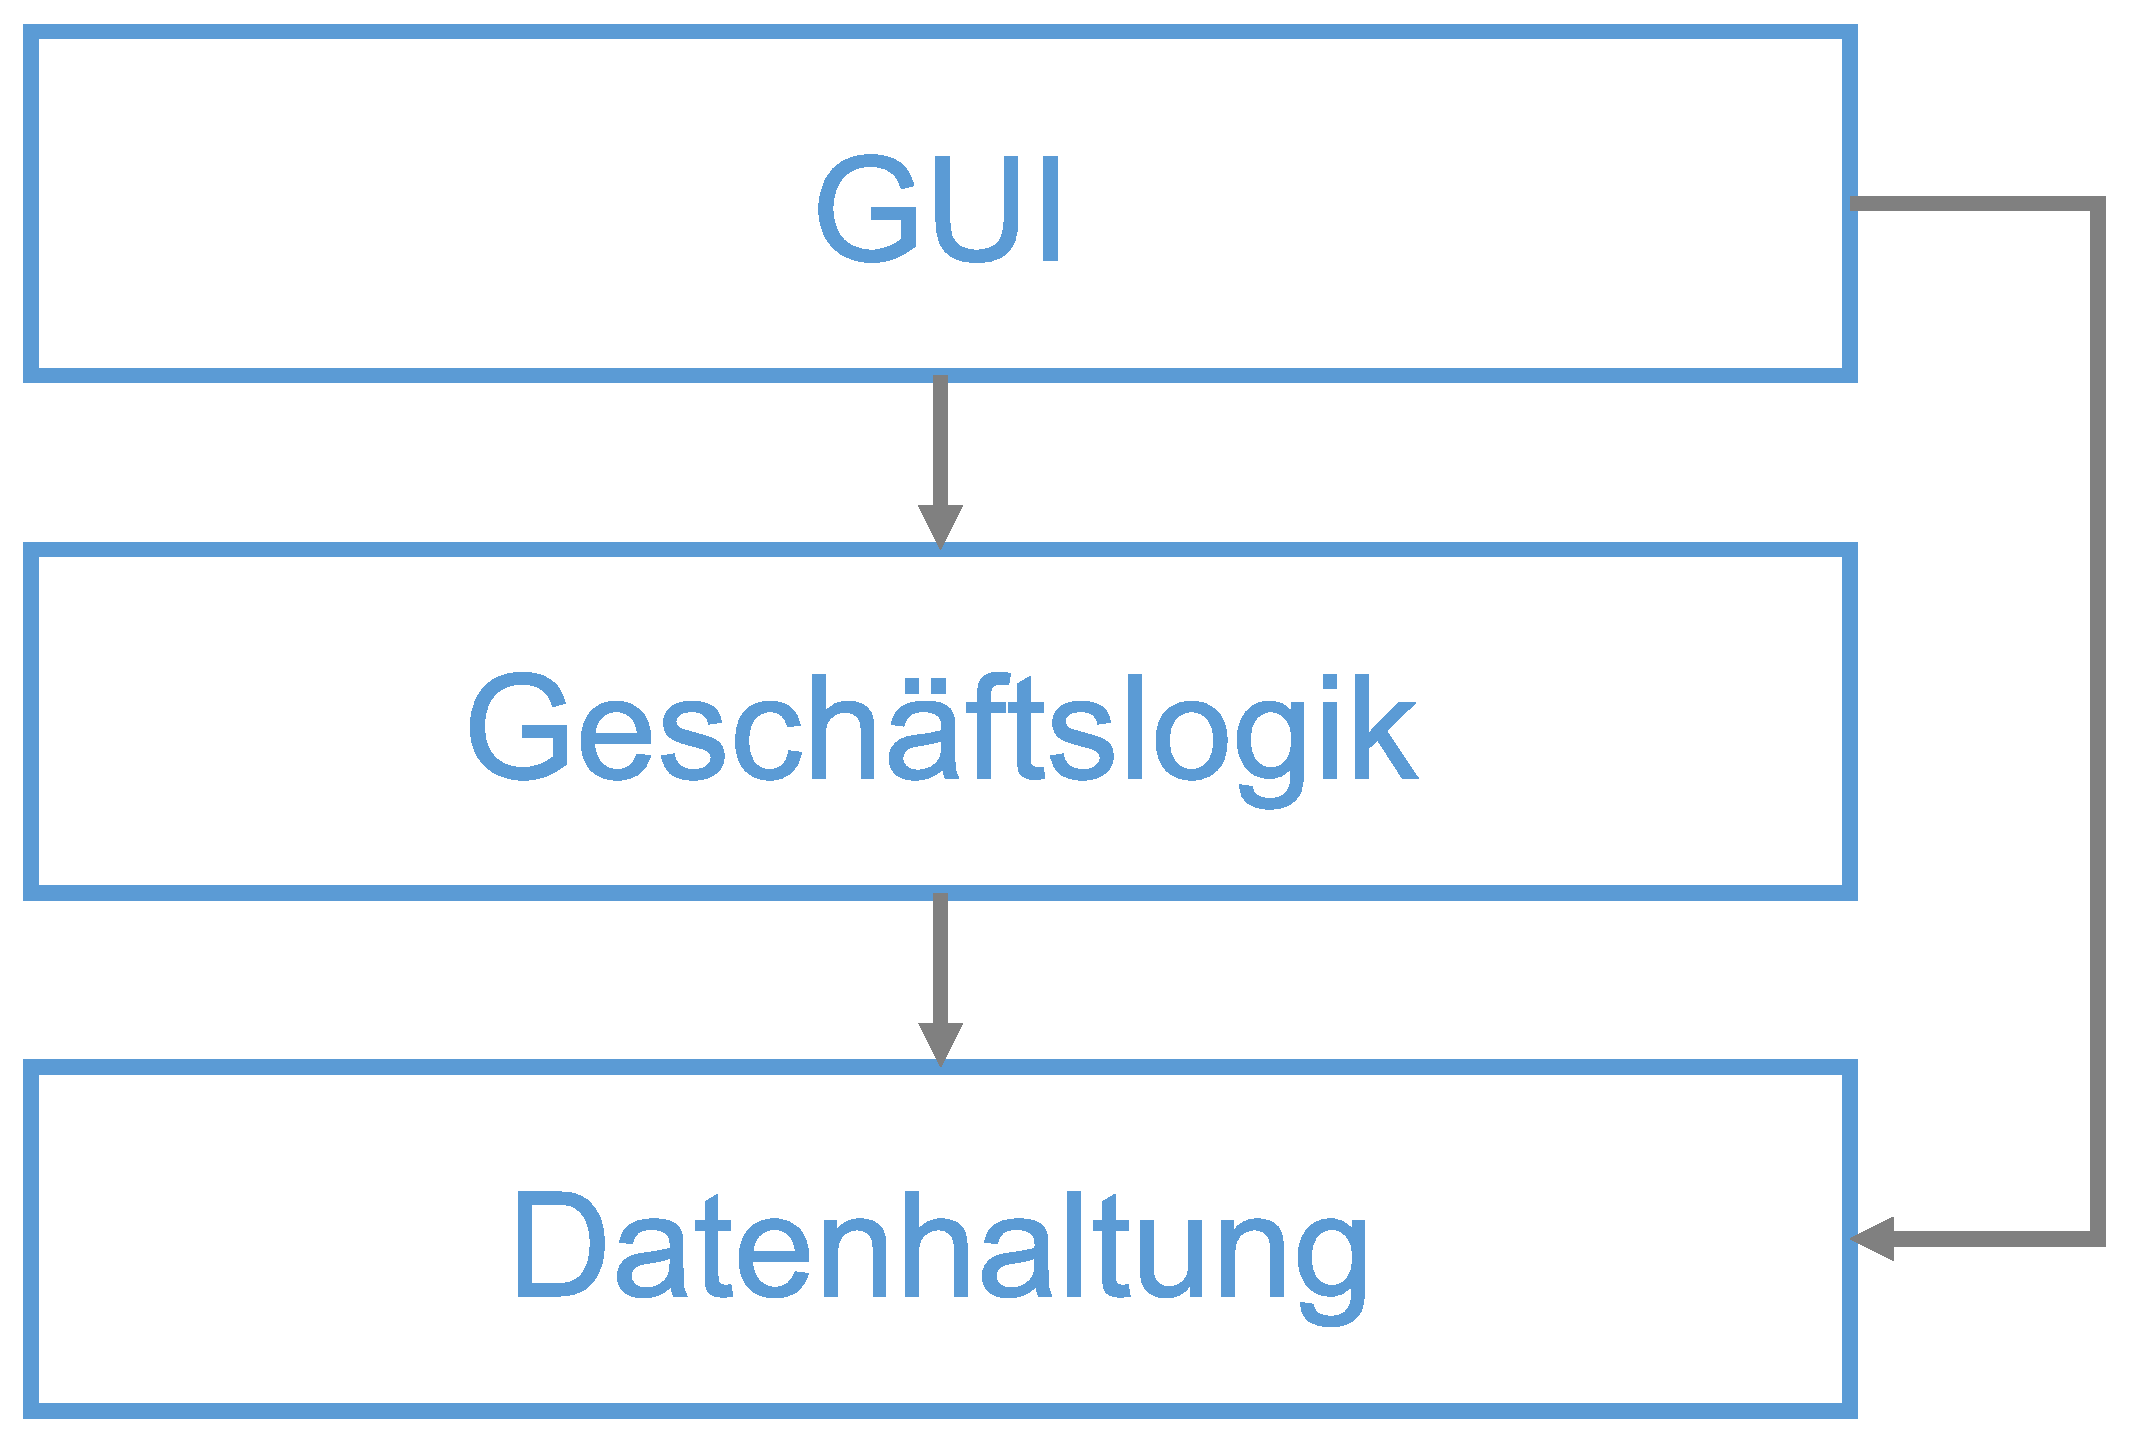
\includegraphics[width=0.5\textwidth]{schichten.pdf}
\end{figure}

Jede höhere Ebene greift nur auf niedriger liegende Ebenen zu. Die GUI-Schicht stellt die GUI-Komponente, die Geschäftslogik-Schicht die Model-Komponente und die Datenhaltung-Schicht die Persistence-Komponente dar. Die GUI-Schicht darf auch direkt auf die Datenhaltung-Schicht zugreifen, ruft jedoch nur lesende Methoden auf, während die Geschäftslogik-Schicht auch schreibende Methoden aufruft.


\section{Modulsicht}
\label{sec:modulsicht}

\subsection{Paketdiagramm}
Die Software ist aufgeteilt in fünf große Pakete, die jeweils noch Unterpakte besitzen. Die View-Komponente wurde im nachfolgenden Diagramm nur als Paket aufgeführt, um die Abhängigkeiten aufzeigen zu können. Dies entspricht nicht der tatsächlichen Organisationsstruktur. Um das Diagramm übersichtlicher zu halten, wurden fast ausschließlich die Abhängigkeiten zwischen den großen Pakten aufgeführt. Lediglich für das Paket \textit{org.woym.ui} wurde eine etwas detaillierte Darstellung gewählt.

\begin{figure}[H]
\centering
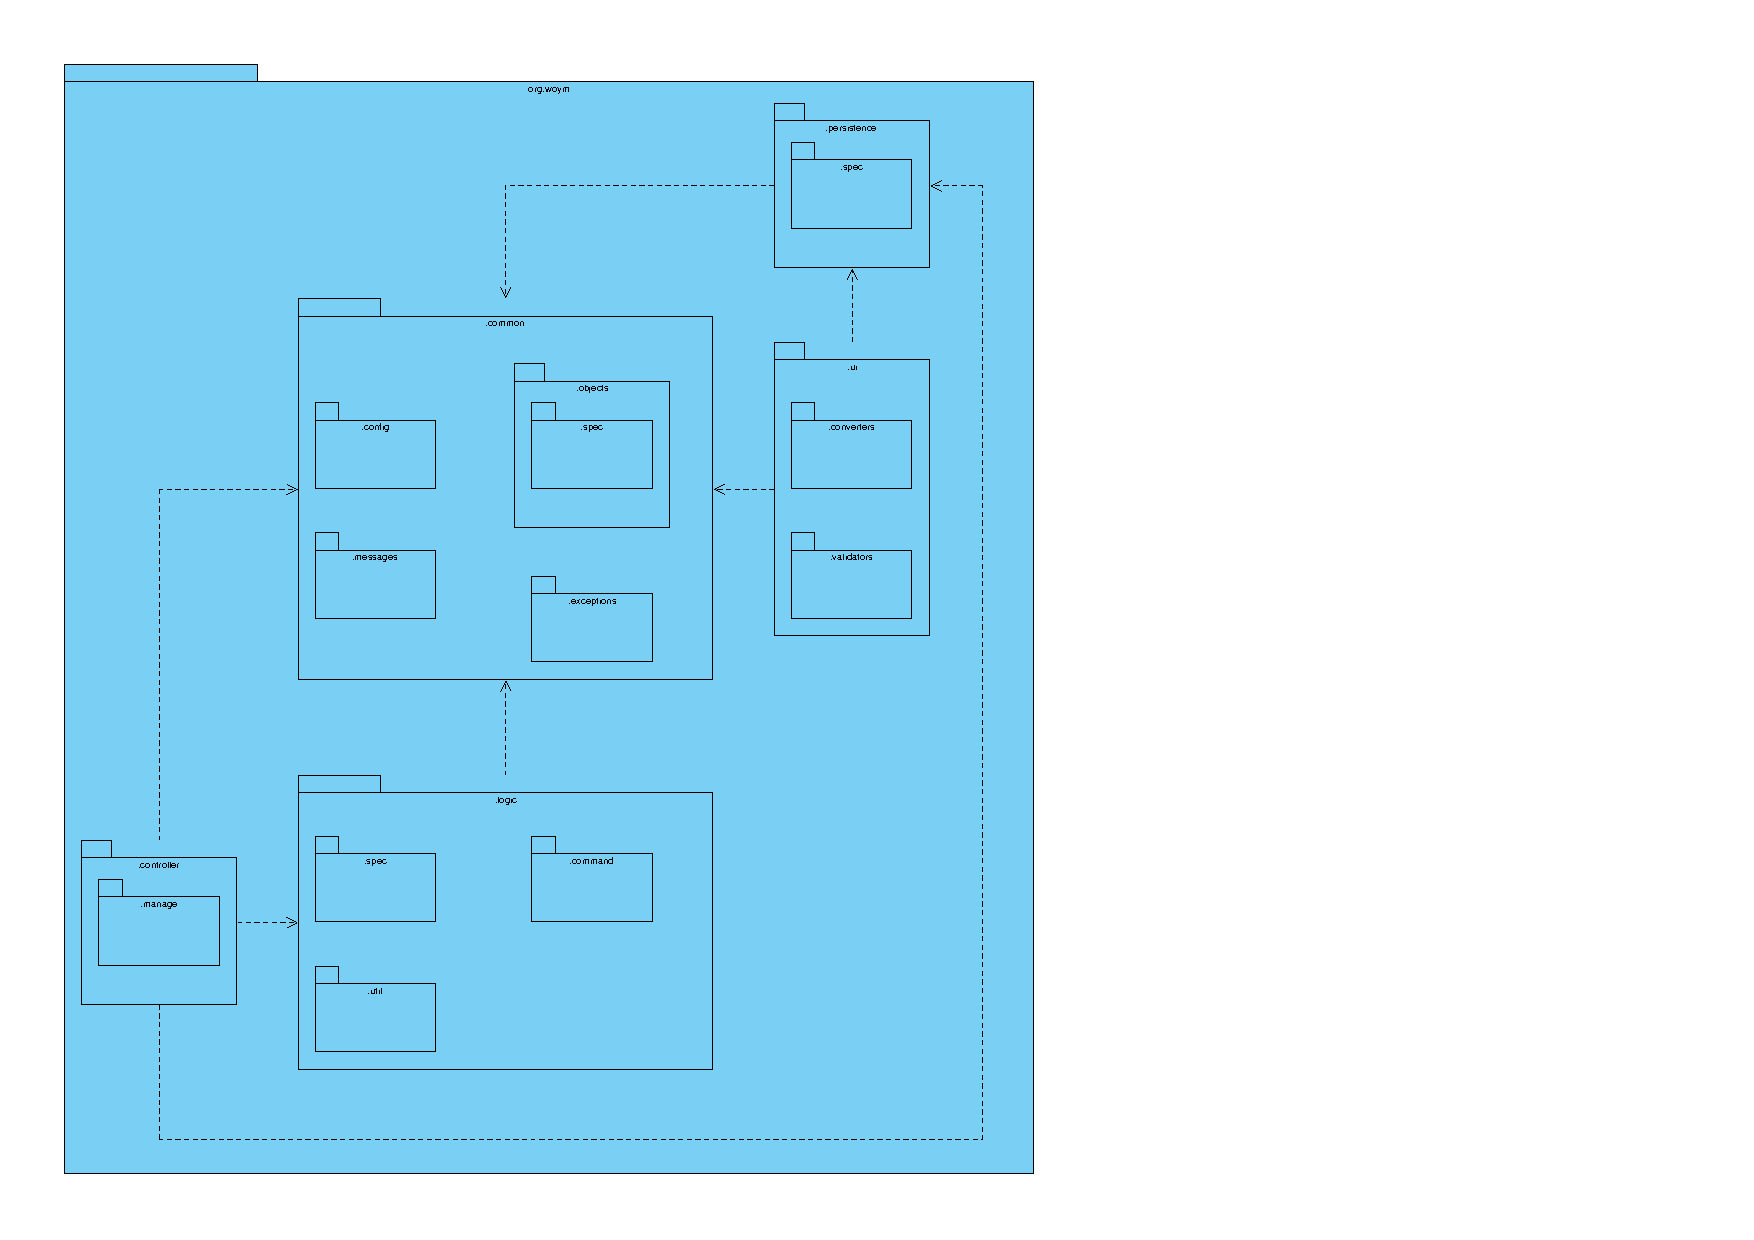
\includegraphics[width=\textwidth]{packages.pdf}
\end{figure}

\newpage

\begin{itemize}
\item \textit{org.woym.persistence}: In diesem Paket befinden sich alle Klassen, die Methoden für lesenden oder schreibenden Zugriff auf der Datenbank enthalten. Im Unterpaket \textit{org.woym.persistence.spec} befinden sich die zugehörigen Interfaces (s. Kapitel \ref{subsec:persistence}). Dieses Paket stellt die Persistence-Komponente aus der konzeptionellen Sicht dar.
\item \textit{org.woym.common}: In diesem Paket  bzw. in den jeweiligen Unterpaketen befinden sich Klassen, welche von Klassen aus fast allen anderen Paketen verwendet werden (s. Kapitel \ref{subsec:Common}). Eine konkrete Einordnung dieses Paketes in die konzeptionelle Sicht ist nicht möglich. 
\item \textit{org.woym.controller}: Dieses Paket enthält alle Controller, welche die Eingaben von der GUI verarbeiten (s. Kapitel \ref{subsec:Controller}, damit entspricht dieses Paket der Controller-Komponente aus der konzeptionellen Sicht.
\item \textit{org.woym.ui}: Dieses Paket enthält JSF-Validatoren und -Converter, sowie Hilfsklassen, welche Daten für die Controller so aufbereiten, dass Sie von der View-Komponente korrekt dargestellt werden können. (s. Kapitel \ref{subsec:UI}). Dieses Paket befindet sich grundsätzlich in der Geschäftslogik-Schicht. Die Validatoren und Converter sind jedoch nicht der Model-Komponente zuordenbar, da sie der View-Komponente direkt bekannt sind. 
\item \textit{org.woym.logic}: In diesem Paket befinden sich alle Klassen, die die Geschäftslogik implementieren (s. Kapitel \ref{subsec:logic}). Dieses Pakte stellt die Model-Komponente aus der konzeptionellen Sicht dar.
\end{itemize}

\subsection{Persistence}
\label{subsec:persistence}

Die Persistenzschicht ist für ein Single-User-System konzipiert und besteht aus drei Klassen. Die Singleton-Klasse \texttt{DataBase} stellt die unterste Ebene dar. Dort wird der EntityManager erzeugt, der für alle Datenbankanfragen von \texttt{DataAccess} verwendet wird. Außerdem bietet sie Methoden an, die ein Backup der Datenbank erzeugen bzw. ein Backup wiederherstellen. \texttt{DataBase} erweitert die Java-Klasse \texttt{Observable}, da es für die Wiederherstellung eines Backups notwendig ist, die Datenbank einmal komplett herunterzufahren und danach dementsprechend ein neuer EntityManager verwendet wird. Dies muss den beobachtenden Klassen mitgeteilt werden.\\
Die Singleton-Klasse \texttt{DataAccess} implementiert das Java-Interface \texttt{Observer} und wird bei Erzeugung bei \texttt{DataBase} als Observer registriert. Zudem implementiert sie das Interface \texttt{IDataAccess}, welches alle DAO-Interfaces implementiert und damit die notwendigen Datenzugriffsmethoden beschreibt. Die Klasse \texttt{DataAccess} stellt also für alle Klassen auf einer oberen Ebene die Schnittstelle zur Datenbank dar.\\
Die letzte Klasse der Persistenzschicht ist \texttt{DataBaseServletListener}, welche das Java-Interface \texttt{ServletContextListener} implementiert. Sie ruft mit dem Start des Servlet-Containers die \textit{setUp()}-Methode von \texttt{DataBase} auf.\\

Bevor die Methoden von \texttt{DataAcess} oder \texttt{DataBase} verwendet werden können, muss mindestens einmal die Methode \textit{setUp()} der Klasse \texttt{DataBase} aufgerufen werden, da diese den von \texttt{DataAccess} benötigten EntityManager erzeugt.\\
Die Methoden des Interfaces \texttt{IDataAccess} dürfen in beliebiger Reihenfolge aufgerufen werden. Methoden, welche als Rückgabewert eine Liste haben, geben in allen Fällen eine Liste zurück, diese kann also leer sein. Methoden, welche als Rückgabewert ein einzelnes Objekt einer Klasse besitzen, geben ein gemäß der JavaDoc-Beschreibung entsprechendes Objekt der Klasse oder \textbf{null} zurück, falls kein entsprechendes Objekt vorhanden ist. 


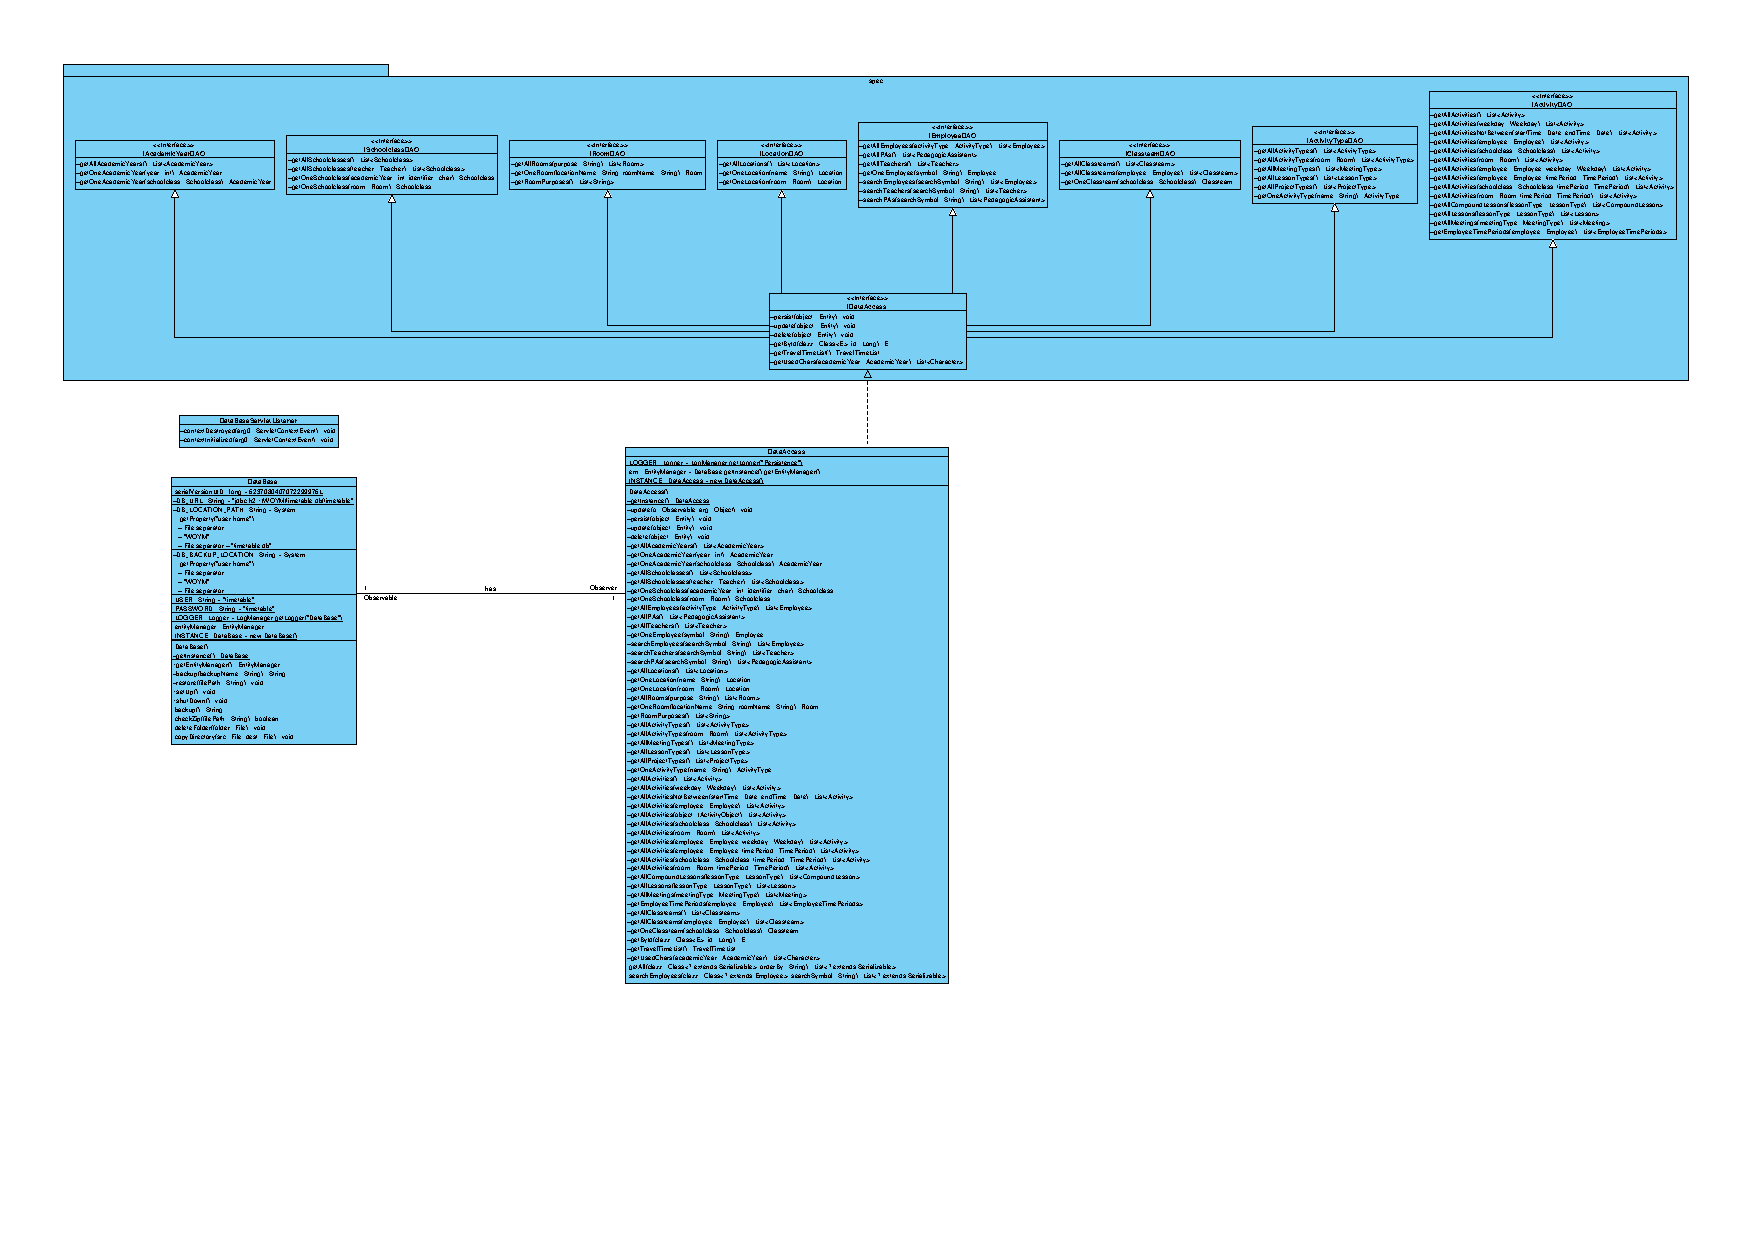
\includepdf[landscape]{persistence.pdf}


\subsection{Common}
\label{subsec:Common}
Im Paket \textit{org.woym.common} befinden sich -- wie vorher bereits angemerkt -- Klassen, welche von Klassen aus fast allen anderen Paketen verwendet werden.\\
Das Paket \textit{org.woym.common.config} beinhaltet das \texttt{DefaultConfigEnum}, welches alle Einstellungsoptionen der Software mit ihren Standardwerten enthält. Die Klasse \texttt{Config} erzeugt eine Properties-Datei und gewährt anderen Klassen Zugriff auf dort eingetragene Werte. Bevor die anderen Methoden der Klasse aufgerufen werden können, muss mindestens einmal die Methode \textit{init()} aufgerufen werden. 
\\
Die Klasse \texttt{ConfigServletListener} implementiert das Java-Interface \texttt{ServletContextListener} und sorgt dafür, dass mit dem Start des Servlet-Containers einmal die \textit{init()}-Methode von \texttt{Config} aufgerufen wird.\\

Das Paket \textit{org.woym.common.messages} beinhaltet vier Enums mit Statusnachrichten. Die Klasse \texttt{MessageHelper} stellt Methoden bereit, welche für die Übergabe einer entsprechenden Nachricht und ggf. zusätzlichen Parametern eine \texttt{FaceMessage} zurückgibt. Die Methoden können in beliebiger Reihenfolge aufgerufen werden.\\

Das Paket \textit{org.woym.common.exceptions} enthält lediglich die selbst angelegten Exceptions. \\

Das Paket \textit{org.woym.common.objects} ist hier nicht vollständig dargestellt (s. Kapitel \ref{subsubsec:Objects}), da dies zu unübersichtlich wäre, stattdessen ist nur das Unterpaket \textit{org.woym.common.objects.spec} dargestellt. Dieses enthält drei Interfaces. \texttt{IMemento} dient lediglich der Vereinheitlichung aller einzelnen Memento-Klassen unter einem gemeinsamen Interface. Da die Memento-Klassen nach außen hin vollständig opak sind und keinerlei Methoden bereitstellen, ist es sinnvoll, sie unter einem Interface zu vereinheitlichen, um sie von außen als gleichrangige Klassen zu verwenden. Das Interface \texttt{IActivityObject} dient der Vereinheitlichung von Klassen, deren Objekte Teil der Klasse \texttt{Activity} sein können. \\
Das Interface \texttt{IMementoObject} stellt Methoden für alle Klassen bereit, welche eine eigene Memento-Klasse definieren.\clearpage


\begin{figure}[H]
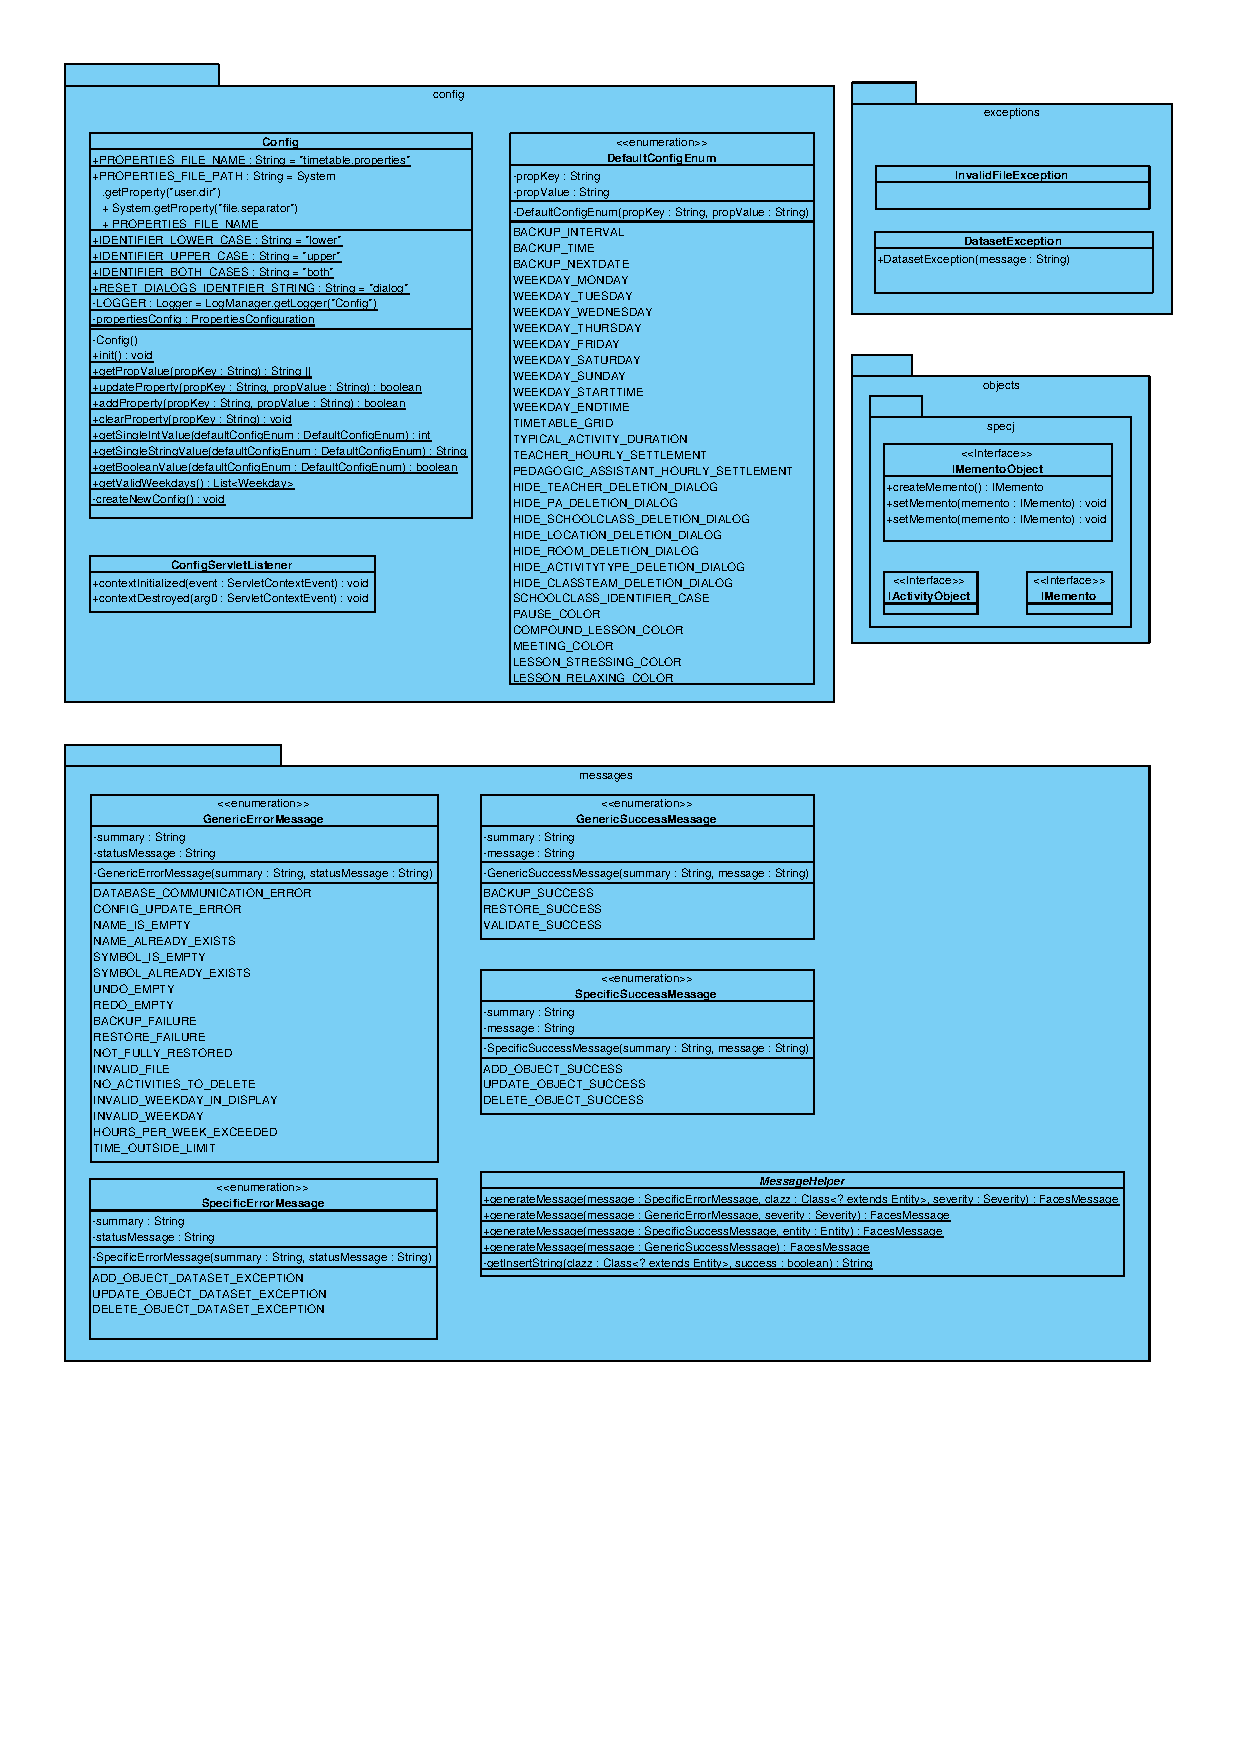
\includegraphics[width=\textwidth]{common.pdf}
\end{figure}
\newpage

\subsubsection{Objects}
\label{subsubsec:Objects}
Das auf der folgenden Seite dargestellte Klassendiagramm stellt das Paket \textit{org.woym.common.objects} dar. Es enthält im Gegensatz zu dem in Kapitel \ref{sec:datensicht} dargestellten Diagramm noch eine implementierungsspezifische Details, die nachfolgend erläutert werden sollen. Eine größere und übersichtlichere Darstellung des Diagramms war aufgrund der großen Anzahl an Kanten nicht möglich.\\
Ein Detail, welches hervorgehoben werden sollte, ist, dass alle Entitäten die gemeinsame abstrakte Superklasse \texttt{Entity} (linke Seite, mittlere Höhe) besitzen. Die Vereinheitlichung unter dieser Klasse wird an einigen Stellen genutzt, um eine etwas allgemeinere Implementierung zu ermöglichen. Zudem stellt sie eine \textit{persist}-, \textit{update}-, \textit{delete} und \textit{refresh}-Methode für die erbenden Klassen bereit.\\
Ansonsten sollte auch die Teil-von-Beziehung zwischen den Entitäten und den zugehörigen Memento-Klassen herauszustellen. Die Memento-Klassen sind statische innere Klassen ihrer jeweiligen Entitätenklasse und bieten einen package-private Konstruktor, so dass dieser ansonsten nicht von außen verwendet werden kann. Auch bieten die Mementos nach außen hin keine Methoden. Sie sind also für alle anderen Klassen -- außer der zugehörigen Entitätenklasse -- vollständig opak.\\
Für die Speicherung von Wegzeiten existiert die Singleton-Klasse \texttt{TravelTimeList} (oben links), welche die statische Klasse \texttt{Edge} enthält. Eine Liste von \texttt{Edge}-Objekten in \texttt{TravelTimeList} repräsentiert die Wegzeiten zwischen je zwei Standorten. Es existiert immer nur ein \texttt{TravelTimeList}-Objekt in der Datenbank. Ist bei Aufruf von \textit{getInstance} noch keines vorhanden, wird eins angelegt.\\
Ein übersichtlicheres Datenmodell befindet sich in Kapitel \ref{sec:datensicht}. Dort werden auch alle weiteren Relevanten Assoziationen erläutert.

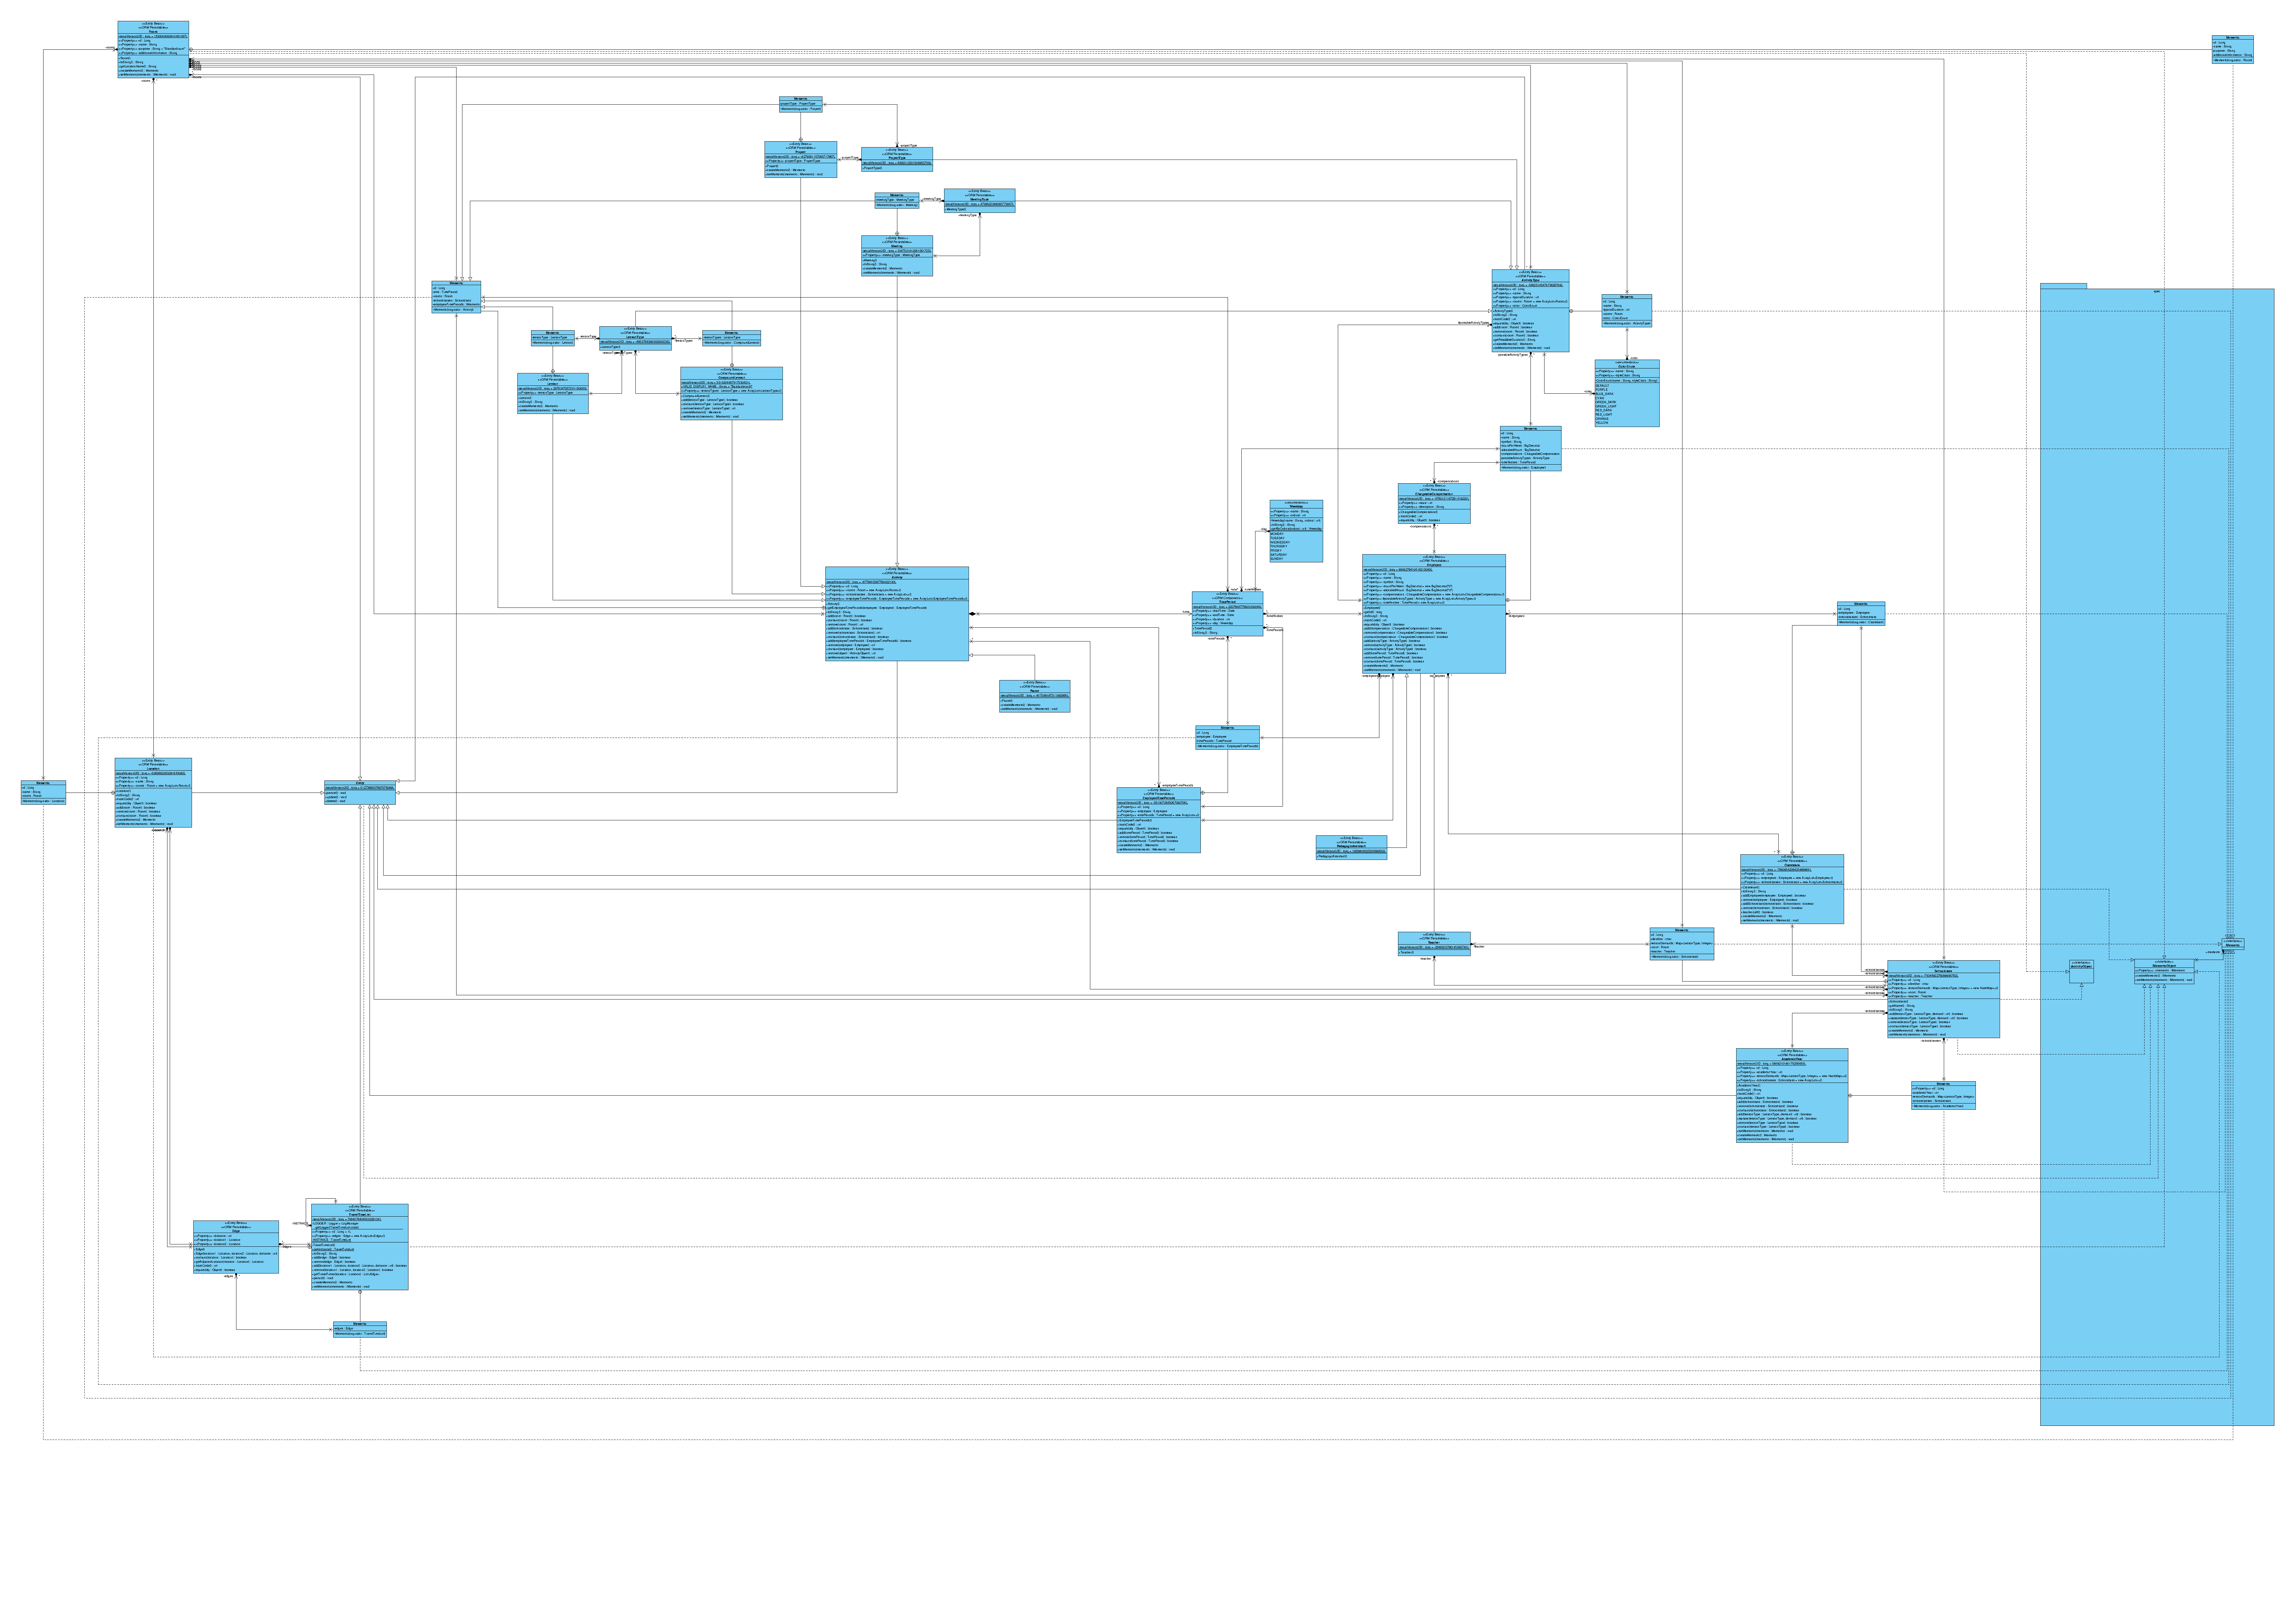
\includepdf[landscape]{objects.pdf}


\subsection{Controller}
\label{subsec:Controller}

Im Paket \textit{org.woym.controller} befinden sich die Backing Beans für die verschiedenen JSF-Seiten. \\
Die Klasse \texttt{GUIController} stellt den Aufruf der Undo- und Redo-Funktionalität aus dem \texttt{CommandHandler} (s. Kapitel \ref{subsec:logic}) für alle JSF-Seiten bereit und befindet sich daher im übergeordneten Paket.\\
Im Paket \textit{org.woym.controller.manage} befinden sich die Backing Beans für die JSF-Seiten der Systemeinrichtung und im Paket \textit{org.woym.controller.planning} die Backing Beans für die JSF-Seiten der Planung. In der Systemeinrichtung besitzt jede JSF-Seite einen eigenen Controller. Auf der Planungsseite ist der \texttt{PlanningController} für die Darstellung und Funktionalität der Seite vorhanden. Lediglich die Operationen für die Dialoge zum Hinzufüge von Aktivitäten wurden in einzelne Controller ausgelagert.\\
Der Zusammenhang zwischen den JSF-Seiten und den Controllern ist hier nicht darstellbar.

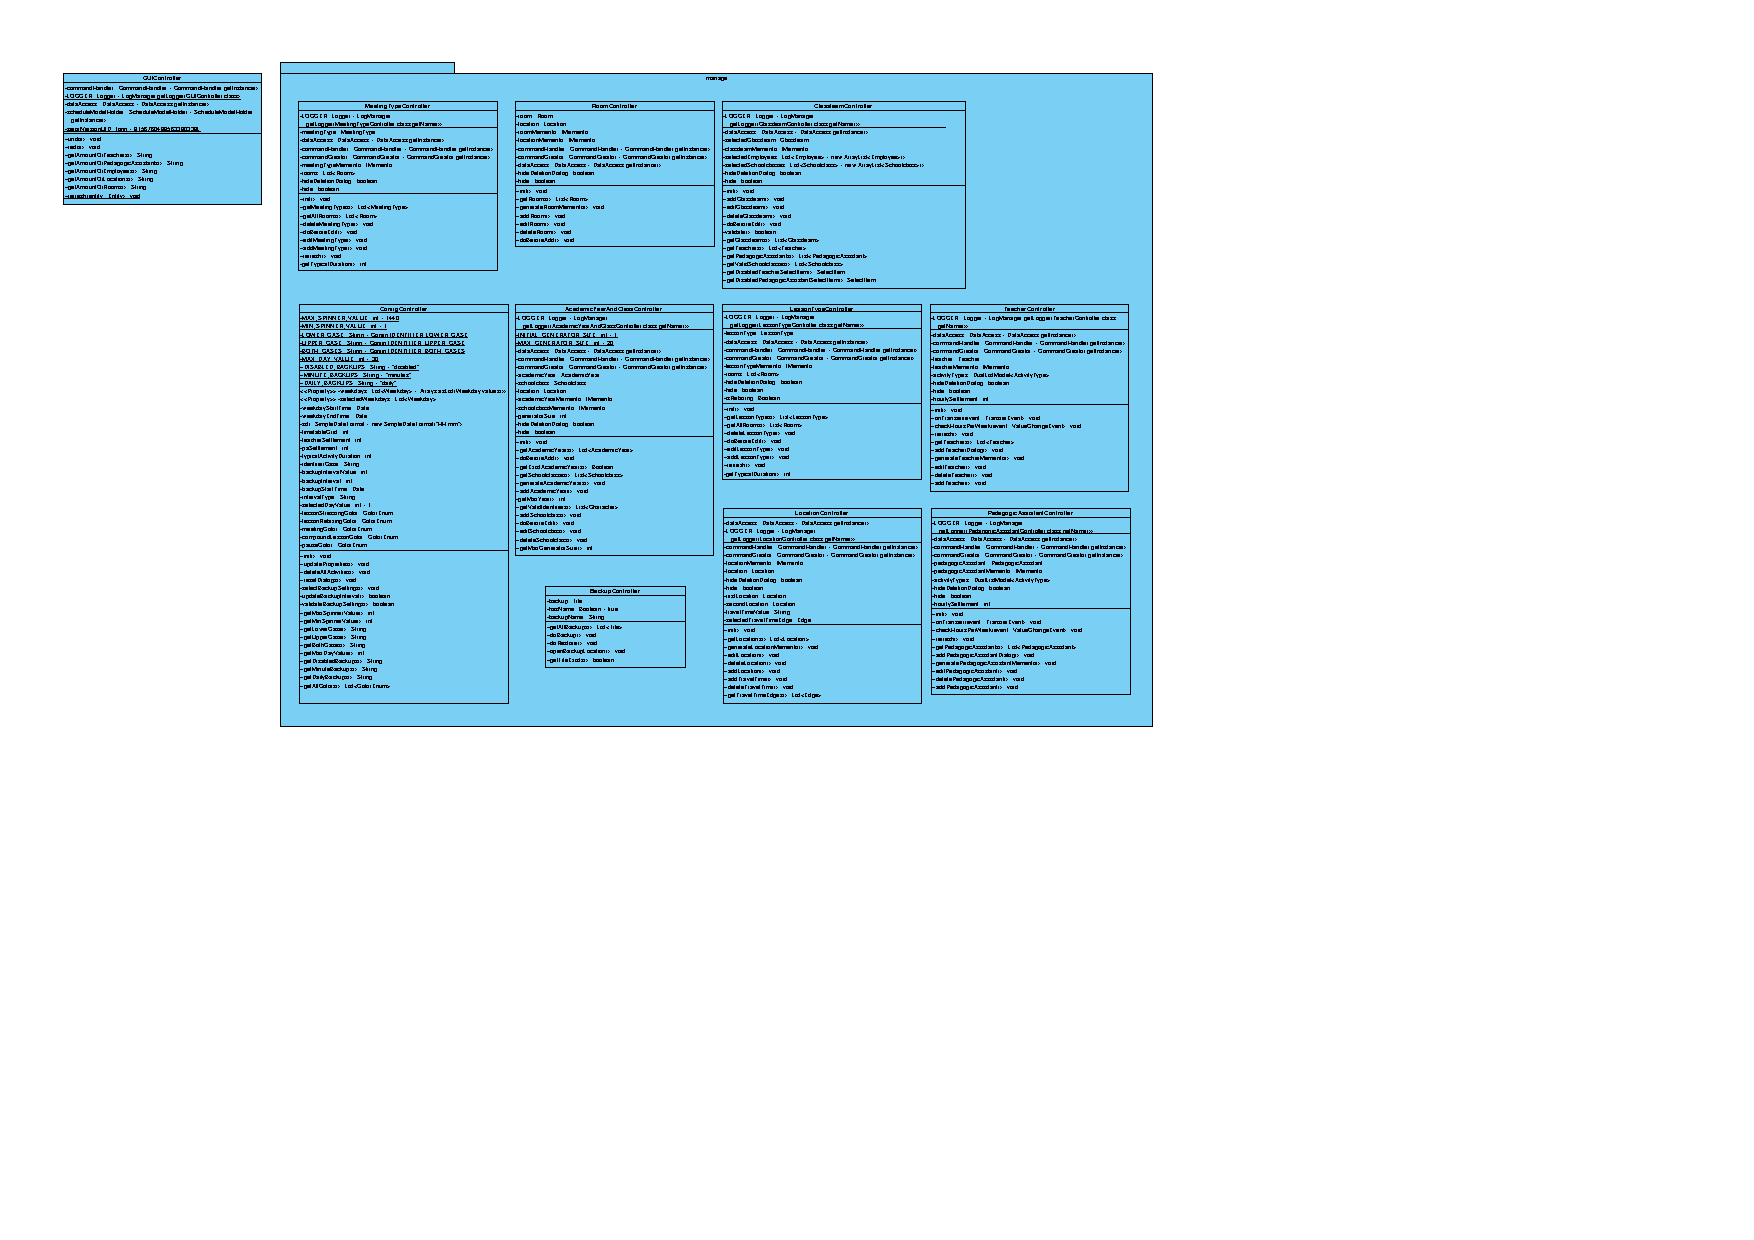
\includepdf[landscape]{controller.pdf}

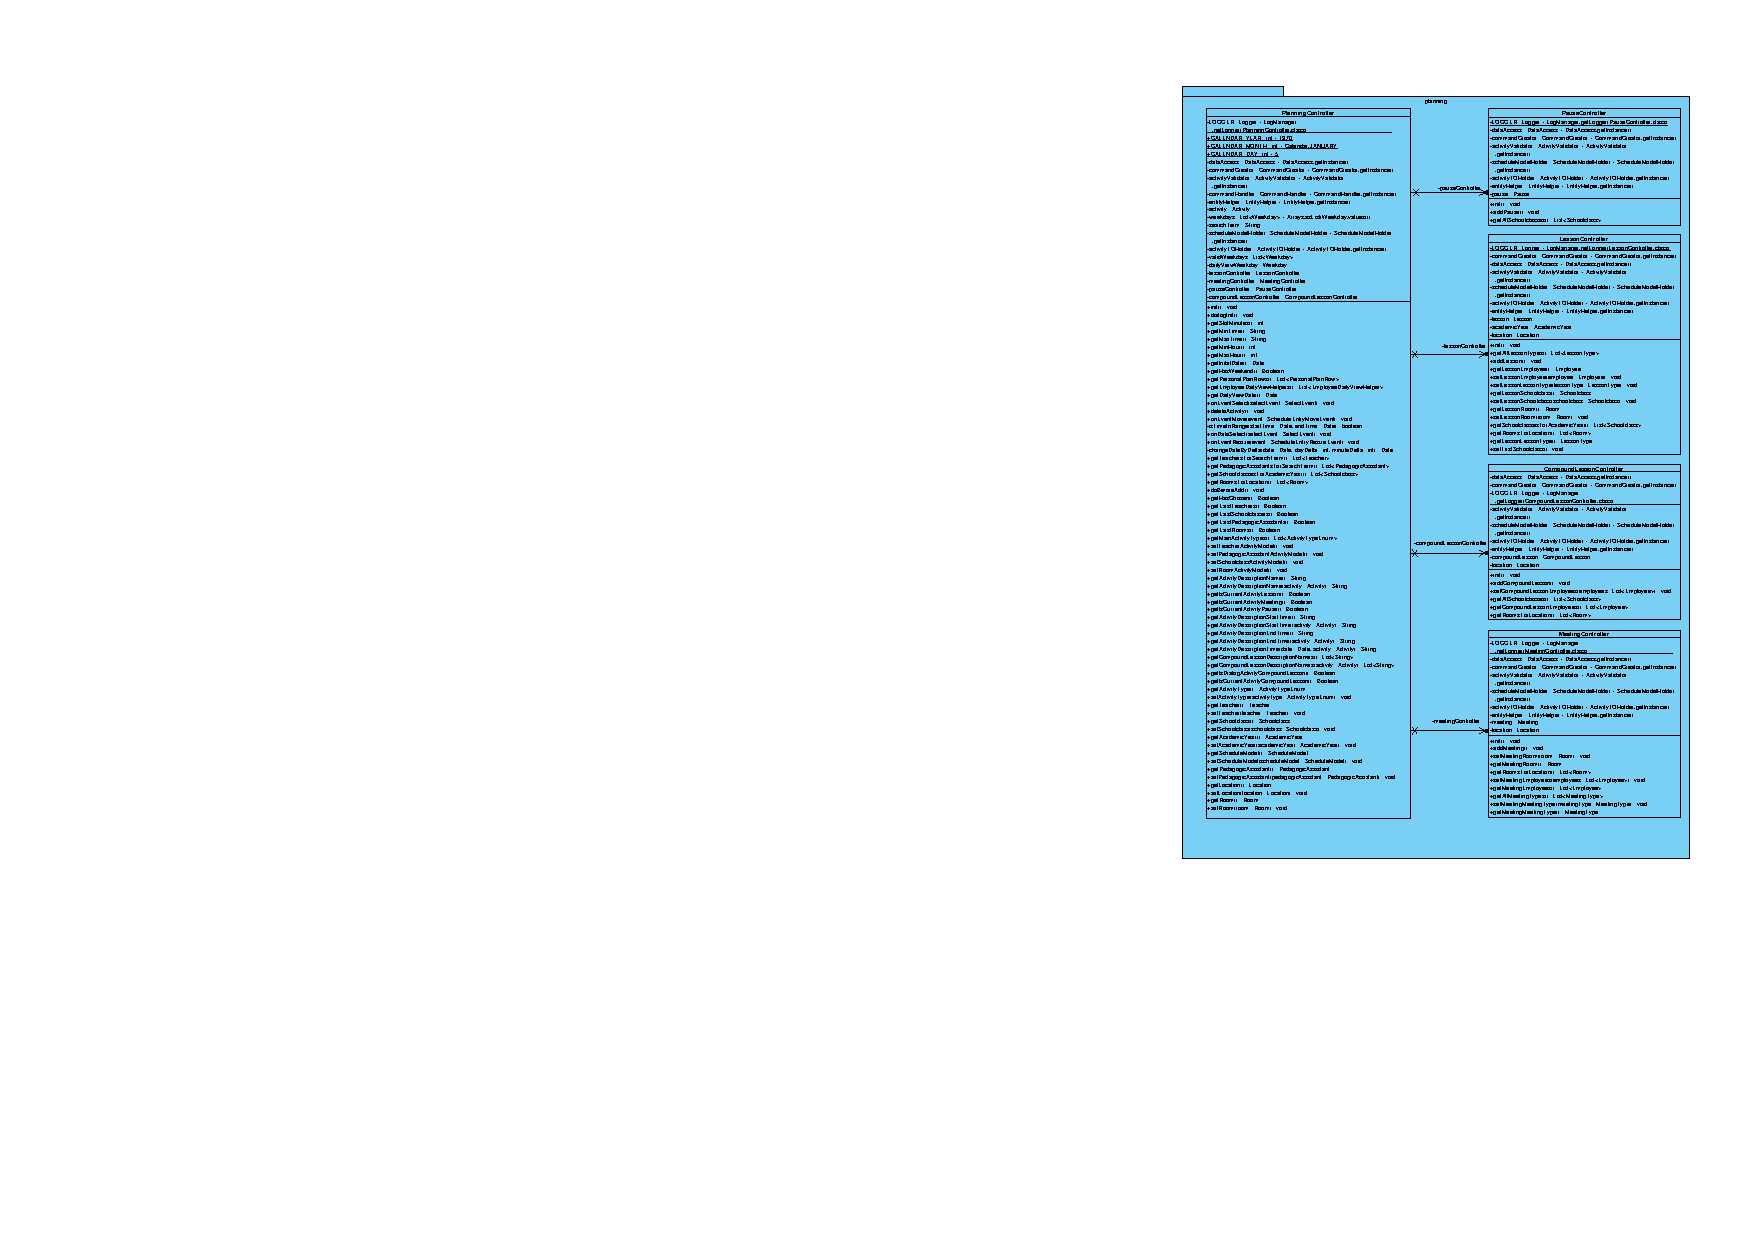
\includepdf{controller2.pdf}

\subsection{UI}
\label{subsec:UI}

Im Paket \textit{org.woym.ui.converters} befinden sich die JSF-Converter und im Paket \textit{org.woym.ui.validators} die JSF-Validatoren. Das Paket \textit{org.woym.ui.util} enthält Hilfsklassen für die Backing Beans der Planungsseite. Diese Hilfsklassen dienen im Wesentlichen der Unterstützung zur korrekten Darstellung der Elemente auf dieser Seite.\clearpage

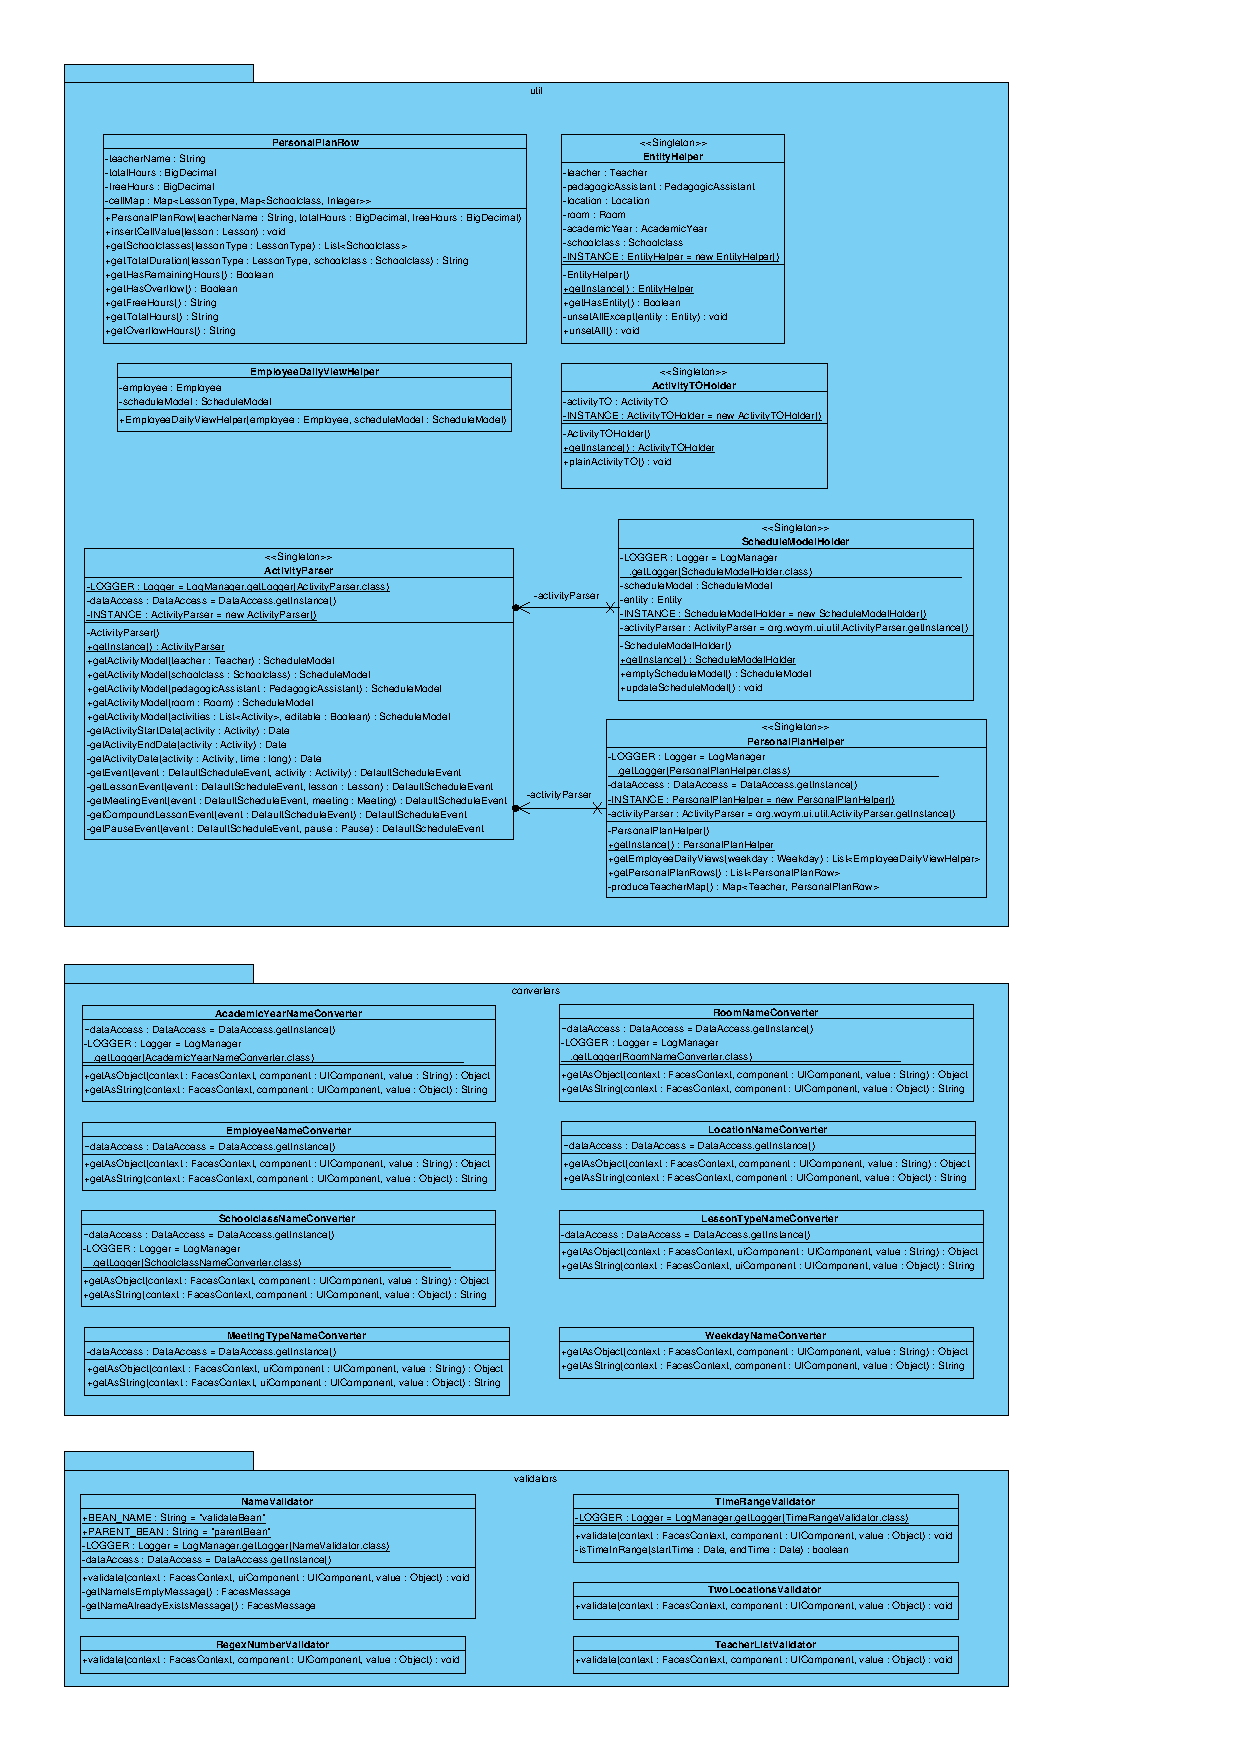
\includepdf{ui.pdf}


\subsection{Logic}
\label{subsec:logic}
Auf der Logikebene wurde das Command-Pattern verwendet, um ein Undo und Redo für alle Aktionen anbieten zu können. Die entsprechenden Klassen befinden sich im Paket \textit{org.woym.logic.command}. \\
Das Interface \texttt{ICommand} spezifiziert die Methoden eines konkreten Commands. Implementiert wird das Interface von den Klassen \texttt{AddCommand}, \texttt{UpdateCommand}, \texttt{DeleteCommand} und \texttt{MacroCommand}. Wobei ein \texttt{MacroCommand} zusätzlich eine Liste von \texttt{ICommand}-Objekten enthält. Für die Methoden gibt es eine klare Ausführungsreihenfolge. Nach Erzeugung eines ICommand-Objektes muss zunächst \textit{execute()} aufgerufen werden, danach dürfen alternierend \textit{undo()} und \textit{redo()} beliebig oft aufgerufen werden. \\

Neben den Commands befindet sich im Paket \textit{org.woym.logic.command} auch die Singleton-Klasse \texttt{CommandCreator}, welche nach dem Factory-Entwurfsmuster drei öffentliche Methode \textit{createDeleteCommand(Entity)}, \textit{createEmployeeUpdateAddWorkingHours(Activity)} und \textit{createEmployeeUpdateSubtractWorkingHours(Activity)} anbietet. Die Methode \textit{createDeleteCommand(Entity)} erzeugt für ein übergebenes \textit{Entity}-Objekt ein MacroCommand zum Löschen dieses Objektes, welches in der korrekten Abfolge alle Abhängigkeiten auflöst, und gibt dieses zurück. Die Methode darf beliebig aufgerufen werden. Für nähere Informationen siehe JavaDoc.\\
Die anderen beiden Methoden erzeugen jeweils ein \texttt{MacroCommand}, welches allen Mitarbeitern der übergebenen Aktivität entweder die Dauer ihrer Teilnahme an der Aktivität zu den verteilten Wochenstunden dazu addiert oder sie abzieht, und geben dieses zurück.\\

Im Paket \textit{org.woym.logic} befindet sich dann die Klasse \texttt{CommandHandler}, diese übernimmt für die korrekte Undo-/Redo-Funktionalität die Ausführung der Commands. Für die Ausführungsreihenfolge der Methoden gilt dasselbe, wie für die \texttt{ICommand}-Implementierungen. Der \texttt{CommandHandler} besitzt zwei Listen vom Typ \texttt{ILimitedQueue}. Die eine speichert alle Commands, die rückgängig gemacht werden sollen, die andere alle Commands, die wiederholt werden sollen. Bei einem Aufruf von \textit{execute(ICommand)} wird das Command also zunächst der Undo-Liste hinzugefügt, wird dann \textit{undo} aufgerufen, wird es der Redo-Liste hinzugefügt und bei anschließendem Aufruf von \textit{redo} wieder der Undo-Liste.\\
Im Paket \textit{org.woym.logic} befinden sich außerdem die zwei Implementierungen \texttt{SuccessStatus} und \texttt{FailureStatus} des Interfaces \textit{IStatus}. Diese repräsentieren die erfolgreiche bzw. fehlgeschlagene Ausführung einer Aktion.\\
Zudem befindet sich in dem Paket auch die Klasse \texttt{BackupRestoreHandler}. Diese implementiert das Interface \texttt{ServletContextListener}, so dass mit dem Start des Servlet-Containers der \texttt{ScheduledExecutorService} gestartet wird, welcher die automatischen Backups des Systems übernimmt. Für die Erstellung der Backups wird die Methode \textit{backup(String)} der Klasse verwendet. Diese führt ein Datenbankbackup durch Ausführung der Methode \textit{backup(String)} der Klasse \texttt{DataBase} aus und fügt diesem zusätzlich die Properties-Datei mit den aktuellen Systemeinstellungen hinzu. Die Methode \textit{restore(String)} stellt ein Datenbank-Backup unter Verwendung der Methode \textit{restore(String)} der Klasse \texttt{DataBase} wieder her. Zusätzlich wird die in dem Backup gespeicherte Properties-Datei wiederhergestellt. \\
Das Paket \textit{org.woym.logic.util} enthält -- abgesehen von der Klasse \texttt{LimitedQueue} -- Klassen, welche Logikoperationen unter Verwendung anderer Klasse aus dem Paket \textit{org.woym.logic} für Klassen des Paktes \textit{org.woym.controller} und dessen Subpakete bereitstellen. Die Klasse \texttt{SchoolclassIdentifierUtil} bietet eine Methode, welche alle gemäß den Einstellungen noch verfügbaren Bezeichner für Schulklassen des übergebenen Jahrgangs zurückgibt. In die Klasse \texttt{ConfigControllerUtil} wurden einige umfangreichere Operationen ausgelagert, die vom \texttt{ConfigController} benötigt werden. Die Methoden können grundsätzlich in beliebiger Reihenfolge aufgerufen werden.\\
Die Klasse \texttt{ActivityValidator} bietet fünf öffentliche Methoden, wobei lediglich die Methode \textit{validateActivity(Activity, TimePeriod)} vom \texttt{PlanningController} aufgerufen wird. Da diese Methode prüft, ob die übergebene Aktivität am übergebenen Zeitraum eingefügt werden kann oder ob eine Überschneidung vorliegt, wird sie vor dem finalen Hinzufügen oder Aktualisieren einer Aktivität aufgerufen.\\
Die Klasse \texttt{ActivityParser} überführt in den Methoden \textit{getActivityModel(Teacher)}, \textit{getActivityModel(Schoolclass)}, \textit{getActivityModel(PedagogicAssistant)} und \textit{getActivityModel(Room)} alle Aktivitäten des übergebenen Objektes in ein \texttt{ScheduleModel}, so dass diese optisch dargestellt werden können. Diese Methoden können in beliebiger Reihenfolge ausgeführt werden.
 
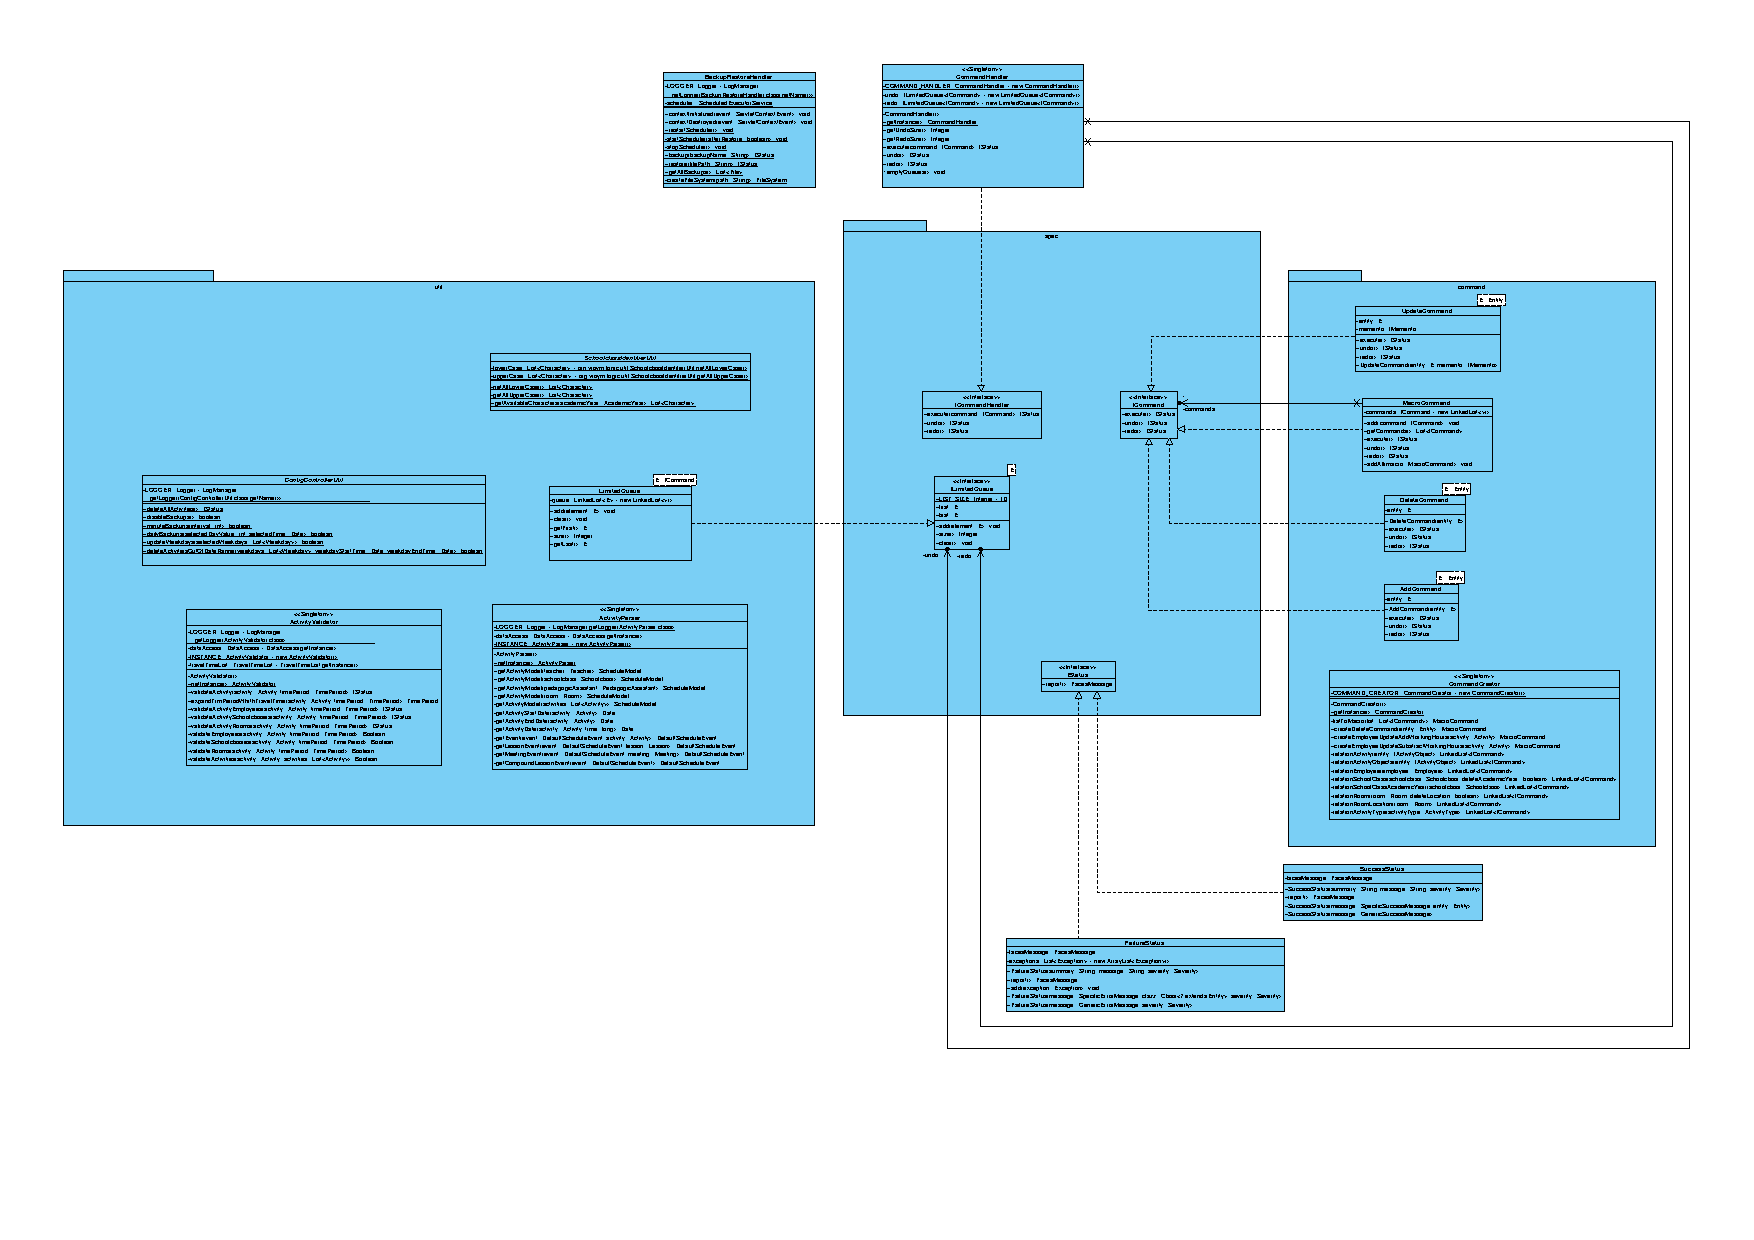
\includepdf{logic.pdf}





\section{Datensicht}
\label{sec:datensicht}
  
\subsection{Datenmodell}
Auf der folgenden Seite ist das Datenmodell dargestellt. Danach folgt eine Beschreibung der einzelnen Assoziationen. Das Datenmodel beinhaltet keine implementierungsspezifischen Details. Diese sind im Klassendiagramm zu Kapitel \ref{subsubsec:Objects} zu erkennen.
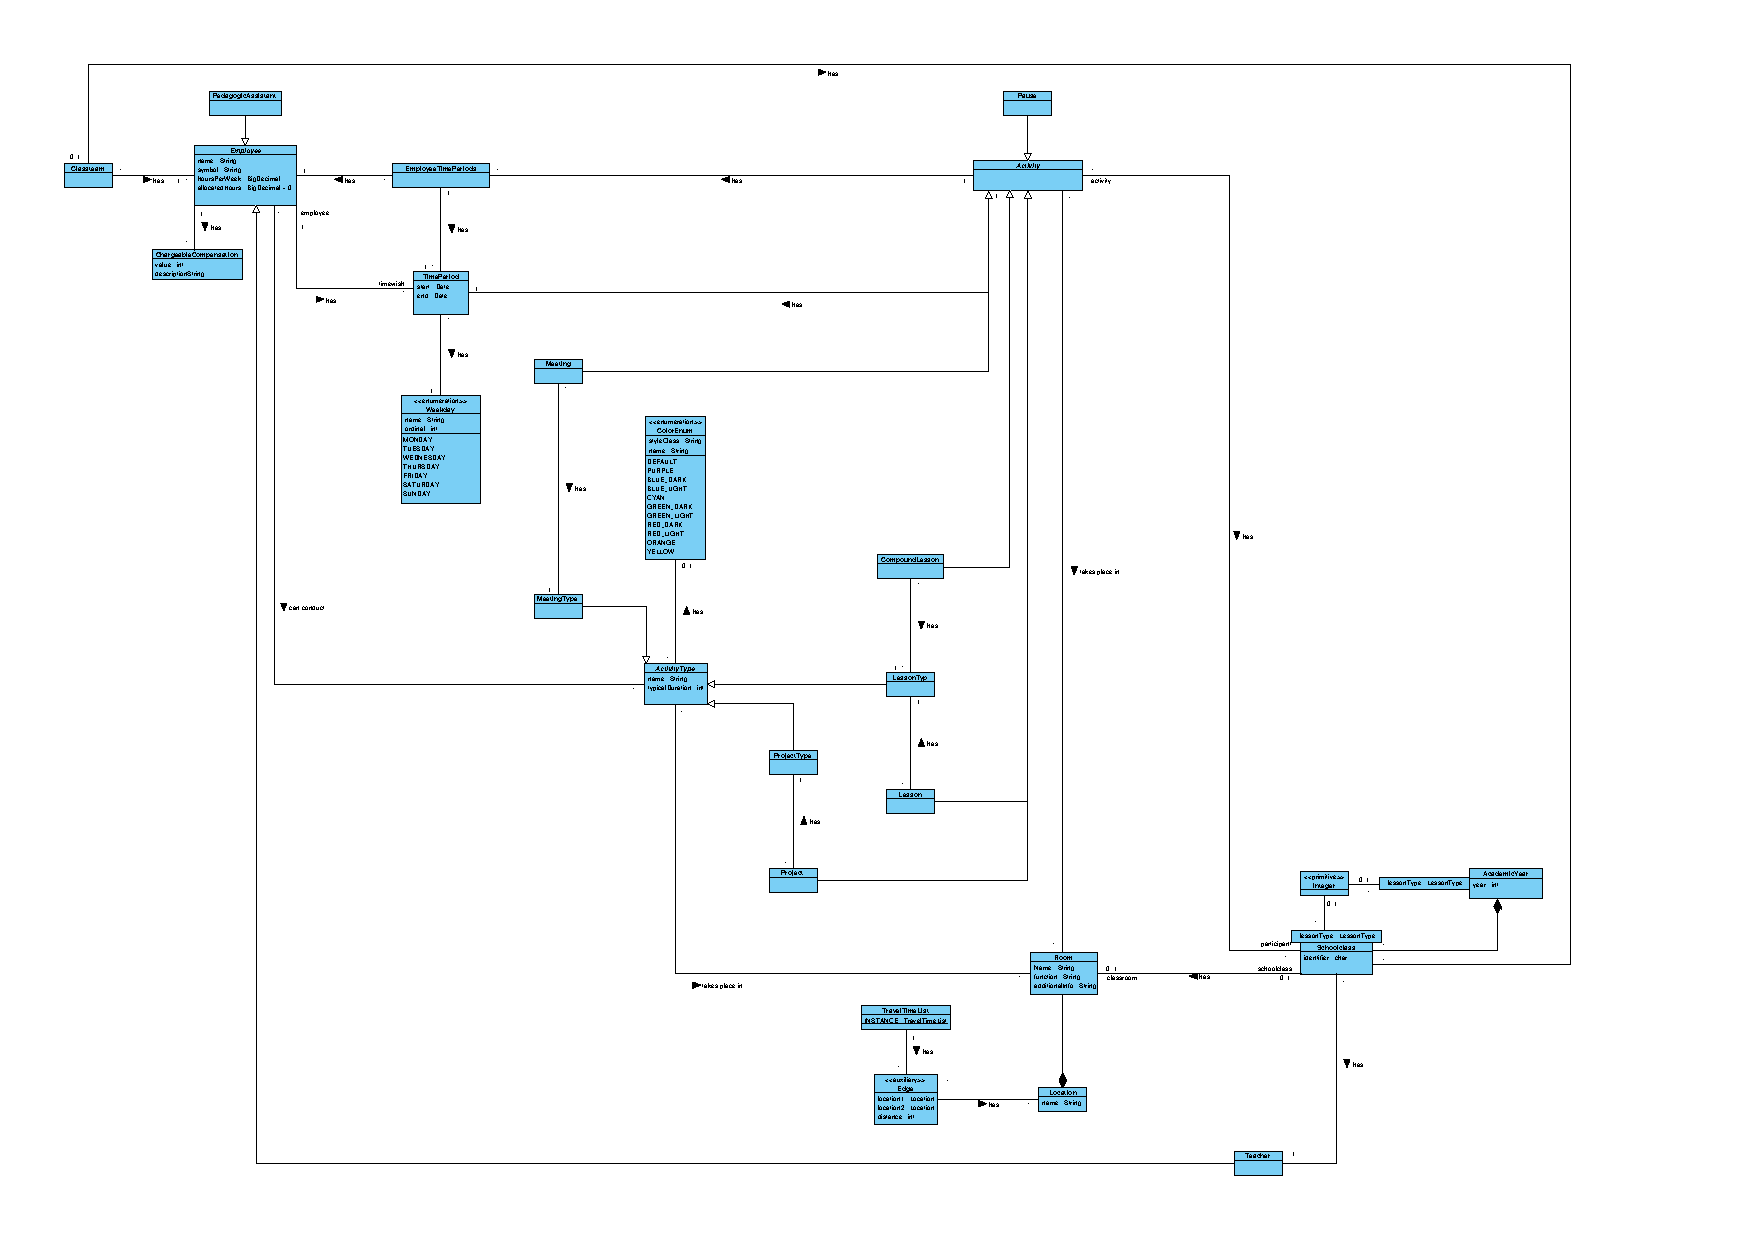
\includepdf[landscape]{datenmodell.pdf}
Im Folgenden soll die einzelnen Assoziationen erläutert werden.\\

\begin{tabularx}{\textwidth}{|p{0.6cm}|p{5cm}|X|}
\hline
\textbf{Nr.} & \textbf{Assoziation} & \textbf{Beschreibung} \\\hline
1 	& \textit{Employee} -- ChargeableCompensation	& Ein Mitarbeiter kann eine beliebige Anzahl
	an anrechenbaren Ersatzleistungen besitzen. Eine spezifische anrechenbare Ersatzleistung ist immer nur einem Mitarbeiter zugeordnet. \\\hline
2	& \textit{Employee} -- TimePeriod		& Ein Mitarbeiter hat eine beliebige Menge von 
	Zeiträumen als Zeitwünsche, also als Zeiten zu denen er gerne frei haben möchte. \\\hline
3	& \textit{Employee} -- \textit{ActivityType} & Einer beliebigen Anzahl von Mitarbeitern kann
	eine beliebige Anzahl von Aktivitätstypen als mögliche Stundeninhalte zugeordnet sein. Diese Assoziationen sind also komplett optional. \\\hline
4	& Schoolclass -- LessonType -- Integer \newline
	  AcademicYear -- LessonType -- Integer				& Eine Schulklasse und ein Jahrgang besitzen Unterrichtsbedarfe. Dies wird durch eine Zuordnung von Integer-Werten zu LessonType-Objekten realisiert. Jedes LessonType-Objekt darf in Kombination mit einer Klasse / einem Jahrgang nur einmal vorkommen. \\\hline
5	& Schoolclass -- Teacher 				& Eine beliebige Anzahl an Schulklassen hat genau
	einen Klassenlehrer. Ein Lehrer kann Klassenlehrer mehrerer Schulklassen sein. \\\hline
6	& AcademicYear -- Schoolclass 			& Ein AcademicYear-Objekt besteht aus einer beliebigen 
	Anzahl Schoolclass-Objekten. Wird das AcademicYear-Objekt gelöscht, werden auch alle dazu gehörigen Schoolclass-Objekte gelöscht.\\\hline
7	& \textit{Activity} -- TimePeriod				& Einer Aktivität steht immer genau ein
	Zeitraum gegenüber.\\\hline
8	& \textit{Activity} -- Room						& Eine Aktivität ist mindestens einen Raum, 
	kann aber auch mehreren Räumen zugeordnet sein.\\\hline
\end{tabularx}

\begin{tabularx}{\textwidth}{|p{0.6cm}|p{5cm}|X|}
\hline
9 	& \textit{Activity} -- EmployeeTimePeriods		& An einer Aktivität kann eine beliebige
	Anzahl an Mitarbeitern teilnehmen. Um realisieren zu können, dass diese früher gehen oder später kommen können, wird jedem Mitarbeiter eine eigene Liste von Zeiträumen zugeordnet. Dies wird durch die Klasse \texttt{EmployeeTimePeriods} umgesetzt. Einer Aktivität kann eine beliebige Zahl von EmployeeTimePeriods-Objekten zugeordnet sein, aber ein spezifisches EmployeeTimePeriod-Objekt ist immer nur genau einer Aktivität zugeordnet. \\\hline
10	& \textit{Activity} -- Schoolclass				& Eine beliebige Anzahl von Aktivitäten
	besitzt eine beliebige Anzahl von Schulklassen als Teilnehmer. Schulklassen können die Aktivität nicht
	frühzeitig verlassen, daher gilt für sie der für die Aktivität festgelegte Zeitraum.\\\hline
11	& Meeting -- MeetingType 			 & Eine Aktivität vom Typ Meeting hat genau einen
	MeetingType. Ein MeetingType kann mehreren Aktivitäten vom Typ Meeting zugeordnet sein. \\\hline
12	& Project -- ProjectType			& Eine Aktivität vom Typ Project hat genau einen
	ProjectType. Ein ProjectType kann mehreren Aktivitäten vom Typ Project zugeordnet sein. \\\hline
13	& Lesson -- LessonType				& Eine Aktivität vom Typ Lesson hat genau einen
	LessonType. Ein LessonType kann mehreren Aktivitäten vom Typ Lesson zugeordnet sein. \\\hline
14	& CompoundLesson -- LessonType & Eine CompoundLesson (Bandunterricht) hat mindestens eins bis 
	beliebig viele LessonType-Objekte. \\\hline
15 	& EmployeeTimePeriods -- Employee 				& Eine beliebige Anzahl
	EmployeeTimePeriods-Objekte besitzt genau einen Lehrer. Ein Lehrer kann Teil einer beliebigen Anzahl von EmployeeTimePeriods-Objekten sein. \\\hline
16	& EmployeeTimePeriods -- TimePeriod 			& Ein EmployeeTimePeriods-Objekt besitzt
	mindestens eine bis beliebig viele TimePeriod-Objekte. Ein spezifisches TimePeriod-Objekt ist immer nur Teil von genau einem EmployeeTimePeriods-Objekt. \\\hline
\end{tabularx}

\begin{tabularx}{\textwidth}{|p{0.6cm}|p{5cm}|X|}
\hline
17 	& TimePeriod -- Weekday & Ein TimePeriod-Objekt hat genau einen Wochentag, ein Wochentag kann 
	mehreren TimePeriod-Objekten zugeordnet sein.\\\hline 
18	& Location -- Room						& Ein Standort besteht aus beliebig vielen Räumen. 
	Wird der Standort gelöscht, werden auch die Räume gelöscht.\\\hline
19	& \textit{ActivityType} -- Room					& Einer beliebigen Anzahl von Aktivitätstypen
	kann die Ausführung in einer beliebigen Anzahl von Räumen zugeordnet sein. \\\hline
20	& \textit{ActivityType} -- ColorEnum 		& Ein Aktivitätstyp hat genau eine Farbe. Eine
	Farbe kann mehrere Aktivitätstypen zugeordnet sein.\\\hline
21	& Classteam -- Schoolclass 					& Ein Klassenteam hat eine beliebige Anzahl 
	Schulklassen, eine Schulklasse ist aber immer nur genau einem oder keinem Klassteam zugeordnet.\\\hline
22	& Classteam -- Employee 					& Ein Klassteam hat mindestens einen bis zu 
	einer beliebigen Anzahl Mitarbeiter. Wobei Klassenteams ohne mindestens eine Lehrkraft auf Logikebene verhindert werden müssen. Ein Mitarbeiter kann Teil mehrere Klassenteams sein. \\\hline
23	& TravelTimeList -- Edge 					& Ein TravelTimeList-Objekt kann eine beliebige
	Anzahl von Edge-Objekten besitzen. Ein Edge-Objekt kann nur Teil eines TravelTimeList-Objektes sein. \\\hline
24	& Edge -- Location							& Einer beliebigen Anzahl von Edge-Objekten stehen 
	immer genau zwei Location-Objekte gegenüber. Diese müssen disjunkt sein. \\\hline 
\end{tabularx}
\subsection{Datentypen und Repräsentation von Multiplizitäten}

Diese Abbildung stellt eine andere Sichtweise auf das vorher gezeigte Klassendiagramm von. Es wurden alle Assoziationen weggelassen und dafür die Attribute an die entsprechenden Klassen eingetragen.
\begin{figure}[H]
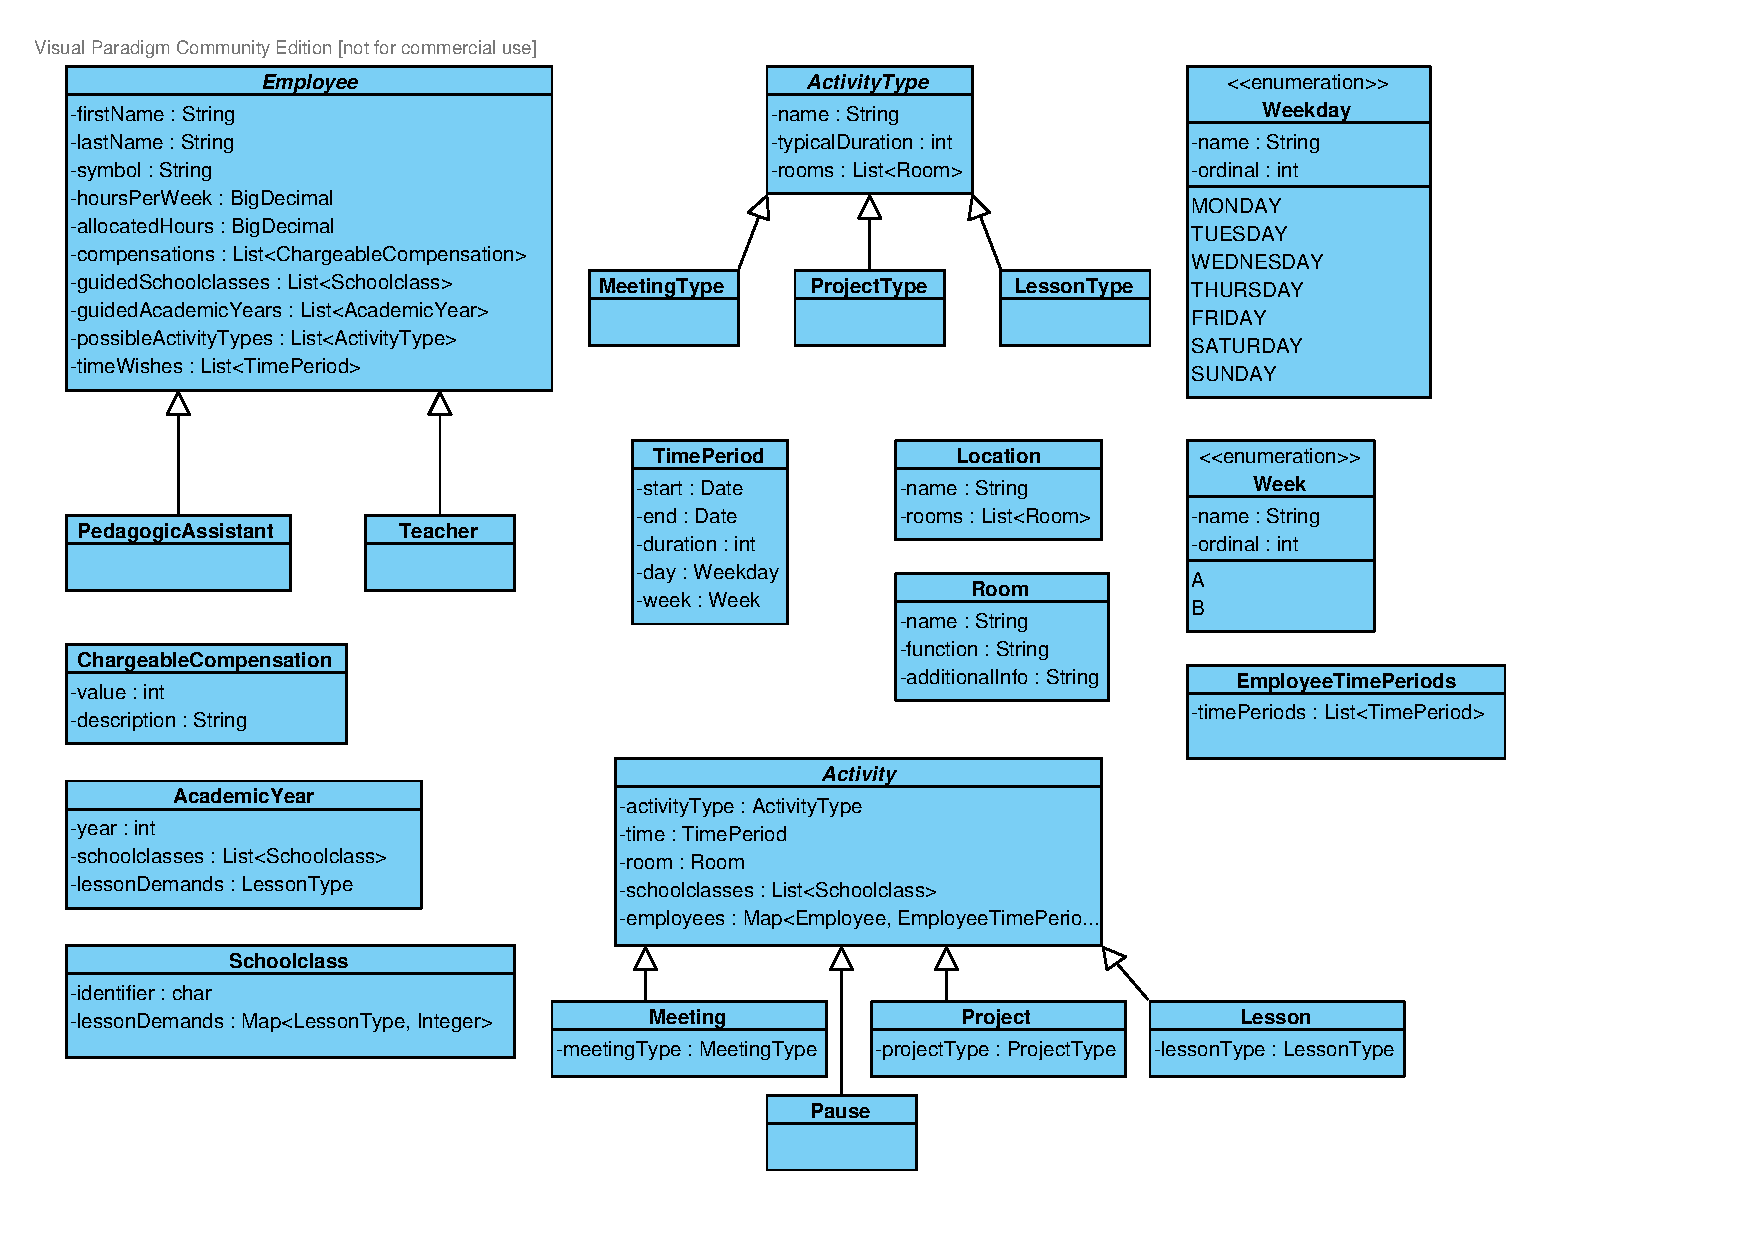
\includegraphics[width=\textwidth]{Datensicht.pdf}
\end{figure}


\subsection{Abbildung auf die Datenbank}
Die Abbildung auf die Datenbank erfolgt mithilfe des JPA-Frameworks Eclipselink. Damit muss lediglich darauf geachtet werden, die Attribute in den Klassen korrekt mit den One-To-Many- und Many-To-Many-Beziehungen gemäß des Datenmodells zu annotieren.\\

Folgende Klassen erhalten die \textit{Entity}-Annotation: 
\begin{itemize}
\item AcademicYear
\item Activity (und erbende Klassen)
\item ActivityType (und erbende Klassen)
\item Classteam
\item Employee (und erbende Klassen)
\item EmployeeTimePeriods
\item Location
\item Room
\item Schoolclass
\item TravelTimeList
\end{itemize}

Folgende Klassen erhalten die \textit{Embeddable}-Annotation:
\begin{itemize}
\item ChargeableCompensation
\item Edge
\item TimePeriod
\end{itemize}

\clearpage


\section{Ausführungssicht}
\label{sec:ausfuehrung}

\begin{figure}[H]
\centering
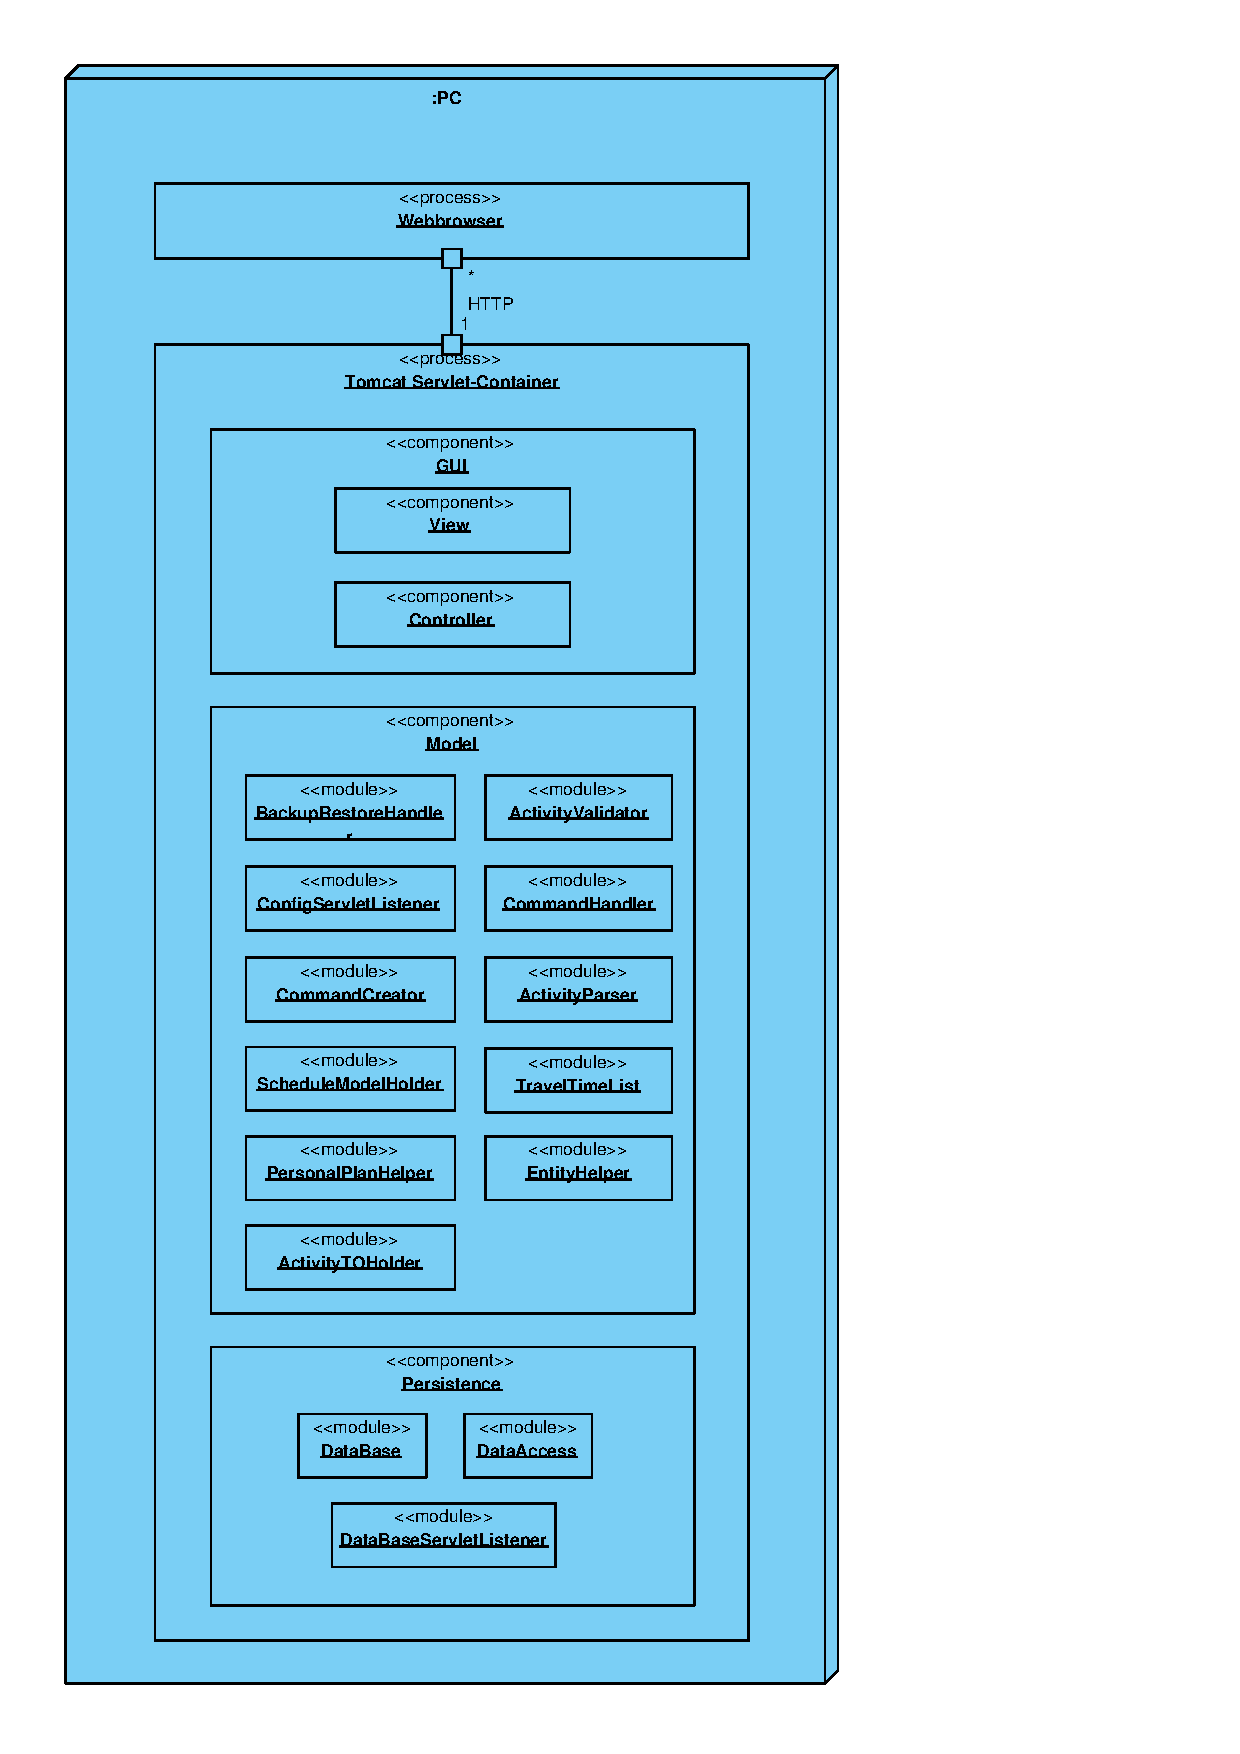
\includegraphics[width=0.5\textwidth]{ausfuehrung.pdf}
\end{figure}
Zur Laufzeit der Software wird auf dem ausführenden Rechner mindestens der Tomcat Servlet-Container als Prozess ausgeführt. Wenn die Software nicht nur im Hintergrund läuft, sondern auch damit gearbeitet wird, läuft außerdem ein Webbrowser auf dem ausführenden Rechner. Der Webbrowser-Prozess kommuniziert via HTTP-Anfragen mit dem Tomcat Servlet-Container.\\
Die gesamte Geschäftslogik läuft innerhalb des Tomcat Servlet-Containers ab. \\
Im oben dargestellten Diagramm sind neben den \texttt{ServletContextListener} implementierenden Klassen (\texttt{BackupRestoreHandler}, \texttt{ConfigServletListener}, \texttt{DataBaseServletListener}) als Module alle Singleton-Klassen der Software aufgeführt, da von diesen zur Ausführung immer genau eine Instanz existiert. \\
Aus der Controller-Komponente sind während der Ausführung jeweils nur die Controller instanziiert, welche als Backing Beans für die gerade dargestellte JSF-Seite benötigt werden. Auch die Datenobjekte sind innerhalb der Software nur instanziiert, sofern sie gerade angezeigt werden. Ansonsten können sie sich ggf. im Datenbank-Cache befinden.

\section[Zusammenhänge zwischen Anwendungsfällen und Architektur]{Zusammenhänge zwischen Anwendungsfällen und Architektur\sectionmark{Zusammenhänge AF u. Architektur}}
\sectionmark{Zusammenhänge AF u. Architektur}
\label{sec:anwendungsfaelle}

\subsection{Erfolgreiches Hinzufügen einer Aktivität (Unterrichtsstunde)}
\label{subsec:addActivitySuccess}
Das auf den folgenden Seiten dargestellte Sequenzdiagramm zeigt den Ablauf des erfolgreichen Hinzufügens eines Lesson-Objektes. Das Diagramm wurde der Übersichtlichkeit halber auf mehrere Seiten verteilt. Über die jeweiligen Lebenslinien wurde noch einmal geschrieben, welches Objekt zu dieser gehört. Im dritten und vierten Teil des Diagramms wurden alle für die aufgeführten Schritte irrelevanten Lebenslinien entfernt, um das Diagramm weiterhin in einer lesbaren Größe vorliegen zu haben. \\

Das erste Diagramm zeigt den Schritt der Validierung der Parameterwerte der hinzuzufügenden Aktivität. Nach Aufruf von \textit{addLesson} wird zunächst die Methode \textit{validateActivity(Activity, TimePeriod)} auf dem \texttt{ActivityValidator} aufgerufen. Diese Methode prüft dann durch Aufrufe von anderen im \texttt{ActivityValidator} enthaltenen Methoden, ob die Aktivität den Stundenplänen von allen gewählten Teilnehmern hinzugefügt werden kann oder ob es dabei zu Überschneidungen kommt. Da es sich hier um das erfolgreiche Hinzufügen handelt, wird von jeder der Validierungsmethoden ein \texttt{SuccessStatus} erhalten. \\

Im zweiten Diagramm ist dann dargestellt, wie das zum Hinzufügen der Aktivität benötigte Command erzeugt wird. Es wird die Methode \textit{createEmployeeUpdateAddWorkingHours(Activity)} der Klasse \texttt{CommandCreator} aufgerufen. Diese erzeugt ein \texttt{MacroCommand}, welches allen an der Aktivität teilnehmenden Mitarbeitern die Dauer ihrer Teilnahme zu den verteilten Stunden hinzufügt, also deren Auslastung erhöht. Der Prozess der Macro-Erstellung ist im Diagramm auch aufgeführt. Dabei wird je nachdem, ob es sich um einen Lehrer oder einen päd. Mitarbeiter handelt, die Dauer der Teilnahme dieser Person (summierte Dauer aller \texttt{TimePeriod}-Objekte des zugehörigen \texttt{EmployeeTimePeriods}) durch die Zahl dividiert, welche die zeitliche Abrechnung der Person angibt. Dies ergibt die Dauer der Teilnahme an der Aktivität in einer gemäß dem vorhandenen Wert gültigen Einheit. Es wird ein \texttt{Memento} des \texttt{Employee}-Objektes erzeugt. Anschließend wird der vorher berechnete Wert zu den verteilten Stunden des \texttt{Employee} hinzugefügt. Schließlich wird ein \texttt{UpdateCommand} für den \texttt{Employee} erstellt und dem \texttt{MacroCommand} hinzugefügt. Das erzeugte \texttt{MacroCommand} wird dann an den \texttt{LessonController} zurückgegeben (1.2.14). Dieser ruft auf dem \texttt{MacroCommand} noch die Methode \textit{add(ICommand)} auf und fügt ihm ein neues \texttt{AddCommand} für die Aktivität hinzu. \\

Anschließend wird die Methode \textit{execute(ICommand)} auf dem \texttt{CommandHandler} mit dem vorher erzeugten \texttt{MacroCommand} als Parameter aufgerufen. Der \texttt{CommandHandler} ruft auf dem Command die \textit{execute}-Methode auf. Da der \texttt{CommandHandler} nicht weiß, was für ein konkretes Command er ausführt, ist der weitere Ablauf im Diagramm nicht dargestellt. In diesem Fall würde der \texttt{CommandHandler} ein \texttt{MacroCommand} ausführen, welches aus einer beliebigen Zahl \texttt{UpdateCommands} und zuletzt einem \texttt{AddCommand} bestehen würde. Die Ausführung dieser Commands würde dann jeweils die Methode \textit{update(Entity)} bzw. \textit{add(Entity)} der Klasse \texttt{DataAccess} aufrufen. Von dem \textit{execute}-Aufruf wird ein \texttt{SuccessStatus} zurückgegeben. Das Command wird der Undo-Liste hinzugefügt und die Redo-Liste wird komplett geleert. Das vom Aufruf der \textit{execute}-Methode auf dem Command erhaltene \texttt{SuccessStatus}-Objekt wird an den \texttt{LessonController} zurückgegeben (1.6.5). \\

Daraufhin ruft der LessonController seine \textit{init}-Methode auf, damit für das nächste Hinzufügen einer Unterrichtsstunde, auf einem neuen \texttt{Lesson}-Objekt gearbeitet wird. Außerdem wird die aktuelle Instanz des \texttt{RequestContext} geholt und darauf die \textit{execute}-Methode mit dem Skript zum Schließen des Dialogs aufgerufen.
Anschließend wird auf dem \texttt{ScheduleModelHolder} die Methode \textit{updateScheduleModel} aufgerufen, um den Stundenplan zu aktualisieren. Auf dem vorher erhaltenen \textit{SuccessStatus}-Objekt wird dann die Methode \textit{report} aufgerufen, welche eine \texttt{FacesMessage} zurückgibt. Diese wird dem \texttt{FacesContext} hinzugefügt. \\
Damit ist das Hinzufügen des \texttt{Lesson}-Objektes abgeschlossen.

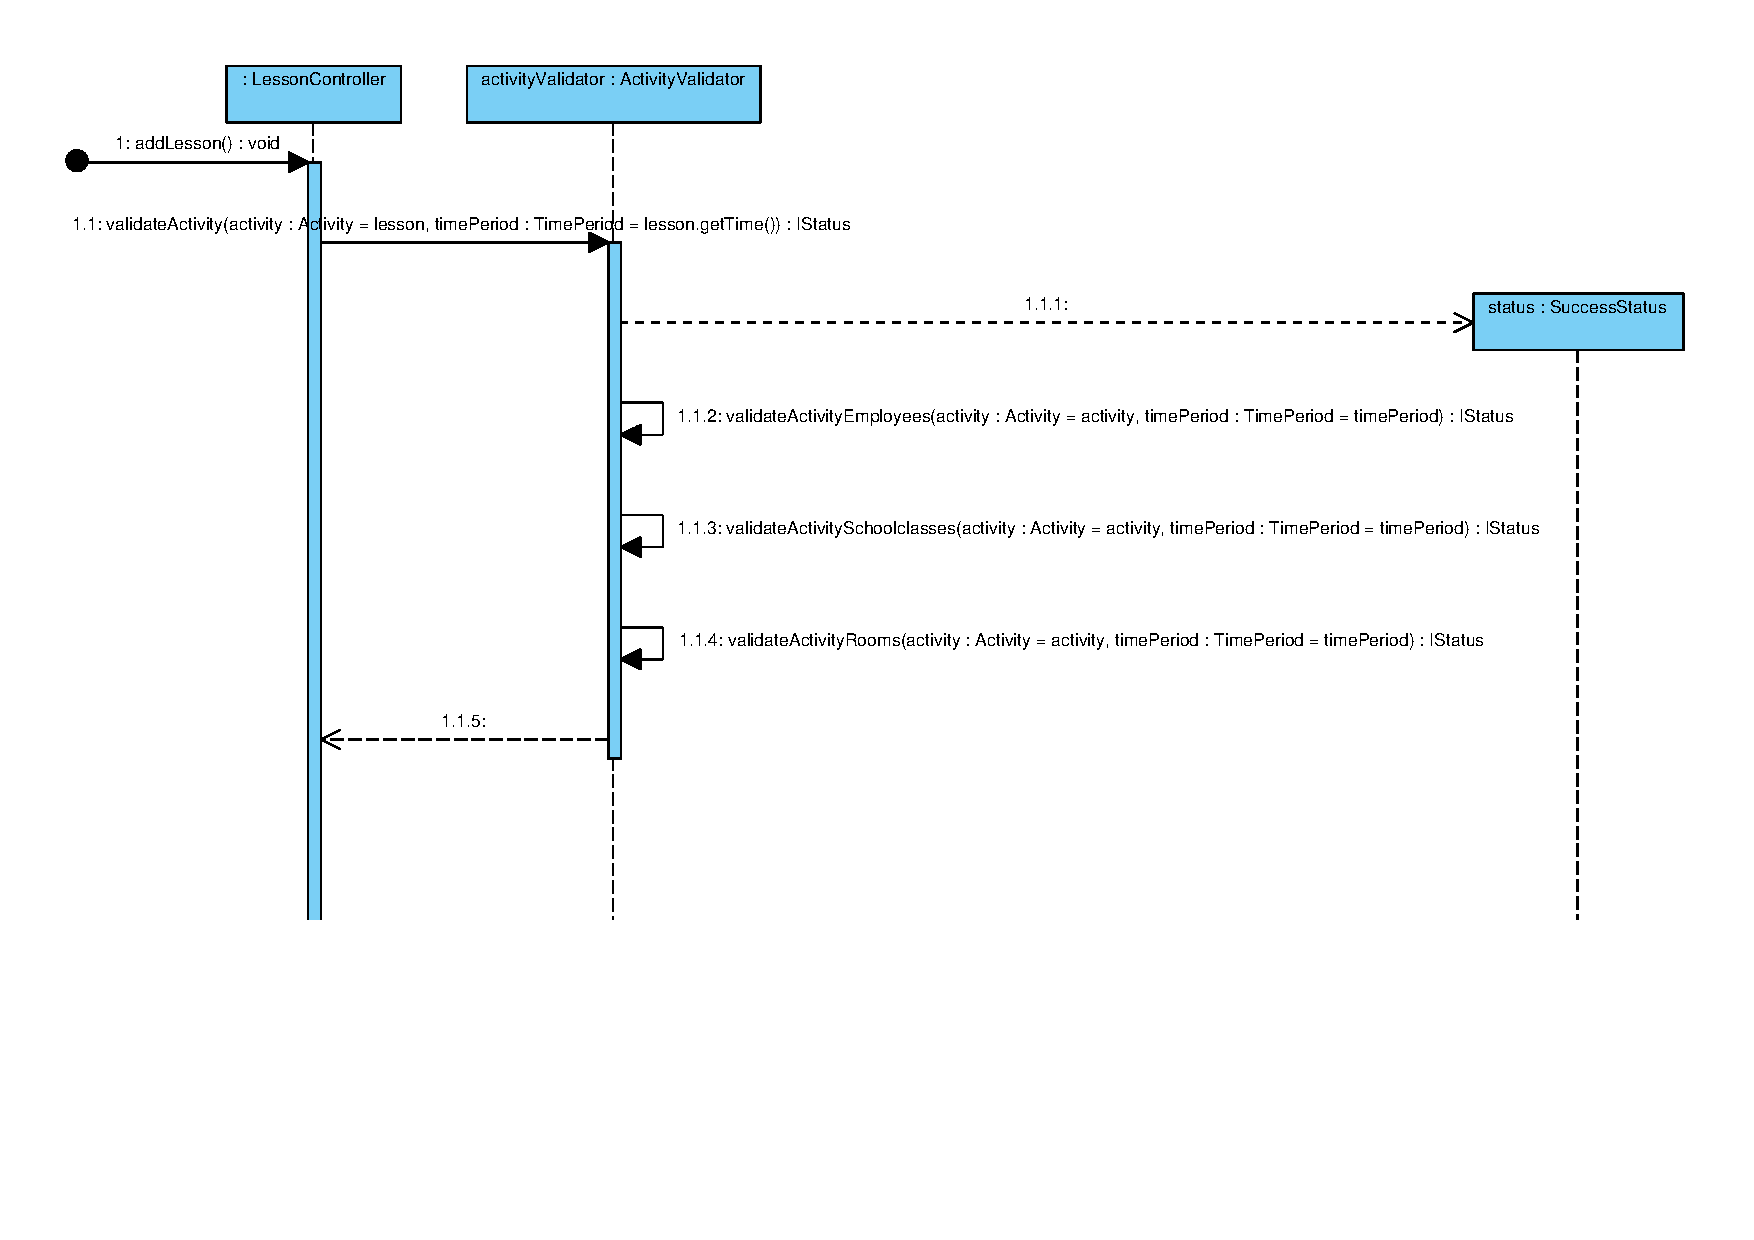
\includepdf[landscape]{addLessonSequence1.pdf}

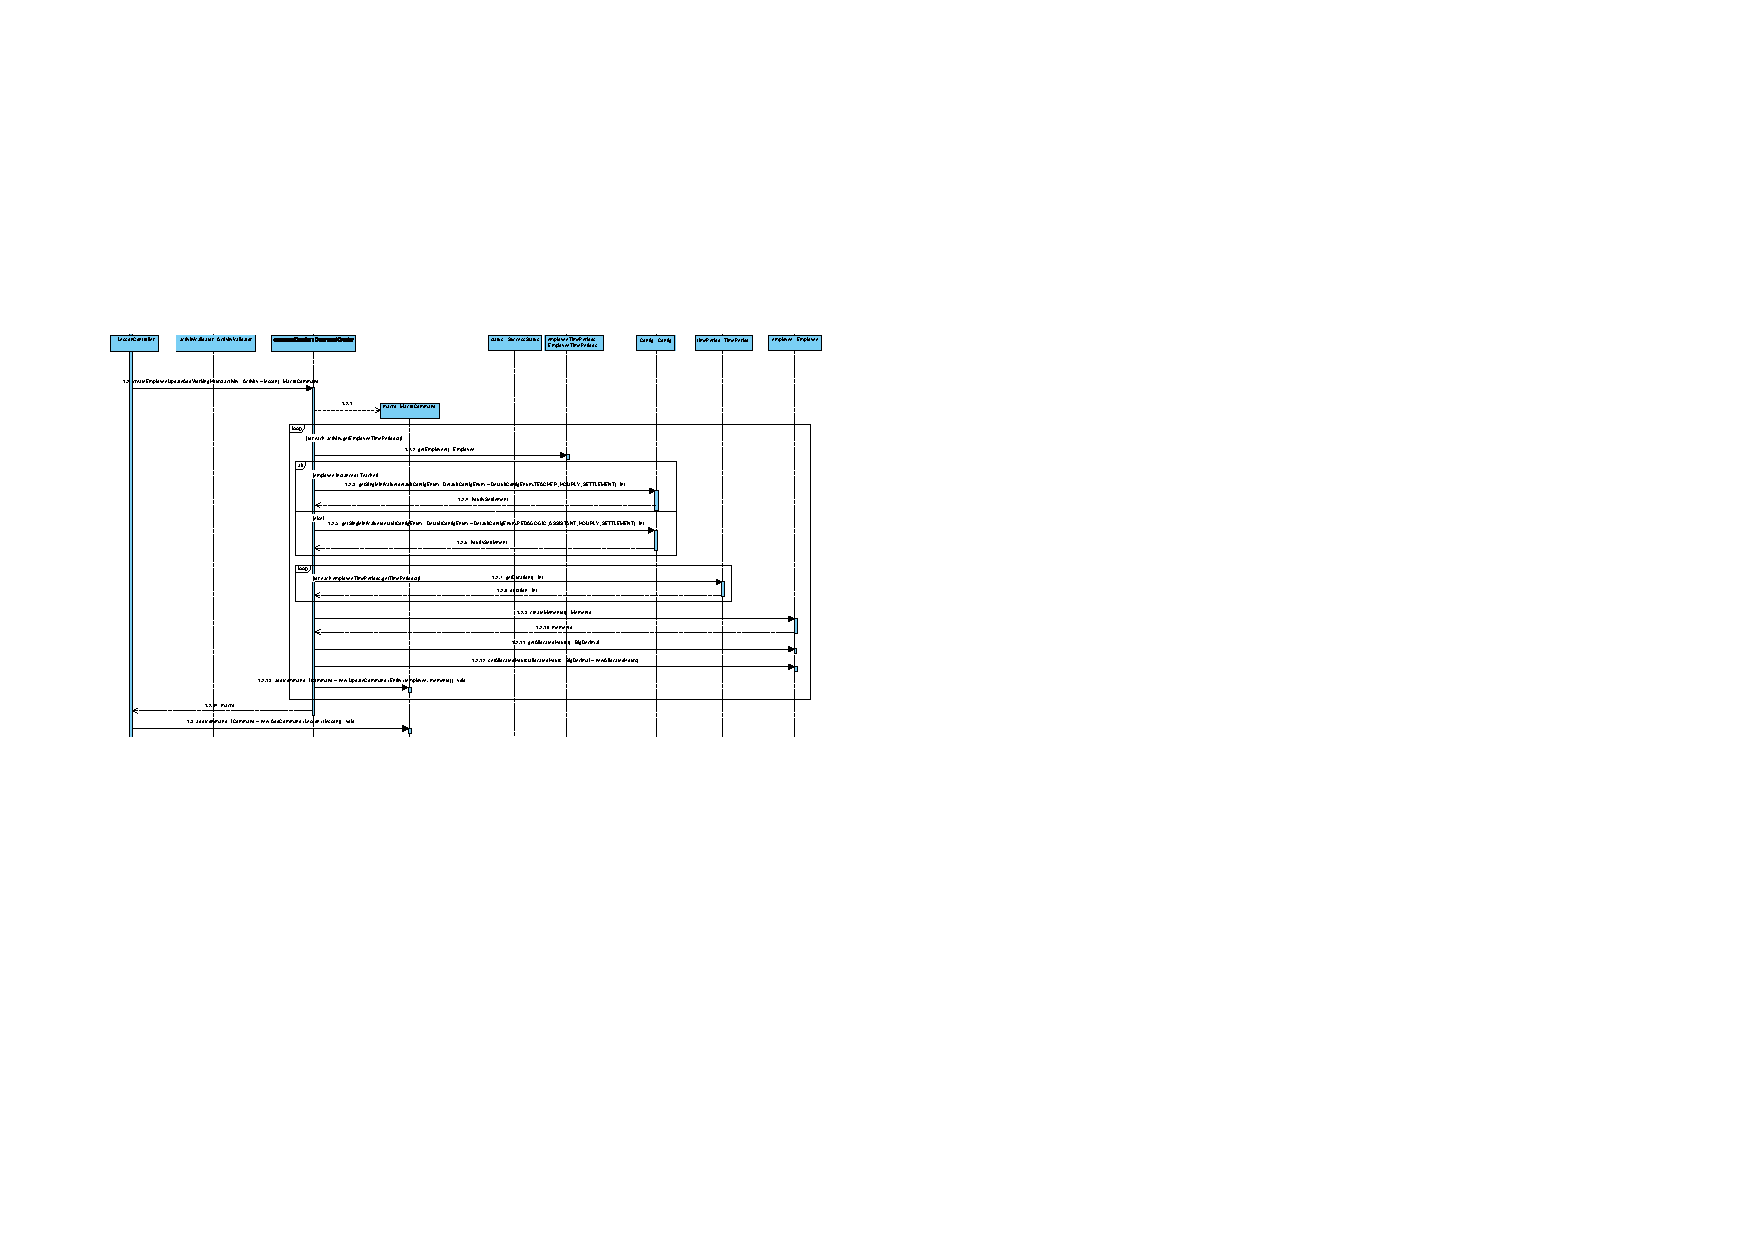
\includepdf[landscape]{addLessonSequence2.pdf}

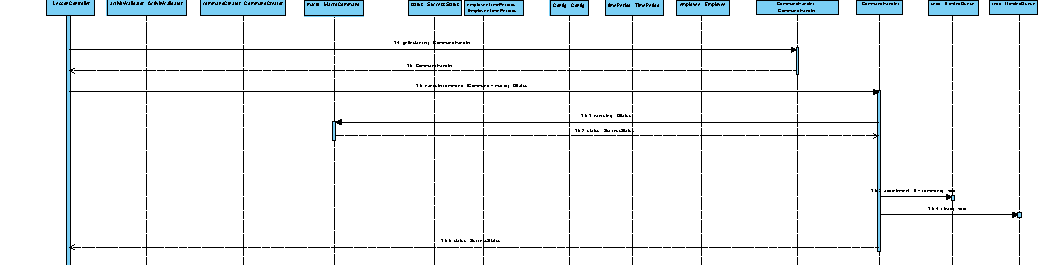
\includepdf[landscape]{addLessonSequence3.pdf}

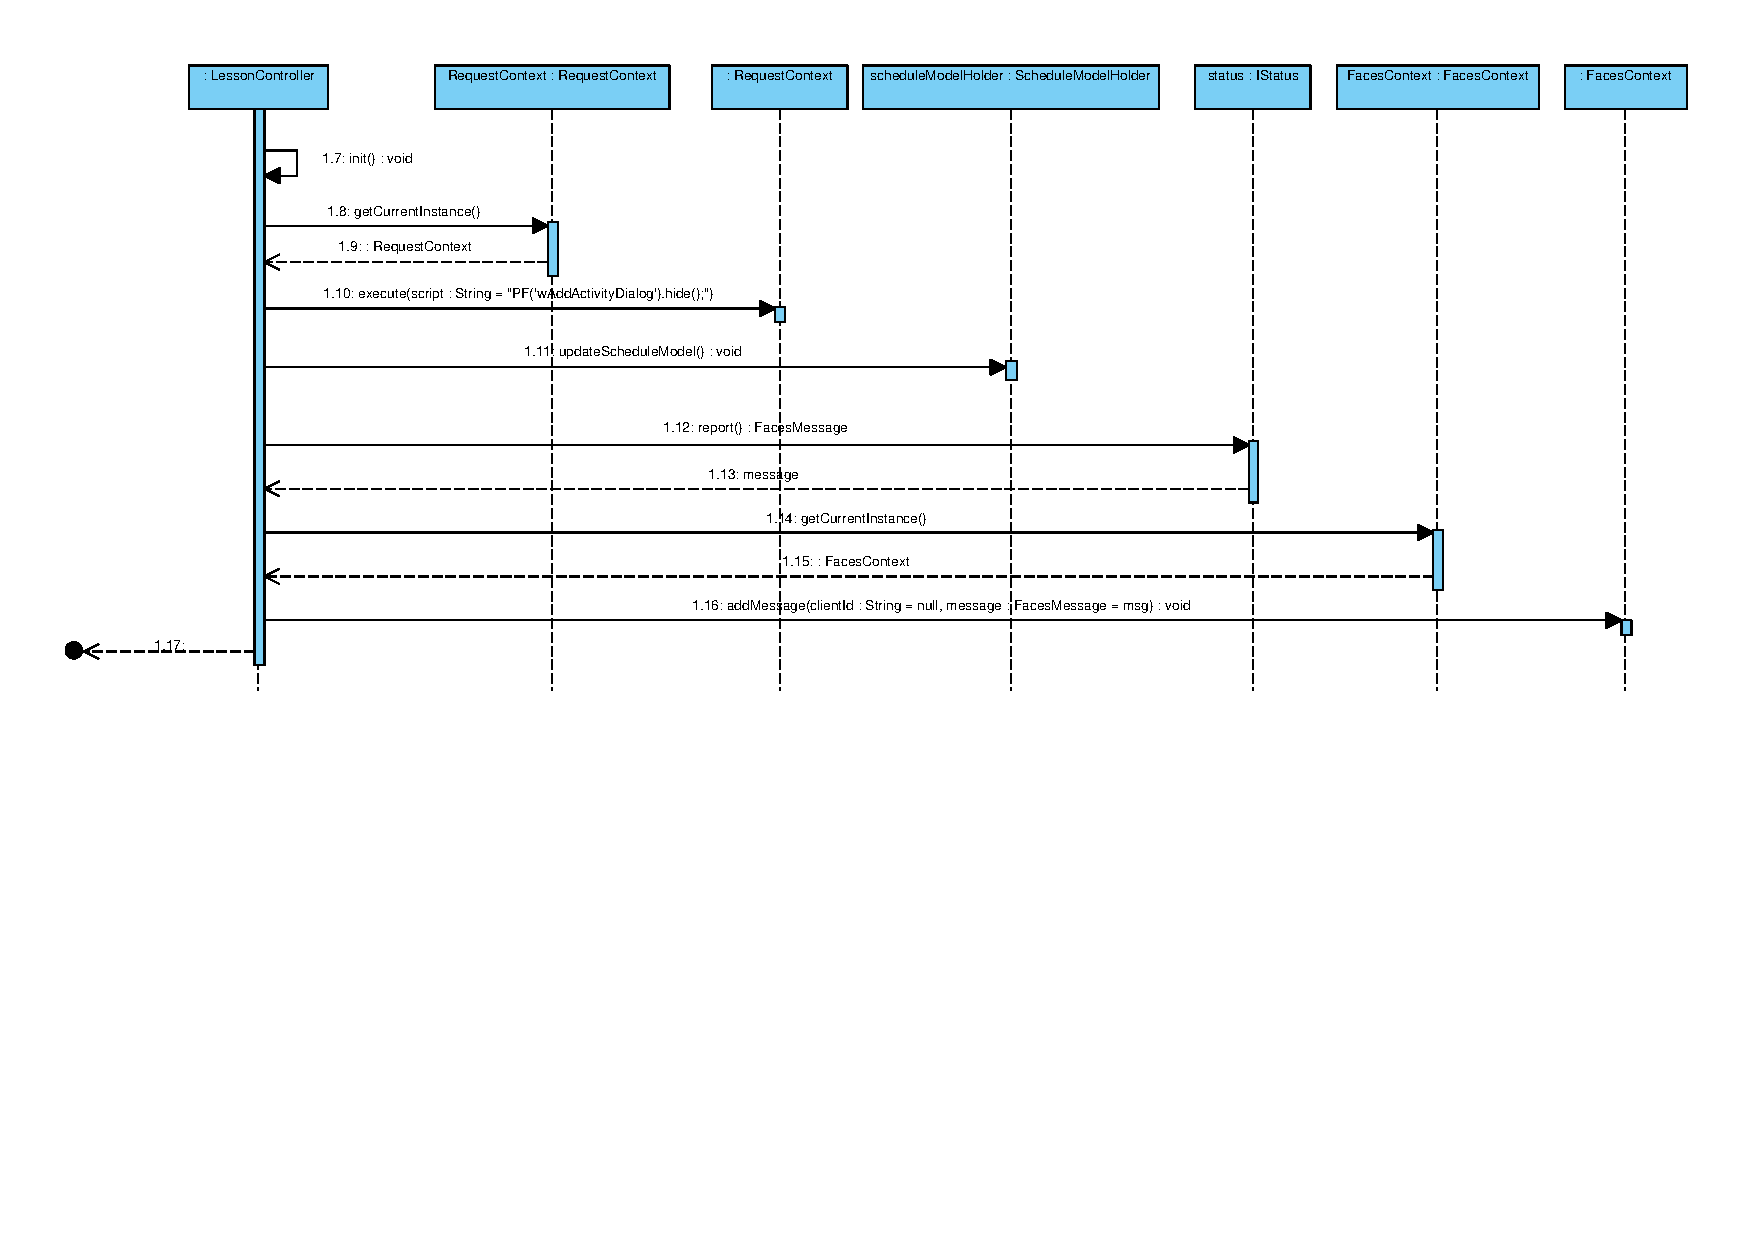
\includepdf[landscape]{addLessonSequence4.pdf}

\subsection{Fehlgeschlagenes Hinzufügen einer Aktivität (Unterrichtsstunde)}
Das auf der folgenden Seite dargestellte Diagramme zeigt den Ablauf des im vorherigen Kapitel \ref{subsec:addActivitySuccess} erläuterten Anwendungsfalls, wenn die Validierung zu Beginn fehlschlägt. Dazu muss von einer der von \textit{validateActivity(Activity, TimePeriod)} aufgerufenen Methoden ein \texttt{FailureStatus} zurückgegeben werden, denn dann gibt auch die Methode \textit{validateActivity(Activity, TimePeriod)} einen \texttt{FailureStatus} zurück. Hier ist nicht näher angegeben, welche der Methoden einen \texttt{FailureStatus} zurückgibt, das vorgehen bleibt aber ohnehin dasselbe. \\
Wird also von \textit{validateActivity(Activity, TimePeriod)} ein \texttt{FailureStatus} zurückgegeben, wird auf diesem \texttt{IStatus}-Objekt die Methode \textit{report} aufgerufen, um die enthaltene \texttt{FacesMessage} zu erhalten. Anschließend wird die aktuelle Instanz des \texttt{FacesContext} geholt und die Nachricht hinzugefügt, so dass der Nutzer über den Fehlschlag informiert werden kann. Damit ist der Anwendungsfall abgeschlossen.


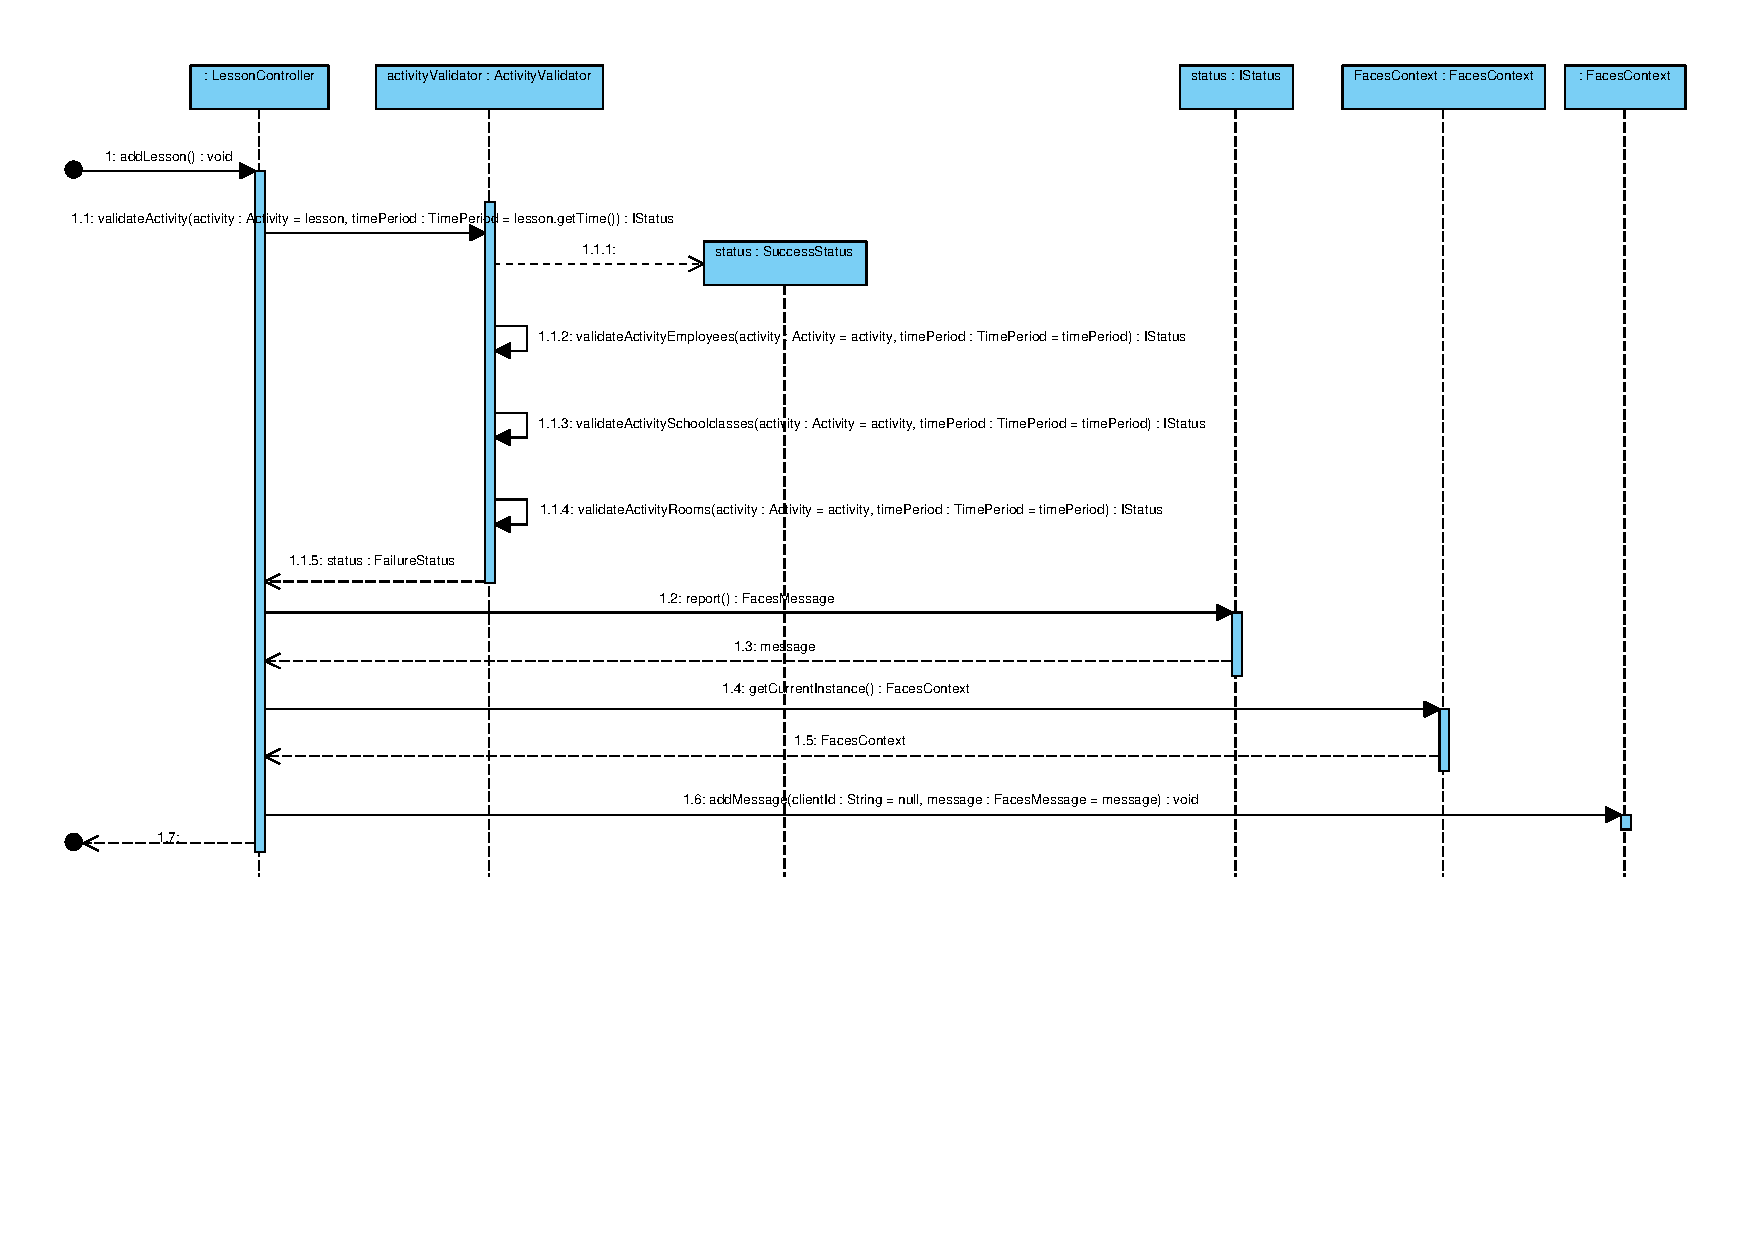
\includepdf[landscape]{addLessonFailSequence.pdf}

\subsection{Erfolgreiches Hinzufügen einer Lehrkraft}
Das Sequenzdiagramm auf der nächsten Seite stellt den Ablauf des erfolgreichen Hinzufügens einer Lehrkraft dar.\\
Nach dem Aufruf von \textit{addTeacher} auf dem \texttt{TeacherController} wird zunächst ein neues \texttt{AddCommand} erstellt. Dieses wird als Parameter an die Methode \textit{execute(ICommand)} des \texttt{CommandHandler} übergeben. Der \texttt{CommandHandler} ruft dann die \textit{execute}-Methode auf dem Command auf. Diese ruft auf dem  enthaltenen \texttt{Entity}-Objekt die \textit{persist}-Methode auf, welche die \textit{persist(Entity)}- Methode der Klasse \texttt{DataAccess} mit dem \texttt{Entity}-Objekt selbst als Parameter aufruft. Dadurch wird dieses Objekt in der Datenbank gespeichert. Anschließend wird ein neues \texttt{SuccessStatus}-Objekt erstellt und an den \texttt{CommandHandler} zurückgegeben.\\
Der \texttt{CommandHandler} fügt dann das ausgeführte \texttt{AddCommand} der Undo-Liste hinzu und leert die Redo-Liste. Anschließend wird das \texttt{SuccessStatus}-Objekt an den \texttt{TeacherController} zurückgegeben.\\
Dort wird auf dem \texttt{SuccessStatus}-Objekt zunächst die \textit{report}-Methode aufgerufen, welche eine \texttt{FacesMessage} zurückgibt, die über den Erfolg bzw. Misserfolg informiert. Außerdem wird ein neues leeres \texttt{Teacher}-Objekt erzeugt, damit beim nächsten Hinzufügen einer Lehrkraft auf einem anderen \texttt{Teacher}-Objekt gearbeitet wird.\\
Schließlich wird die vorher erhaltene \texttt{FacesMessage} dem \texttt{FacesContext} hinzugefügt. Damit ist das Hinzufügen der Lehrkraft abgeschlossen.


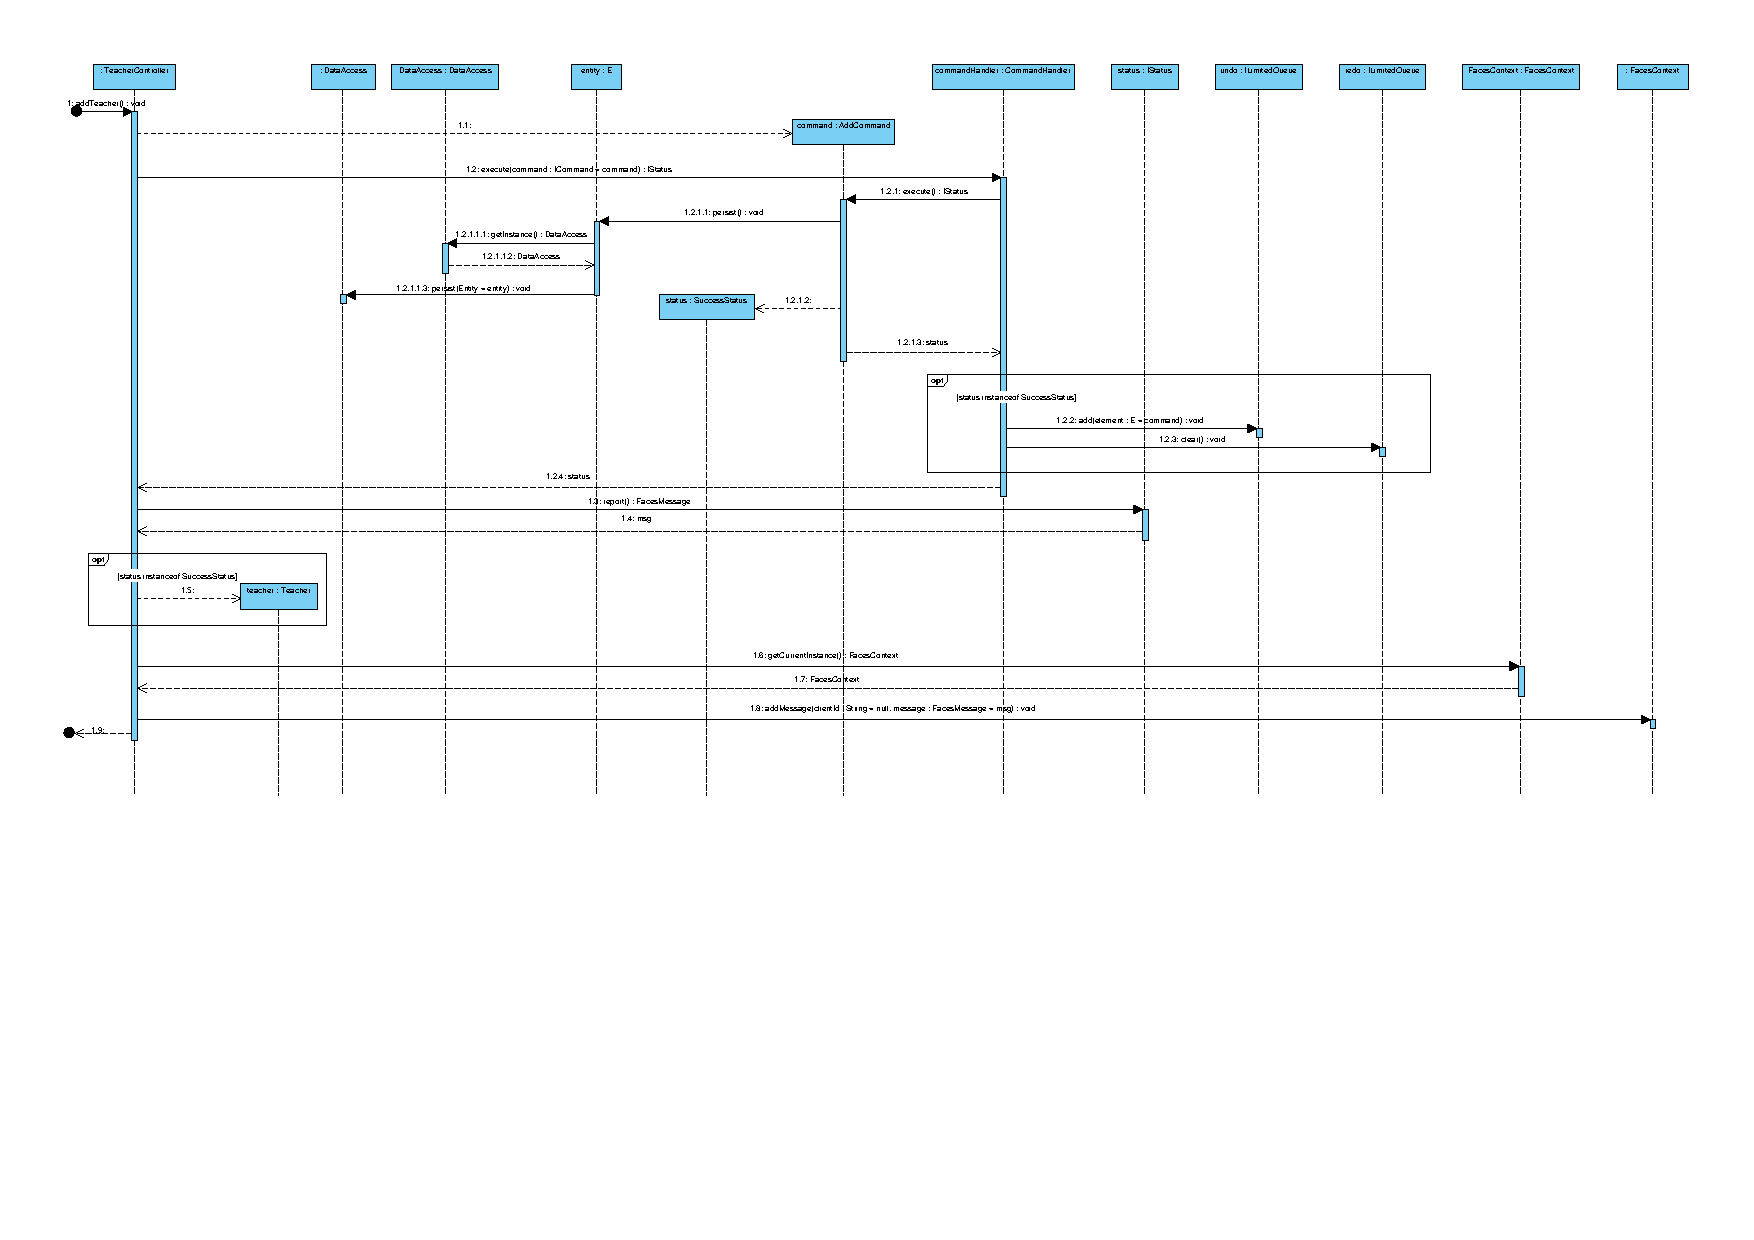
\includepdf[landscape]{addTeacherSequence.pdf}

\section{Evolution}
\nurlangversion

\label{sec:evolution}

{\it
  Beschreibt in diesem Abschnitt, welche Änderungen Ihr
  vornehmen müsst, wenn sich Anforderungen oder Rahmenbedingungen
  ändern. Insbesondere sollten hierbei die in der
  Anforderungsspezifikation unter "`Ausblick"' bereits genannten
  Punkte behandelt werden.}

\dots


\end{document} 
